\documentclass[hyper,dissertation]{MUthesis}
%% options:
%%  doublespace  -- the default, indicates double spacing as per MU
%%                  requirements; use for all final copies
%%  singlespace  -- for early work; not acceptable for final draft
%%  dissertation -- default; indicates this is a dissertation
%%  thesis       -- indicates this is a Master's thesis; changes the default
%%                  for \degree{}{} to Master of Science / M.S.
%%  nolisthyphen -- disallows hyphenation in the Table of Contents and
%%                      the list of figures/tables; only use if the graduate
%%                      school or your committee complain
%%  nohyphen     -- disallows hyphenation /everywhere/; don't use unless
%%                  someone complains (and even then, fight back!)
%%  hyperpages   -- default; loads hyperref with stripped down options
%%  hyper        -- loads hyperref with page labels and invisible links
%%  nohyper      -- turns off loading of hyperref, which is used only to
%%                  fix page labels (so that i is called i, not 1, in the PDF);
%%                  use this if you want to load hyperref with other options
%%
%%  All other options are passed as-is to the "report" class; the default size
%%  is 12pt, but you can specify 10 or 11 pt (or any other size supported by
%%  "report")

\usepackage{amsmath}
\usepackage{amssymb}
\usepackage{physics}
%\usepackage{txfonts}
%\usepackage{pxfonts}
\usepackage{newpxtext, newpxmath}
%\usepackage[largesc,osf]{newpxtext, newpxmath}
\usepackage{graphicx}
%\usepackage{achemso}
\usepackage{textgreek}
\usepackage{miller}
\usepackage{comment}
\usepackage{siunitx}
\usepackage[version=4]{mhchem}
\usepackage{rotating}


\usepackage[rootbib]{chapterbib}
%\usepackage{chapterbib}
%\begin{comment}
\usepackage{booktabs}
\usepackage[overload]{textcase}
\usepackage{xcolor}
%\usepackage{cite}
\usepackage{setspace}
\usepackage{nomencl}
\usepackage{tikz}
\usepackage{listings}
\usepackage[numbers,square,sort&compress]{natbib}
\usepackage[toc,page]{appendix}
%\usepackage[titletoc]{appendix}
%\addtolength{\nomlabel}{0.8cm}


\usetikzlibrary{shapes.geometric, arrows}

\tikzstyle{block2} = [rectangle, draw,
     text centered,  rounded corners=5pt, line width=0.4mm, minimum height=3em]
\tikzstyle{alp's} = [ellipse, draw,
	text width=2em, text centered]

\tikzstyle{block3} = [rectangle, draw,
	text width=20em, text centered, minimum height=3em, rounded corners=10pt]

\tikzstyle{decision} = [diamond, draw,
	 text centered, aspect=2.5, line width=0.4mm]



\tikzstyle{line} = [thick, ->, >=stealth, draw, line width=0.51mm, -latex']
\tikzstyle{cloud} = [draw, ellipse,fill=red!20, node distance=3cm,
    minimum height=2em]

\tikzstyle[arrow] = [thick, ->, >=stealth]

\definecolor{categorize}{rgb}{0,0.6,0}
\definecolor{codegray}{rgb}{0.5,0.5,0.5}
\definecolor{codepurple}{rgb}{0.58,0,0.82}
\definecolor{backcolour}{rgb}{0.95,0.95,0.92}

\lstdefinestyle{deflt}{
commentstyle=\color{codegray},
	keywordstyle=\color{black},
	numberstyle=\tiny\color{codegray},
	stringstyle=\color{black},
	basicstyle=\linespread{0.9}\ttfamily\footnotesize,
	breakatwhitespace=false,         
	breaklines=true,                 
	captionpos=b,                    
	keepspaces=true,                 
	numbers=left,                    
	numbersep=5pt,                  
	showspaces=false,                
	showstringspaces=false,
	showtabs=false,                  
	tabsize=2,
	xleftmargin=2.0ex,
}

\lstdefinestyle{cpp}{
	commentstyle=\color{codegray},
	keywordstyle=\color{black},
	numberstyle=\tiny\color{codegray},
	stringstyle=\color{black},
	basicstyle=\linespread{0.9}\ttfamily\footnotesize,
	breakatwhitespace=false,         
	breaklines=true, 
	%morecomment=[1]{//},
	morecomment=[s]{/*}{*/},
	morecomment=[l]{//},
	captionpos=b,                    
	keepspaces=true,                 
	numbers=left,                    
	numbersep=5pt,                  
	showspaces=false,                
	showstringspaces=false,
	showtabs=false,                  
	tabsize=2,
	xleftmargin=2.0ex,
}
\lstdefinestyle{atpw}{
	commentstyle=\color{codegray},
	keywordstyle=\color{black},
	numberstyle=\tiny\color{codegray},
	stringstyle=\color{black},
	basicstyle=\linespread{0.9}\ttfamily\footnotesize,
	breakatwhitespace=false,         
	breaklines=true, 
	%morecomment=[s]{/*}{*/},
	morecomment=[l]{!},
	captionpos=b,                    
	keepspaces=true,                 
	numbers=left,                    
	numbersep=5pt,                  
	showspaces=false,                
	showstringspaces=false,
	showtabs=false,                  
	tabsize=2,
	xleftmargin=2.0ex,
}

\lstdefinestyle{pythn}{
	commentstyle=\color{codegray},
	keywordstyle=\color{black},
	numberstyle=\tiny\color{codegray},
	stringstyle=\color{black},
	basicstyle=\linespread{0.9}\ttfamily\footnotesize,
	breakatwhitespace=false,         
	breaklines=true, 
	%morecomment=[s]{/*}{*/},
	morecomment=[l]{\#},
	captionpos=b,                    
	keepspaces=true,                 
	numbers=left,                    
	numbersep=5pt,                  
	showspaces=false,                
	showstringspaces=false,
	showtabs=ture,
	tabsize=2,
	xleftmargin=2.0ex,
}

\DeclareRobustCommand{\schrod}{Schr\"odinger }

\graphicspath{{images/}}
%\makenomenclature
%\makeglossary
\newcommand*{\ie}{\emph{i.e.}}
\newcommand*{\eg}{\emph{e.g.}}
\makeatletter
\DeclareRobustCommand{\etal}{\emph{et al}\@ifnextchar.{}{.}}
\makeatother
\makenomenclature
\DeclareGraphicsExtensions{.pdf,.png,.jpg,.mps}

%\title{The Impact of Fission gas on Uranium--Molybdenum Fuel}
\title{Influence of Inert Gases on Heat and Mass Transfer in Next-Generation Nuclear Reactors}
\author{Abu Rafi Mohammad Iasir}
\date{May 2021}
\copyrightyear{2021}
                
\chair{Karl Hammond}
\firstreader{Scott Kovaleski}
\secondreader{Robert Winholtz}
\thirdreader{Nickie Peters}

%% Your degree's name;
%\degree{Doctor of Philosophy}{Ph.D.}
%% defaults to {Doctor of Philosophy}{Ph.D.} (option "dissertation"; default)
%% defaults to {Master of Science}{M.S.} for theses (option "thesis")

\begin{document}
\frontmatter   % optional (automatically set at \begin{document})
\maketitle     % mandatory
\copyrightpage % optional
\approvalpage  % mandatory

\begin{dedication}
To my parents Ismail and Halima 
\end{dedication}

\begin{epigraph}{\textit{Rumi}}
``\textit{Do you think that I know what I am doing? \\
  That for one breath or half-breath I belong to myself?\\
  As much as a pen knows what it's writing,\\
  Or the ball can guess where it's going next.}''
\end{epigraph}


\begin{acknowledgments}
It is my pleasure to thank my supervisor, Dr.~Karl Hammond, whose expertise was invaluable in this research. His guidance and assistance throughout my PhD helped me to grow as a researcher. My sincere thanks to my PhD committee, Dr.~Scott Kovaleski, Dr.~Robert Winholtz, and Dr.~Nickie Peters.


I am very grateful to a few wonderful people with whom I shared our lab: Amir Mofrad, Andrea Saltos, Brandon Laufer, Luke Kruse, Jiasen Guo, and Zhuocen Yang. I know I learned more from these people than I will ever realize. Their patience, insight, and, most importantly, camaraderie and humor helped to make the long days and challenging time more enjoyable. I'd also like to thank Dr.~Mosa, Dr.~Sadia Akhtar, Tahmid Hasan and Shawmy Khan for their generosity and help. Many thanks to my friends David Winjum, Saumil Dharia, Rachel Dickie, Payel Sen, and Murat Yildirm. We have lived through a very interesting time and shared so many memories. Special thanks to Joe Strnad and his family. My life at Mizzou would be a very different one without them.

Finally, my sincere gratitude to my family for their continuous love and support. I am grateful to my sisters Sadia, Tahera,  Ayesha and my brother Javed. You remind me to appreciate life and the value of family. Over the last seven years, I've missed many family events, but you've found a way to include me every time from eight thousand miles away. Last, but most important, my mother, Halima, and my father, Ismail, who always knew when to call me and tell me right the thing. Their unwavering love, pride, and motivation have shaped who I am today.
\end{acknowledgments}


\tableofcontents
%%\listofillustrations
\listoftables

\listoffigures
%%\listofschemes
%\listofsymbols % or \printnomenclature; requires nomencl package
\printnomenclature[0.8in]



\begin{abstract}
Inert gases cause some unique challenges in nuclear fuel development. In this dissertation, we study the impact of inert gases on the transport behavior in next-generation fission and fusion reactors.
Uranium--molybdenum alloys are potential nuclear fuels that can replace highly-enriched uranium fuel in research and test reactors around the world. Developing a uranium fuel with low enrichment is an important step towards preventing nuclear proliferation and promoting the peaceful use of nuclear energy\@. We look into how fission gas (\ie, krypton and xenon) impacts the transport properties of U--Mo alloys. We start with an analysis of the impact of fission gas on the overall thermal conductivity of \mbox{U--Mo}. We find that the presence of fission gas inside the fuel significantly reduces the overall thermal conductivity. We then discuss the electronic structure of uranium using density functional theory (DFT) and introduce a new pseudopotential for uranium. This pseudopotential is then used to examine xenon migration in U--Mo alloys. Our results show that the presence of molybdenum in nearest-neighbor lattice positions increases the migration energy of xenon relative to pure \textgamma-uranium, meaning molybdenum impedes fission gas transport. Finally, we study the interaction of helium with lithium, which is a potential plasma-facing material for fusion reactors, using DFT\@. We find that helium behaves very differently in lithium than it does in other bcc materials. Our studies show that helium has very low migration energies inside lithium, indicating high mobility.
\end{abstract}



\mainmatter % this line is mandatory

\chapter{U--\protect\NoCaseChange{Mo} fuel: a brief introduction}

Since the discovery of fission in 1938, the world has seen the impact of nuclear power on the modern world. The primary fuel for fission is $^{235}$U. Naturally occurring uranium consists of a combination of different isotopes; about 99.3\% $^{238}$U,  0.7\%$^{235}$U and trace amounts of $^{234}$U. Uranium can be `enriched' in the $^{235}$U isotope by using various complicated processes that mainly uses the defference in masses and/or other physical properties. Uranium that has a concentration of $^{235}$U from natural level to 20\% is called low enriched uranium (LEU). Typical power reactor fuel has $^{235}$U assays below 5\%.

After the Manhattan project, the enriched uranium ($>$90\%$^{235}$U) has been used for many peaceful usage in scientific research and radioisotope production. Nuclear fuels are characterized by a unique combination of physics, engineering, safety requirements, social and environmental factors, and international concerns. The purpose of nuclear safety is to prohivit the uncontrolled release of the radioactive isotopes to the environment and ensuring safe use of the fissile material. Highly enriched uranium (HEU) fuel is also a proliferation concern. All enrichments above 20\% $^{235}$U are considered HEU~\cite{international2005iaea}

%\section{Introduction}\label{sec_ch1_intro}
Proliferation concerns about HEU resulted a global effort, led by USA, to eradicate the civil uses of HEU in research and test reactors. One of the important programmes is known as RERTR.
The Reduced Enrichment for Research and Test Reactors (RERTR) program was initiated in the USA in the late 1970s to develop new nuclear fission fuels to replace high-enriched uranium (HEU)~\cite{travelli1980current,snelgrove1997development}\@.  The RERTR program is now managed by the U.S. National Nuclear Security Administration (NNSA) office of Material Management and Minimization (M$^3$). The development of low-enrichment uranium (LEU) fuels for high-performance reactors is an important nonproliferation initiative~\cite{m3web}.
%``\textit{Material Management and Minimization program reduces the risk of highly enriched uranium and plutonium falling into the hands on nonstate actors by minimizing the use of and, when possible, eliminating weapons-usable nuclear material around the world"}. 
This initiative has completed a total of 69 reactors conversions to the use of LEU fuel, and 26 reactor facilities have been verified to have been shut down~\cite{wilson2017us}. The conversion of six domestic high performance research reactors~\footnote{Advance Test Reactor at INT, Idaho; Advanced Test Reactor Assembly at INL, Idaho; High Flux Isotope Reactor at ORNL, Tennessee; Massachusetts Institute of Technology Reactor, Massachusetts; National Bureau of Standards Reactor in Gaithersburg, Maryland; University of Missouri Research Reactor in Columbia, Missouri.} that still use highly enriched uranium fuel is yet to be achieved. Due to their unique operating conditions, converting these six reactors is not easy and created a plethora of nuclear engineering challenges. These conversion process may take longer time periods, but developing a new LEU fuel is essential to ensure better performance and limiting nuclear proliferation. The current timeline to for the conversion is estimated to be 10--16 years~\cite{national2016reducing, national2012progress}. 



Research reactors operate at relatively low peak fuel temperatures, but are required to meet fuel performance requirements at high burnup. A typical peak fuel centerline temperature is around 250\textdegree C~\cite{meyer2014irradiation}. For a research reactor fission densities are usually in the range of $3\times10^{21}$ to $6\times10^{21}$ fissions/cm$^3$. In some cases, peak fuel fission density exceeds $7\times10^{21}$ fissions/cm$^3$, requiring a higher number of initial $^{235}$U atoms. One of the main requirements of LEU fuels is increased uranium density, such as that found in metallic uranium, to offset the decrease in \textsuperscript{235}U enrichment. There are a fewer number of uranium alloys that have the combination of high uranium density and stable fuel behavior to the high burnup to replace the high power density reactors.  Metallic uranium is thought to have sufficient density, but the orthorhombic crystal structure of \textalpha-U
and the anisotropic fuel swelling that results make it unattractive as a fuel~\cite{pugh1961swelling}.
Uranium alloys that retain the high-temperature \textgamma-phase, which is body-centered cubic, are more suitable for reactor fuel due to their more isotropic radiation-induced swelling behavior compared with  \textalpha-uranium~\cite{kittel1993history}.

Various uranium alloys have been tested as alternative metallic fuels under reactor operating conditions, including U$_6$Fe and U$_6$Mn~\cite{meyer2000irradiation,hofman1987irradiation}.
%The U-Mo alloy has been identified as a high-performance fuel due to its high uranium density and low neutron capture cross-section~\cite{ewh2010microstructural,smirnova2013ternary,rest2009analysis,landa2013density}.
Elements such as molybdenum (Mo), niobium (Nb), titanium (Ti), and zirconium (Zr) have also been tried as alloying elements because of their solubility in \textgamma-uranium~\cite{donze1959stabilisation,giraud1973formation,lopes2013mechanical}. Molybdenum stabilizes uranium's \textgamma-phase at concentrations near the eutectoid point, lowering the phase transition temperature from 776~\textdegree C for pure uranium (corresponding to the \textbeta--\textgamma\ allotropic point) to the eutectoid point of 555~\textdegree C for 11.1~percent molybdenum in \textgamma-uranium~\cite{ASM-Alloy-Mo,Berche2011}. To take advantage of this, uranium alloyed with 10 wt$\%$ molybdenum (U-10Mo) is currently being developed as a potential high-density LEU fuel for high-performance research reactors. 

Before the current interest in U--Mo metallic fuel, some of the earlier nuclear reactors used metallic fuel because of the combination of high uranium density and metallic properties. The Godiva IV pulsed reactors at Los Alamos (initially known as \textit{Lady Godiva}) used U--Mo alloys, which date back to 1960. The Fast Burst Reactor (FBR) at White Sands, the Army Pulsed Radiation Facility (Aberdeen, MD), and the Sandia Pulsed Reactor II used U--Mo alloys. All of these reactors utilized the \textgamma~phase of uranium, but because of the short irradiation time, the impacts of fuel burnup were minimal~\cite{horak1973operating}. The Dounreay Fast Reactor used a number of metal-fuel-based designs, which inclueds U--9.1Mo (9.1 wt\% Mo) and U--7Mo clad in niobium. The highly alloyed fuel cracked more, even though the 9.1-wt\%-Mo fuel swelled slightly less than 7 wt\%-Mo alloy~\cite{cottrell1964development}. In U.S. the Enrico Fermi Fast Breeder Reactor (EFFBR) was the first commercial fast reactor that used U--10Mo fuel. The primary concern was to ensure that the fuel would remain in the \textgamma-phase during the operating condition. A series of experiments have been performed to map the fission rate and temperature dependence of the \textgamma-phase's stability~\cite{no20031374}. Two types of U--Mo alloy fuel have been designed and tested. One is monolithic fuel, in which a thin layer of U--Mo foil is bonded to aluminum cladding. The other is a dispersion fuel in which of U--Mo fuel particles are dispersed in an Al matrix.

%\begin{figure}
%\centering
%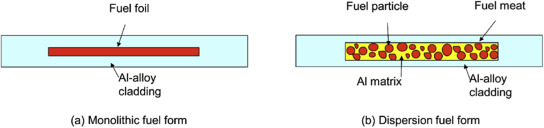
\includegraphics[scale=1.0]{dispersion_monolithic.jpg}
%\caption[Schematic of monolithic and dispersion fuel]{Schematic diagram for monolithic and dispersion fuel from Jeong \etal~\cite{jeong2015mechanical}}
%\end{figure}
 

For five decades, dispersion fuels have powered many test and research reactors worldwide. The manufacturing process and operating conditions are well established for these types of fuels. The high-burnup testing of the dispersion fuel showed a pattern of \mbox{breakaway} swelling~\footnotemark\@ behavior at intermediate burnup. The post-irradiation examination of the U--Mo dispersion fuel revealed that this phenomenon is due to fission gas released from the interaction layer. Reaction between the U--Mo and aluminum occurs during irradiation and forms a ternary [(U--Mo)Al$_x$] phase which releases the fission gas at the boundary between the interaction phase and the aluminum matrix~\cite{leenaers2004post,jue2014microstructural,van2008transmission, olander2009growth}. These gas bubbles have a tendency to aggregate into the gas pockets, which weakens the fuel meat by exerting internal pressure. The result is mechanical failure and increase in fuel volume. To eliminate the fuel--matrix interaction, a `monolithic' U--Mo fuel was suggested. In monolithic fuels, a zirconium foil is used as a diffusion barrier between the fuel and the cladding (aluminum) to prevent diffusion of molybdenum into the cladding~\cite{jue2014microstructural}.

\footnotetext{The \textit{breakaway} is defined as "the limiting exposure, beyond which there will be a marked increase in the rate of swelling as a function of burnup~\cite{osti_10163384}"}

This dissertation investigates how fission gas (xenon and krypton) impacts the transport properties of U--Mo fuel. In Chapter~2 we discuss the reduction of thermal conductivity due to the presence of fission gas. In Chapter~3 we introduce a new pseudopotential for metallic uranium to study the properties using density functional theory (DFT). A basic background of DFT is also discussed in this chapter. In Chapter~4 we look into the diffusion of xenon in \textgamma-uranium and U--Mo alloy. In Chapter~5 we discuss the conclusions and future work.


%In the current work we have investigated how fission gas (xenon and krypton) impacts the U--Mo fuel. In the second chapter we have studied the reduction of thermal conductivity due to the presence of xenon gas. We have implemented finite element method to study the different microstructural configuration of fission gas in U--Mo fuel. In the third chapter we have introduced a new \textit{pseudopotential} for metallic uranium to study the properties using first-principles (Density Functional Theory (DFT)) method. In the fourth chapter we will discuss about the atomistic diffusion mechanism of xenon in U--Mo fuel, which includes the study of xenon gas in the U--Mo fuel using DFT methods. 
















\bibliographystyle{unsrt}
\bibliography{abbreviated,comp}

\chapter{Background}\label{chp:bckgrnd}

\section{First Principles Method}
First principles or \textit{ab initio} methods has become an essential tool in material science over the last three decades. Any relevant physical property of real materials can in principle be described by the law of quantum mechanics. The foundation of this method is computational solution of electronic many-body Schr\"odinger equation. With the proper description of the positions of the atomic nuclei, and the total number of electrons in the system; the energy and other relevant properties can be approximated. The ability to obtain a solution that is good enough, requires well efficient description of electronic system and considerable  computational power.



\subsection{The Many-Body Hamiltonian}
The quantum theory of electrons and nuclei controls the characteristics of matter over wide ranges in temperature and pressure. One of the most fundamental qualities of solid is that it has a variety of properties which are not featured by a single atom. Electric conductivity as well as magnetism arise as collective properties of the particle in the system. The particles of a solid can be described by the Schr\"odinger's equation
\begin{equation}
	\mathcal{H}\ket{\Psi(t)} = i\hbar  \frac{\partial}{\partial t}\ket{\Psi(t)},
\end{equation}
The time-independent Schr\"odinger equation is as follows:

\nomenclature{$\mathcal{H}$}{many body hamiltonian}
\nomenclature{$\Psi(t)$}{time dependent wave function}

\begin{equation}\label{sheqn}
	\mathcal{H}\ket{\psi_j} = E_j\ket{\psi_j}
\end{equation}

where the Hamiltonian expresses the motion of the particles:
\begin{align}\label{hameqn}
 \mathcal{H} &= -\sum_j \frac{\hbar^2}{2m_e}\nabla^2_j - \sum_a \frac{\hbar^2}{2M_a}\nabla^2_a \nonumber \\
			& \quad -\sum_{j,a}\frac{Z_ae^2}{\abs{\vb{r}_j-\vb{R}_a}} + \frac{1}{2}\sum_{j,k}^{j\neq k} \frac{e^2}{\abs{\vb{r}_j - \vb{r}_k}} + \frac{1}{2}\sum_{a,b}^{a\neq b} \frac{Z_aZ_be^2}{\abs{\vb{R}_a - \vb{R}_b}} \nonumber \\
 \mathcal{H} & \stackrel{Htr.\ units}{=} -\sum_j\frac{1}{2}\nabla^2_j - \sum_a\frac{1}{2\tilde{M}_a}\nabla_a^2 \nonumber \\
			& \quad -\sum_{j,a}\frac{Z_a}{\abs{\vb{r}_j - \vb{R}_a}} + \frac{1}{2}\sum_{j,k}^{j\neq k} \frac{1}{\abs{\vb{r}_j-\vb{r}_k}} + \frac{1}{2}\sum_{a,b}^{a\neq b} \frac{Z_aZ_b}{\abs{\vb{R}_a - \vb{R}_b}} \nonumber \\
   & = T_e + T_N \nonumber \\
   & \quad + V_{Ne}(\vb{r},\vb{R}) + V_{ee}(\vb{r}) + V_{NN}(\vb{r}) 
\end{align}

\nomenclature{$m_e$}{mass of a single elctron}
\nomenclature{$\vb{r}_j$}{position of $j$-th electron}
\nomenclature{$\vb{R}_a$}{position of $a$-th nucleus}

The second part of the equation is expressed in Hatree units~(see Appendix~\ref{appen_atomicunit}), which will be used for the remainder of the discussion. In these units, the electron mass $m_e$ as well as the elementary charge $e$, the reduced Planck's constant $\hbar$ and Coulomb's constant $1/4\pi\epsilon_0$ are set to unity, leaving $\tilde{M}_a = M_a/m_e$ as the relative atomic mass of the nucleus of atom $a$. $\vb{r}_j$ denotes the position of the $j$-th electron, while $\vb{R}_a$ is the position of the nucleus of atom $a$. $Z_a$ is that nucleus' charge number. A solution of the Schr\"odinger equation~\eqref{sheqn} would be a function dependent on the spatial coordinates of all particles in the system and is as such only obtainable for very small systems. The Schr\"odinger equation with the above Hamiltonian is impossible to solve exactly for most of systems of interest. A series of approximations and methods were therefore developed to reduce the complexity of the problem. With the help of Eqn~\eqref{hameqn} the Schr\"odinger equation \eqref{sheqn} becomes 

\begin{equation}
 [T_e + T_N + V_{Ne}(\vb{r},\vb{R}) + V_{ee}(\vb{r}) + V_{NN}(\vb{r})]\Phi(\vb{r},\vb{R}) = E\Phi(\vb{r},\vb{R})
\end{equation}
In order to simplify the equations, the electronic coordinates and spin indices are combined into a vector $\vb{r} = (\vec{r},s)$ and $\vb{R}$ denotes the nuclear coordinates. The wave function here is a regular function of the atomic positions but a quantum state $\ket{\Phi(x,t)}$ in the Hilbert space for the electrons and nuclei, so that $\Phi(\vec{r}) = \braket{\vec{r}}{\Phi(\vb{r},\vb{R})}$. The nuclear mass exceeds the electron mass by more than three orders of magnitude, and so both move on different time scales. Thus the wave function $\Phi(\vb{r},\vb{R})$ can be separated into an electronic part $\Psi(\vb{r},\vb{R})$ and a nuclear wave function $\chi(\vb{R})$

\begin{equation}
\Phi(\vb{r},\vb{R}) = \Psi(\vb{r},\vb{R})\chi(\vb{R})
\end{equation}
The nuclear wave function is much more localized, which is why the Schr\"odinger equation can be separated into two parts:
\begin{align}
[T_e + V_{ee}(\vb{r}) + V_{Ne}(\vb{r},\vb{R})]\Psi(\vb{r},\vb{R}) & = \epsilon_n(\vb{R})\Psi(\vb{r},{R})\label{bo1} \\
[T_N + V_{NN}(\vb{R}) + \epsilon_n(\vb{R})]\chi(\vb{r}) & = E\chi(\vb{R})\label{bo2}
\end{align}
The nuclear positions $(\vb{R})$ in the equation~\eqref{bo1} servs only as a parameter and it is possible to use the \textit{adiabatic} or \textit{Born-Oppenheimer} approximation. On the timescale of the nuclar motion the electron follow the ions adiabatically. As a further approximation, the quantum effects on the motion of the nuclei are neglected and time dependent Schr\"odinger equation is replaced by Newton's equation of motion:
\begin{align}
\frac{\partial P_I}{\partial t} & = -\nabla_I E_0 (\vb{R}) \\
with \quad E_0(\vb{R}) & = \epsilon_0(\vb{R}) + V_{NN}(\vb{R})
\end{align}
This refers to the so called \textit{ab-initio} molecular dynamics, where the forces around a nuclei are calculated from the electronic groudn state.

Equation~\ref{bo1} and \ref{bo2} are not generally applicable. However, for several physical systems, the Born-Oppenheimer approximation works and Eqn. ~\ref{bo1}, \ref{bo2} produces meaningful results. In solid state physics, Eqn~\eqref{bo2} usually written in a classical form and Eqn~\eqref{bo1} becomes the problem to be solved. It is still a very complicated equation, where the term describing the interaction between electrons would require the knowledge of $3^N$ variables for a sysmtem of N electrons. Such a large number of variables make the problem computationally not tractable and several approximated methods have been introduced. Some of those important methods will be discussed.

These approximation methods are based on the \textit{independent particle} approximation, in which the Hamiltonian takes the form
\begin{equation}
	\mathcal{H}^{\prime} = \sum_j \mathcal{H}_j
\end{equation}
The electrons wave function can be written as products of single particle wave functions. This leads to a further simplification of the Hamiltonian. 
\begin{align}\label{ham1}
	\mathcal{H}^{\prime} & \stackrel{\text{eqn.} \ref{bo1}} = -\sum_j^N \frac{1}{2}\nabla^2_j - \sum_j^N\sum_a^M \frac{Z_a}{\abs{\vb{r}_j - \vb{R}_a}} + \frac{1}{2}\sum^N_{j\neq k}\sum^N_k\frac{1}{\abs{\vb{r}_j - \vb{r}_k}} \nonumber \\ 
	 &\quad  = T_e + V^{\text{ext}} + \frac{1}{2}\sum_{j\neq k} \upsilon_{jk}(\abs{\vb{r}_j - \vb{r}_k}) 
\end{align}



\subsection{Hartree--Fock Approach}
A very simple way to write many-electron wavefunction is as a product of single-particle wavefunction:
\begin{equation}\label{hwf}
\Psi(r_1,r_2,\dots,r_N) = \prod_j^N \psi_j(r_j)
\end{equation}
The Hamiltonian \eqref{ham1} is not just a sum of single-particle Hamiltonians, the true wavefunctions cannot be written in the product of the form \eqref{hwf}, furthermore, it does not have the \textit{antisymmetry} property required for fermions.

The fermionic nature of the electrons imposes the Pauli exclusion principle as an additional constrant. One can achieve that by constructing a many-body wave function in an antisymmetric manner. This is achieved by writing the electronic wave function as a Slater determinant of single-paricle wave functions:
\begin{equation}\label{hfwf}
\Psi(r_1,r_2,\dots,r_N) = \frac{1}{\sqrt{N!}}\begin{vmatrix}
\psi_1(\vb{r}_1) & \psi_1(\vb{r}_2) & \dots & \psi_1(\vb{r}_N) \\
\psi_2(\vb{r}_2) & \psi_2(\vb{r}_2) & \dots &					\\
\vdots			 &					& \ddots &					\\
\psi_N(\vb{r}_1) & \dots			&		 &  \psi_N(\vb{r}_N) 
\end{vmatrix}
\end{equation}

The expectation value of the Hamiltonian~\eqref{ham1} can be calculated using the newly introduced wave function, which leads to an energy functional that can be minimised variationally~\eqref{vareqn}. Additional constraints for the single particle orbitals is to be normalized~\eqref{norm1}.
\begin{equation}\label{vareqn}
E \le E' \equiv \frac{\bra{\Psi}H\ket{\Psi}}{\braket{\Psi}{\Psi}} = 
\end{equation}
Here, for any state $\ket{\Psi}$ provides an upper bound $E'$ for the exac ground-state energy $E$. The orthonormalization conditions,

\begin{equation}\label{norm1}
\braket{\psi_i(\vb{r}_i)}{\psi_j(\vb{r}_j)} = \int d\vb{r}\ \psi_i(\vb{r})^{\ast} \psi_j(\vb{r}) = \delta_{ij}
\end{equation}
The many-particle wave function~\eqref{hfwf} and the Hamiltonian~\eqref{ham1} give the single particle Hatree-Fock\footnotemark (HF) Equations:
\begin{align}\label{hfeqn}
\begin{split}
\mathcal{H}_i^{\text{HF}} \psi_i(\vb{r}_i) & = \left[-\frac{\nabla^2}{2} + \upsilon^{\text{ext}}(\vb{r}_i) + \upsilon^{\text{H}}(\vb{r}_i) + \upsilon^{\text{EX}}(\vb{r}_i) \right] \psi_i(\vb{r}_i) \\
		& = \epsilon_i\psi_i(\vb{r}_i)
\end{split}
\end{align}
where the kinetic energy term $T_e$ and the external potential $V^{\text{ext}}$ are unchanged from Eqn~\eqref{ham1}, are divided into the single particle constributions, with $V^{\text{ext}} = \sum^N_{i=1}\upsilon^{\text{ext}}(\vb{r}_i)$. The third term in Eqn~\eqref{ham1}, the interaction between the electrons, produces two additional operators $\upsilon^{\text{H}}$ and $\upsilon^{\text{EX}}$. The first term in called the \textit{Hartree potential} and has the following form:
\begin{align}\label{hpot}
\begin{split}
	\upsilon^{\text{H}}(\vb{r}_i) & = \sum_{j=1}^N \int\frac{\abs{\psi_j(\vb{r}_j)^2}}{\abs{\vb{r}_i - \vb{r}_j}} d\vb{r}_j \\
     & = \int \frac{n(\vb{r}_j)}{\abs{\vb{r}_i - \vb{r}_j}} d\vb{r}_j
\end{split}
\end{align}
where
\begin{equation}\label{density}
    n(\vb{r}) = N \int d\vb{r}_1,\dots,d\vb{r}_N \abs{\Psi^0(\vb{r}_1,\dots,\vb{r}_N)}^2
\end{equation}
It takes account of the mean-field Coulomb interaction between the $i$ th electron and the total electron density $n(\vb{r})$ as defined in Eqn~\eqref{hpot}. The second term in Eqn~\eqref{hfeqn} can be written in its integral form
\begin{equation}\label{exeqn}
\upsilon^{\text{EX}}\psi_i(\vb{r}_i) = \sum_{j=1}^N \int d\vb{r}_j\psi^{\ast}_j(\vb{r}_j)\frac{1}{\abs{\vb{r}_i - \vb{r}_j}}\psi_j(\vb{r}_i)\psi_i(\vb{r}_j)
\end{equation}

\nomenclature{$n(\vb{r})$}{electron density}
\nomenclature{$N$}{number of electrons}
\nomenclature{$\upsilon^{\text{EX}}$}{exchange potential}
\nomenclature{$E_{xc}$}{exchange-correlation energy}

It is known as \textit{exchange potential} and takes account the antisymmetric nature of the total wave function. When the two particles have same coordinates the Hatree and exchange potential cancel each other.

The solution of the Hatree-Fock equation are the HF orbitals. Since the orbitals are also part of the equation the problem needs to be solved self-consistently. The exchange operator $\upsilon^{\text{EX}}$ is usually referred to as a non-local operator, which makes it impossible to carry out full HF calculations for condensed matter system without introducing the local approximations. Evaluating $\upsilon^{\text{EX}}$ is already a non trivial task, but the HF equation approximates the full many-body problem in a way that leaves out important contributions. What is not considered is usually referred to as \textit{correlation} which adds an extra term in the Hamiltonian form~\eqref{hfeqn}. This contribution is small compared to the total energy of the system, but it is crucial for many solid systems. The \textit{correlation} contribution to the Hamiltonian takes mainly account of the fact that one electron is screened by others from the interaction with the nuclei and more distant electrons. The HF method is usually works for system in which the particle do not ``see'' each other. HF performs badly for systems with large number of electrons in metals.


\footnotetext{From Hatree~\cite{hartree}, who first postulated the factorization of the wave function in single particle states in 1928, and Fock~\cite{fock}, who redefined the method by including Slater determinant.}


\subsection{Density Functional Theory}
In the Hatree-Fock approach where we used wave-functions to solve many-body problem which is solved self-consistly. The density $n(\vb{r})$ plays a prominent role in self-consistent calculations. This evokes the query as to whether there exists an \textit{exact} theory for the ground state electronic system of the density $n(\vb{r})$. This question leads to the \textit{density functional \mbox{theory}} (DFT). The simplest and oldest version of the DFT formalism is the Thomas-Fermi model\cite{thomas1927calculation,fermi1927metodo}.

\subsubsection{Density}
The idea to shift focus from wavefunction $(\Psi(\vb{r}))$ to denisty $(n(\vb{r}))$ to solve many-body Schr\"odinger equation is very important. For many particle system the density, $n(\vb{r})$, is calculated by the expectatioin value of the single-particle density operator for many-body wavefunction.
\begin{equation}
\hat{n}(\vb{r}) = \sum_i^N \delta(\vb{r} - \vb{r}_i)
\end{equation}
The density can be calculated as follows:
\begin{align}\label{deneqn}
\begin{split}
n(\vb{r}) & = \bra{\Psi}\hat{n}(\vb{r})\ket{\Psi} = \sum_i^N \int \delta(\vb{r}- \vb{r}_i) \abs{\Psi(\vb{r}_1,\dots,\vb{r}_N)}^2\\
    & = N \int \abs{\Psi(\vb{r}_2,\dots,\vb{r}_N}^2
\end{split}
\end{align}
where $\vb{r}_i$ are the variable associated with each of the electrons. Assuming the wavefunction is normalised to unity, the above integration over all the space yields the total number of electrons.
\begin{equation}
	\int d\vb{r} n(\vb{r}) = N
\end{equation} 


\subsubsection{Energy in Terms of the Density}
It is necessary to represent all the energy in terms of density to eliminate wavefunction dependency. This is necessary because the electronic energy needs to be minimized with respect to density to obtain the ground state energy and corresponding electronic density. This is one of the foundations of DFT that was proposed by Hohenberg and Kohn in 1964~\cite{hohenberg1964inhomogeneous}.

As we have discussed earlier (HF theory), once the wavefunction is obtained by solving the Hamiltonian the observable of other operator can be calculated by calculating the expectation value of the operator. This allows to calculate the separate the energy terms associated to the potential operator given in the Hamiltonian~\eqref{ham1}. For the sake of completeness lets reproduce the Hamiltonian in a simplest form
\begin{align}
\begin{split}
\hat{\mathcal{H}}_e &\quad = \quad \hat{T} + \hat{V}_{en} + \hat{V}_{ee} \\
     & \stackrel{eqn. \ref{ham1}}= -\sum_j^N \frac{1}{2}\nabla^2_j - \sum_j^N\sum_a^M \frac{Z_a}{\abs{\vb{r}_j - \vb{R}_a}} + \frac{1}{2}\sum^N_{j\neq k}\sum^N_k\frac{1}{\abs{\vb{r}_j - \vb{r}_k}} 
\end{split}
\end{align}
Lets assume we have managed to solve many-body problem and obtained the wavefunction. The expectation value of the nuclei-electron interaction operator is given by
\begin{align}
\begin{split}
\bra{\Psi(\vb{r}_1,\dots,\vb{r}_N)}\hat{V}_{ne}\ket{\psi(\vb{r}_1,\dots,\vb{r}_N)} &= -\sum_j^N\sum_a^M\Psi^{\ast}(\vb{r}_1,\dots,\vb{r}_N)\frac{Z_a}{\abs{\vb{r}_j - \vb{R}_a}}\Psi(\vb{r}_1,\dots,\vb{r}_N)\\
E_{ne} & = -\sum_a^{M=Nn}\int n(\vb{r})\frac{Z_a}{\abs{\vb{r}-\vb{R}_a}} d\vb{r} \\
       & = \int n(\vb{r})V_{ne}(\vb{r})d\vb{r}
\end{split}
\end{align}

The equivalent derivation for electron-electron term is not trivial. This is because the electron-electron terms require two-particle density instead of single-particle density.
\begin{equation}\label{eeeqn}
E_{ee} = \frac{1}{2}\int\int d\vb{r}d\vb{r}' \frac{n^{(2)}(\vb{r},\vb{r}')}{\abs{\vb{r}-\vb{r}'}}
\end{equation}
where $n^{(2)}$ can be interpreted as the probability of finding an electron at location $\vb{r}$ given that a second electron exists at location $\vb{r}'$. Eqn.~\eqref{eeeqn} makes the many-particle problem so hard to solve. It is required to know the conditional probability $n^{(2)}$ to solve the above equation exactly. However, to make approximation single-particle density is preferred. If the two electrons were complete uncorrelated then two-particle density can be written as the product of one-particle density.
\begin{equation}\label{coreqn1}
n^{(2)} = n(\vb{r})n(\vb{r}') + \Delta n^{(2)}(\vb{r},\vb{r}')
\end{equation}
Where $n^{(2)}$ is a correction term. The electron-electron energy can be written as
\begin{equation}
 E_{ee} = \frac{1}{2}\int\int d\vb{r}d\vb{r}' \frac{n(\vb{r})n(\vb{r})'}{\abs{\vb{r}-\vb{r}'}} + \Delta E_{ee}
\end{equation}
where the $\Delta E_{ee}$ term comes from the correction term in Eqn.~\eqref{coreqn1}.
The kinetic energy operator has a derivative term, which creates a problem to calculate the expectation value. This is because of the derivative, it is not possible to collect wavefunction and its conjugate as a single norm square.
\begin{equation}\label{keeqn}
T = -\frac{1}{2}\int d\vb{r} \Psi^{\ast}(\vb{r}_1,\dots,\vb{r}_N) \nabla^2 \Psi(\vb{r}_1,\dots,\vb{r}_N)
\end{equation}
In order to calculate kinetic energy the key assumptions of DFT is to expand the density as the sum of squares of single-particle orbitals
\begin{equation}
n(\vb{r}) = \sum_j^{N_e} \abs{\phi_j(\vb{r})}^2
\end{equation}
These orbitals are called \textit{Kohn-Sham} orbitals. Now the kinetic energy term can be written as single-particle kinetic energy plus a correction
\begin{equation}
T = -\frac{1}{2}\sum_j^{N_e} \int d\vb{r} \phi^{\ast}_j (\vb{r})\nabla^2 \phi_j(\vb{r}) + \Delta T
\end{equation}
The total ground state energy can be written as
\begin{equation}
\begin{split}
E  & = -\frac{1}{2}\sum_j^{N_e} \int d\vb{r} \phi^{\ast}_j (\vb{r})\nabla^2 \phi_j(\vb{r}) + \int n(\vb{r})V_{ne}(\vb{r})d\vb{r} +  \frac{1}{2}\int\int d\vb{r}d\vb{r}' \frac{n(\vb{r})n(\vb{r})'}{\abs{\vb{r}-\vb{r}'}} + \Delta E_{ee} + \Delta T \\
   & =-\frac{1}{2}\sum_j^{N_e} \int d\vb{r} \phi^{\ast}_j (\vb{r})\nabla^2 \phi_j(\vb{r}) + \int n(\vb{r})V_{ne}(\vb{r})d\vb{r} +  \frac{1}{2}\int\int d\vb{r}d\vb{r}' \frac{n(\vb{r})n(\vb{r})'}{\abs{\vb{r}-\vb{r}'}} + E_{xc}
\end{split}
\end{equation}
Here the two correction terms are replaced with $E_{xc}$, called the \textit{exchange-correlation} energy. The origin of this term is the difference between $N$ interacting and noninteracting particles. Several well-developed approximations exist for exchange-correlation, and one of them is called local approximation
\begin{equation}\label{ldaeqn}
E_{xc} = \int d\vb{r} n(\vb{r})\epsilon_{xc}([n],\vb{r})
\end{equation}
where $\epsilon_{xc}$ is an energy per electron at point $\vb{r}$ that depends only on the density $n(\vb{r})$. Thus, within the local density approximation the total energy can be written as
\begin{align}\label{toteeqn}
\begin{split}
E=-\frac{1}{2}\sum_j^{N_e} \int d\vb{r} \phi^{\ast}_j (\vb{r})\nabla^2 \phi_j(\vb{r}) + \int n(\vb{r})V_{ne}(\vb{r})d\vb{r}  \\
+ \frac{1}{2}\int\int d\vb{r}d\vb{r}' \frac{n(\vb{r})n(\vb{r})'}{\abs{\vb{r}-\vb{r}'}} + \int d\vb{r} n(\vb{r})\epsilon_{xc}([n],\vb{r})
\end{split}
\end{align}
The above equation is used to derive to obtain Kohn-Sham equation which makes DFT applicable in practice. The functional form of the above equation can be written as follows:
\begin{equation}
E_{\text{KS}}[n] = T_s[n] + \int d\vb{r} V_{\text{ext}}n(\vb{r}) + E_{\text{H}}[n] + E_{\text{xc}}[n]
\end{equation}
Here $V_{\text{ext}}$ is the external potential due to the nuclei and other external field.
\nomenclature{$V_{\text{ext}}$}{external potential}
\nomenclature{$E$}{energy of the system}


\subsection{Kohn--Sham Equations}
The previous section addressed the formation of K-S equation and the idea of self-consistency. In DFT based calculation, methods are classified based on the representation of the density, potential and especially KS orbitals. The choice of representation is made to increase the computational efficiency, while maintaining the accuracy.
For a choice of basis, the coefficients are the only variable to be determined (density depends on KS orbitals). The total energy of DFT becomes variational, then the solution of the self-consistent KS equations requires to determine occupied orbitals that provides a minima of the total energy.

According to the second theorem of Hohenberg and Kohn, all properties such as kinetic energy, etc. are uniquely determined if $n(\vb{r})$ is specified. Eqn~\eqref{toteeqn} shows the relationship. To minimize the total energy with respect of KS orbitals, the variational principle is usually used. While performing the minimization, it is prefer to minimize with $\phi^{\ast}(\vb{r})$ (both yield the same result). Using the chain rule for functional derivatives, the equations becomes:
\begin{equation}
\label{eq_var_ks}
\frac{\delta E}{\delta \phi^{\ast}_i(\vb{r})} = \frac{\delta T_s}{\delta \phi^{\ast}_i(\vb{r})} + \left [ \frac{\delta E_{\text{ext}}}{\delta n(\vb{r})} + \frac{\delta E_H}{\delta n(\vb{r})} + \frac{E_{xc}}{\delta n(\vb{r})}	\right ] \frac{\delta n(\vb{r})}{\delta \phi^{\ast}_i(\vb{r})}  = 0
\end{equation}
The kinetic energy may be differentiated separately with respect to orbital. In the above equation the $E_{ei}$ is replaced with $E_{ext}$ which means potential due to nuclei and any other external fields.
\begin{equation}
\label{eq_var_ks_eig}
-\frac{1}{2} \nabla^2 \phi^{\ast}_i (\vb{r}) + \left [ V_{\text{ext}} (\vb{r}) + \int d(\vb{r'}) \frac{n(\vb{r'})}{\abs{\vb{r}-\vb{r'}}} + \epsilon_{xc} (n) + n(\vb{r}) \frac{\delta \epsilon_{xc}[n]}{\delta n(\vb{r})}   \right ] \phi_i(\vb{r})  = \epsilon_i \phi_i (\vb{r})
\end{equation}
Eqn~\ref{eq_var_ks_eig} is a system of equations, represent the many-particle system in terms of single-particle orbitals. Each of these equations resemble a \schrod equation.
\begin{equation}
\label{eq_ks_s}
\left [ \hat{T} + V_{eff}\right ] \phi_i (\vb{r}) = \epsilon_i \phi_i (\vb{r})
\end{equation}

%Deriving Eqn~\ref{eq_var_ks_eig} from Eqn~\ref{eq_var_ks} involves variational principle and using Lagrange multiplier for \schrod equation. 
Here the $V_{eff}$ is the sum of the $V_H$, $V_{xc}$ and $V_{\text{ext}}$, which depends on the density and indirectly depends on orbitals. Now we have an equation where any change in the orbitals effect also the potential on which they in turn depend on orbital. This problem is resolved by solving Kohn-Sham system of equations self-consistently.
\begin{center}
\begin{figure}
\begin{tikzpicture}[node distance =2 cm, auto]
	\node [block] (inguess) {Initial guess};	
	\node [block] (inguess2) [below of =inguess, yshift=0.75 cm] {$n(\vb{r})$};
	\node [block2] (cal1) [below of = inguess2] {Calculate effective potential};
	\node [block2] (cal2) [below of =cal1, yshift = 0.75 cm] {$V_{eff}(\vb{r}) = V_{\text{ext}} (\vb{r}) + V_H[n] + V_{xc} [n]$};
	\node [block2] (sol1) [below of = cal2] {Solve KS equations};
	\node [block2] (sol2) [below of = sol1, yshift = 0.75 cm] {$\left [-\frac{1}{2} \nabla^2 + V_{eff}(\vb{r}) \right] \phi_i(\vb{r}) = \epsilon_i \phi_i(\vb{r})$};

	\node [block2] (den1) [below of = sol2] {Calculate electron density};
	\node [block2] (den2) [below of = den1, yshift = 0.75 cm] { $n(\vb{r}) = \sum_{\alpha} c_{i\alpha} \abs{\phi_i(\vb{r})^2}$ };

	\node [decision] (slf) [below of = den2, yshift = -1.3 cm] {Self-consistent ?};
	\node [block3] (result) [below of = slf, yshift = -1.3 cm] {Output Quantities};
	\node [block3] (resultfin) [below of = result, yshift = 0.73 cm] {Energy, forces, stresses, eigenvalues...};


	\path [line] (inguess2) -- (cal1);
	\path [line] (cal2) -- (sol1);
	\path [line] (den2) -- (slf);
	\path [line] (sol2) -- (den1);
	\path [line] (slf) -- node {yes} (result);
	\draw[thick, ->] (slf.west) -- node {no} ++ (-5, 0.0cm) |- (inguess2) ;
\end{tikzpicture}
\caption{Schematic representation of the self-consistent loop solution of Kohn-Sham equations.}
\end{figure}
\end{center}

\subsection{Kohn--Sham problem for an isolated atom}
For an one-electron atom, the Coulombic potential, $V(\mathbf{r}) = V(r) = -Z/r$ is spherically symmetric, the solution can be split into a radial and an angular part 
\begin{equation}
\label{eq_rad_ang}
\psi_{n\ell m} (\mathbf{r}) = \psi_{n\ell}(r) Y_{\ell m}(\theta,\phi) = r^{-1} \phi_{n\ell}(r) Y_{\ell m} (\theta,\phi)
\end{equation}

\nomenclature{$n$}{principle quantum number}
\nomenclature{$\ell$}{angular quantum number}
\nomenclature{$m$}{spin}


The above equation sometime is referred to as spherically symmetric \schrod equation and $Y_{\ell m}(\theta, \phi)$ are normalized spherical harmonics. Using the Laplacian in the spherical coordinates the wave equation can be reduced to the radial equation for principle quantum number n
\begin{equation}
\label{eq_radial}
-\frac{1}{2}\frac{d^2}{dr^2} \psi_{n\ell} + \left [ \frac{\ell(\ell+1)}{2r^2} + V_{ext}(r) - \epsilon_{n\ell} \right ] \psi_{n\ell} = 0
\end{equation}
In the Kohn-Sham approach to the many-particle system, the form of the single-particle equations are identical to the above radial \schrod equation with an effective potential $V_{eff}$ replacing the Coulomb potential. The effective potential $(V_{eff} = V_{ext}(r) + V_{H} (r) + V_{xc} (r))$ is spherically symmetric in the Kohn-Sham approach. The independent-particle Kohn-Sham states may be classified by the angular quantum numbers L = \{$\ell$, m\}, and the one particle equations becomes analogous to the \schrod equation for one-electron atom. 
\begin{equation}
\label{eq_oneparticle}
-\frac{1}{2}\frac{d^2}{dr^2} \psi_{n\ell} + \left [ \frac{\ell(\ell+1)}{2r^2} + V_{eff}(r) - \epsilon_{n\ell} \right ] \psi_{n\ell} = 0
\end{equation}

\subsection{Theory of Pseudopotential}
In Solids, the electrons and nuclei interact strongly through the Coulomb potential. However, according to the Fermi Liquid theory (FLT) the electronic excitation near the Fermi energy in metals behave as if they were independent particles. This leaves the strong interactions with the core electrons and the nuclei. In most cases, the core electrons are quite strongly bound, and do not respond effectively to the motions of the valence electrons. Hence, they can be regarded as essentially fixed.
\begin{figure}
\centering
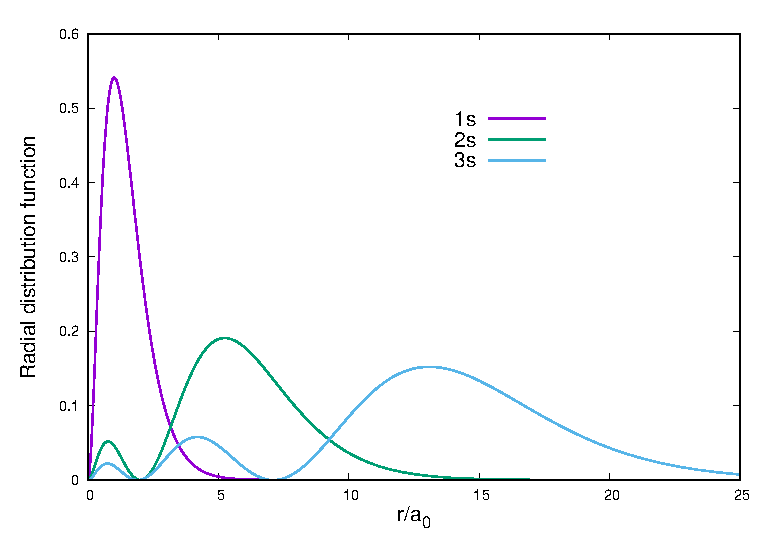
\includegraphics[scale=0.8]{radialdistfuncS.eps}
\caption{Radial distribution function of Hydrogenic 1s, 2s and 3s electron. It shows higher kinetic energy near the nucleus.}
\label{fig_hydrogen}
\end{figure}
This is the essence of the pseudopotential approximation, the strong core potential is replaced by a pseudopotential, whose ground state wave function resembles the all electron wavefunction outside a selected core radius. In this way both the core states and the wiggles (Fig.~\ref{fig_hydrogen}) in the valance wavefunctions are removed. For many metals the pseudowavefunctions can be represented by lower number of planewaves. Thus making planewaves a simple and reasonable efficient basis for the pseudo wavefunctions.
\begin{figure}
\centering
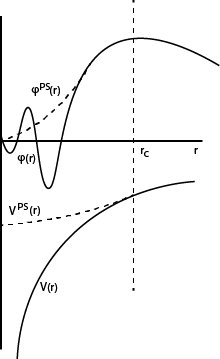
\includegraphics[scale=0.80]{pseudo_figure_01.png}
\caption{Schematic diagram of the replacement of all-electron wave function and core potential by a pseudo-wavefunction and pseudopotential.}
\end{figure}
\subsection{Basic Phillips--Kleinman Construction}
For a given many electron Hamiltonian, $\hat{H}=\hat{T}+\hat{U}$, where $\hat{T}$ is the kinetic energy operator and $\hat{U}$ is the potential energy operator, the core electron wave functions are defined by the \schrod equation
\begin{equation}
 \hat{H}\ket{\psi_i} = \epsilon_i \ket{\psi_i} \quad   (i = 1, n core)
\end{equation}

The valance electron wave function similarly can be found by the Hamiltonian
\begin{equation}
\label{eq_val_hamil}
\hat{H}\ket{\psi_{\upsilon}} = \epsilon_{\upsilon} \ket{\psi_{\upsilon}}
\end{equation}
The valence electron wave function is orthogonal to the core electron wave function ($\braket{\psi_{\upsilon}}{\psi_i}=0$), this orthogonality always has to be preserved, even if the core electrons are not treated explicitly. One way to preserve this orthogonality is to write valence electron wave function in a basis set that is priori orthogonal to the core electrons. The simple Gram-Shmidt orthogonalization technique can be used. Herring~\cite{herring1940new} was the first one to use Orthogonalized plane waves (OPWs)(Appendix~\ref{appen_opw}) as basis for the first quantitative calculations of bands. Using this idea, we can orthogonalize any arbitrary basis set $\{\ket{\chi_n}\}$ to the core electron wave functions by defining a new basis set $\{\ket{\varrho_n}\}$

\begin{equation}
\label{eq_pk}
\ket{\varrho_n} = \ket{\chi_n} - \sum^{ncore}_{i=1} \braket{\psi_i}{\chi_n}\ket{\psi_i}
\end{equation}
Here each of the new basis set, $\{\ket{\varrho_n}\}$, satisfies $\braket{\chi_n}{\psi_i} = 0$ for each $\ket{\psi_i}$. Now we can express the valance electron wave function as a linear combination of the new basis sets,
\begin{equation}
\label{eq_val}
\ket{\psi_{\upsilon}} = \sum_n C_n \ket{\varrho_n} 
\end{equation}
Using Eqn~\ref{eq_pk} into the Eqn~\ref{eq_val}, the valence electron can be expressed in the following way. The orthogonality condition with the core electron still valid.
\begin{equation}
\ket{\psi_{\upsilon}} = \sum_n C_n \left [ \ket{\chi_n} - \sum_{i=1}^{ncore} \ket{\psi_i}\braket{\psi_i}{\chi_n} \right ] = \ket{\phi} - \hat{\Omega}\ket{\phi}
\end{equation}
Here, $\hat{\Omega}$ is a projection operator for core electron wave function
\begin{equation}
\label{eq_projection}
\hat{\Omega} = \sum_{i=n}^{ncore} \dyad{\psi_i}{\psi_i}
\end{equation}
and a new wave function which is a linear combination of $\ket{\chi_n}$, sometime designated as pseudo-orbital,
\begin{equation}
\label{eq_pseudoorbital}
\ket{\phi} = \sum_n C_n \ket{\chi_n}
\end{equation}
This technique of representing the valance electron wave function in preorthogonalized basis set has been studied and used as a computational tool~\cite{herring1940new}. It took the insight of the Phillips and Kleinman~\cite{phillips1959new}. The new pseudoorbitals satisfies the orthogonality condition, but it also change the Hamiltonian so that the eigen values are same with the valance electrons. Mathematically, it can be obtained by replacing original valance electron Hamiltonian equation (Eqn~\ref{eq_val_hamil}) with newly obtained pseudo wave function.
\begin{equation}
\label{eq_ps_pot}
\hat{H}\ket{\psi_{\upsilon}} = \hat{H} \left [ \ket{\phi} - \sum_n \ket{\psi_i}\braket{\psi_i}{\phi} \right ] =\epsilon_{\upsilon} \left [ \ket{\phi} - \sum_n \ket{\psi_i}\braket{\psi_i}{\phi}  \right ] 
\end{equation}
Rearranging the above equation provides a new Hamiltonian,
\begin{equation}
\label{eq_ps_hamil}
\left [ \hat{H} + \sum_n ^{ncore} (\epsilon_{\upsilon} - \epsilon_i)\ket{\psi_i}\bra{\psi_i}\right ]\ket{\phi} = 
\epsilon_{\upsilon}\ket{\phi}
\end{equation}
The above equation has the form of the original valance electron eigenequation (\ref{eq_val_hamil}), but with an extra term for preorthogonalization. This extra potential $(V_{nl} = \sum_n^{core} \dyad{\psi_i}{\psi_i})$, is a nonlocal operator, and the pseudo orbital $(\ket{\phi)}$ is an eigenstate of the new effective Hamiltonian, $\hat{H} + V_{nl}$. The new Hamiltonian has an extra potential $V_{nl}$, which depends on the angular momentum $l$ due to the spherical symmetry. Because of its spherical symmetry, each angular momentum $l$, $m$ can be treated separately. The dependence on $l$ means that, a pseudopotential is an non-local operator, can be written in ``semilocal'' (SL) form
\begin{equation}
\label{eq_sl}
\hat{V}_{SL} = \sum_{\ell m} \ket{Y_{\ell m}}V_\ell(r)\bra{Y_{\ell m}}
\end{equation}
Where $Y_{\ell m}(\theta,\phi) = P_\ell(cos(\theta))e^{im\theta}$. It is semi-local because it is non local on the angular variables but local in the radial variable.\footnote{$P_l$ is the Legendre polynomials}


The sophistication and accuracy have evolved considerably since the Phillips-Kleinman construction. This development produces many methods of generating pseudopotentials. All of these methods follow these goals: (1) Pseudopotential should be as soft as possible, so that it can allow representation of pseudo-wavefunction with fewer planewaves. (2) Transferability has to be maintained (it means a generated pseudopotential with a configuration should produce other properties accurately) (3) the pseudo-charge density should produce the valance charge density as accurately as possible. 


\subsection{Norm-Conserving Pseudopotentials}
Hamann, Schl\"uter and Chiang~\cite{hamann1979norm} developed the concept of norm-conservation, which was a first step to fulfill all the above requirements. As the exchange-correlation energy of the electronic system depends on the electron density, it is necessary that outside the core region the real and pseudo wavefunctions be indentical. In the outer region ($r > r_c$), both functions coincide. Threfore, the total charge density created in the core region $(r < r_c)$ must be the same after pseudisation:
\begin{equation}
\int^{r_{c}}_0 \psi^{\ast}_{AE}(r)\psi_{AE}(r)dr = \int^{r_c}_0 \psi^{\ast}_{ps}(r)\psi_{ps}(r)dr
\end{equation}

\nomenclature{$\psi_{AE}$}{all electron wave function}
\nomenclature{$\psi_{ps}$}{pseudo wave function}


Where $\psi_{ae}(r)$ is the all electron wavefunction and $\psi_{ps}$ is the pseudo wavefunction. The logarithmic derivatives of the real and pseudo wave function and their energy derivative agree in the outer region. These types of pseudopotentials are the most transferable since they are able to reproduce the scattering properties of an ion in different chemical environments\cite{hamann1979norm}. The downsize of Norm-Conserving pseudopotenttial is a higher cutoff radiuss and thus increased memory and CPU requirements. Troullier and Martins~\cite{troullier1991efficient} developed a more effective method to generate norm-conserving pseudopotentials for practical calculations. 

\subsection{Ultrasoft Pseudopotentials}
The norm conservation requirement produces a very high requirement of cutoff energy for the plane-wave basis set. Particularly the tightly bound orbitals that have a substantial fraction of their weight inside the core region of the atom. There are some important cases where it was impossible to construct a pseudopotential that allows a significant reduction of the cutoff energy. Vanderbilt~\cite{vanderbilt1990soft} suggested to relax the norm conservation criteria in favor of a smoother (i.e. softer) potential. The ultrasoft pseudopotentials are difficult to construct and require extensive testing~\cite{kresse1999ultrasoft}.

\subsection{Projector Augmented-Wave Method (PAW)}
The electronic wave functions oscillate wildly near the nuclei (Fig.~\ref{fig_hydrogen}) than the bonding area between the atoms. Expanding these region using plane-wave creates computational challenges. Augmented-wave methods uses the separation of the wave functions in two regions to address this issue. The first part is partial wave expansion inside an atom-centered sphere called the augmentation region and a plane wave expansion outside. Both expansions are continuously differentiable at the boundary.

Bl\"ochl~\cite{Bloechl1994} suggested that there is a linear transformation from the all-electron to the pseudo wave functions. The transformation is as follows:
\begin{equation}
\ket{\Psi} = \ket{\tilde{\Psi}} + \sum_i (\ket{\phi_i} - \ket{\tilde{\phi_i}})\braket{\tilde{p_i}}{\tilde{\Psi}}
\end{equation}
Here $\phi_i$ are the partial waves within the augmentation regions, and $\bra{\tilde{p_i}}$ is a projector with a condition of $\braket{\tilde{p_i}}{\tilde{\phi_i}} = \delta_{ij}$. The tilde quantities are related the pseudo representation. Kresse and Joubert~\cite{kresse1999ultrasoft} showed a connection between PAW and US-pp and how the PAW method can be implemented into existing code.



\bibliographystyle{apsrev4-1}
\bibliography{abbreviated,comp}


%\chapter{Effect of Xenon on the overall thermal conductivity of \protect\NoCaseChange{U--{10}Mo}}
\chapter{Estimation of Effective Thermal Conductivity in \protect\NoCaseChange{U-10Mo} fuels with distributed xenon gas bubbles}
\textit{This chapter was published as an article in the \textup{Journal of Nuclear Materials}. The authors of that article are A. Rafi M. Iasir and Karl D. Hammond of the University of Missouri and Nickie J. Peters of the University of Missouri Research Reactor Center.}

\section{Introduction}\label{sec:introduction}
The Reduced Enrichment for Research and Test Reactors (RERTR)~\cite{snelgrove1997development} program was initiated in the USA in the late 1970s to develop new nuclear fission fuels to replace high-enrichment uranium (HEU)\@. The development of low-enrichment uranium (LEU) fuels for high-performance reactors is an important nonproliferation initiative~\cite{snelgrove1997development}. One of the main requirements of LEU fuels is increased uranium density, such as that found in metallic uranium, to offset the decrease in \textsuperscript{235}U enrichment. Metallic uranium is thought to have sufficient density, but the orthorhombic crystal structure of \textalpha-uranium
and the anisotropic fuel swelling that results make it unattractive as a fuel.
Uranium alloys that retain the high-temperature \textgamma-phase, which is body-centered cubic, are more suitable for reactor fuel due to their more isotropic radiation-induced swelling behavior compared with  \textalpha-uranium~\cite{kittel1993history}.

Various uranium alloys have been tested as alternative metallic fuels under reactor operating conditions, including U$_6$Fe and U$_6$Mn~\cite{meyer2000irradiation,hofman1987irradiation}.
%The U-Mo alloy has been identified as a high-performance fuel due to its high uranium density and low neutron capture cross-section~\cite{ewh2010microstructural,smirnova2013ternary,rest2009analysis,landa2013density}.
Elements such as molybdenum (Mo), niobium (Nb), titanium (Ti), and zirconium (Zr) have also been tried as alloying elements because of their solubility in \textgamma-uranium~\cite{donze1959stabilisation,giraud1973formation,lopes2013mechanical}. Molybdenum stabilizes uranium's \textgamma-phase at concentrations near the eutectoid point, lowering the phase transition temperature from 776~\textdegree C for pure uranium (corresponding to the \textbeta--\textgamma\ allotropic point) to the eutectoid point of 555~\textdegree C for 11.1~percent molybdenum in \textgamma-uranium by weight~\cite{ASM-Alloy-Mo,Berche2011}. To take advantage of this, uranium alloyed with 10 wt$\%$ molybdenum (U-10Mo) is currently being developed as a potential high-density LEU fuel for high-performance research reactors.

The two major fuel types are U--Mo/Al dispersion fuels (U--Mo grains dispersed in an aluminum matrix) and U--Mo monolithic fuels~\cite{keiser2012effects}. Dispersion fuels show poor irradiation performance due to fuel--matrix interaction, which causes break-away swelling behavior at intermediate burnup~\cite{hofman2004post,van2008transmission, leenaers2004post}. In monolithic fuels, a zirconium foil is used as a diffusion barrier between the fuel and the cladding (aluminum) to prevent diffusion of molybdenum into the cladding~\cite{jue2014microstructural}.

Thermal conductivity is an important property of any nuclear fuel, since most of the important physical properties are temperature-dependent. In the case of high-performance reactors, fuels must undergo high fission density at relatively low temperatures. For this reason, research reactor fuels are designed for efficient heat rejection. During test operations, Burkes and coworkers~\cite{burkes2015thermal} observed that the thermal conductivity in monolithic fuels decreased significantly with increased burnup. For a fission density of $3.30\times10^{21}$~fissions/cm$^3$ at 200~\textdegree C, thermal conductivity decreased by approximately 30\%; at $4.53\times10^{21}$~fissions/cm$^{3}$, conductivity decreased by 45\%~\cite{burkes2015thermal}.

Fission also creates a variety of fission products, which result in gas
bubbles, metallic precipitates, and solutes in the fuel
matrix~\cite{rondinella2010high}. These fission products, in addition to
radiation damage in reactor environments, result in complex microstructural
evolution that restructures the nuclear fuel over time. Fission gas bubbles are
particularly problematic, as they cause changes in thermal conductivity and
swelling of the fuel. In addition, \textsuperscript{135}Xe is a potent neutron
absorber. {Solid fission products (e.g., Sr, Y, Zr, La, Ce,
and Nd)\ are also constantly being produced; these elements can form
intermetallic alloys, which can increase the volume of the fuel and reduce the
thermal diffusivity~\cite{ishimoto1994effects, kang2007thermal}. These solid
fission products also play an important role in the thermal stability of
fission gas bubbles~\cite{gan2015thermal}.} 

For every four fission events, an average of one inert gas atom (xenon or krypton) is produced. The dominant gaseous species is xenon, accounting for almost $85\%$ of fission gas~\cite{blades1956ratio,petruska1955absolute}. Xenon atoms in U--Mo alloy fuels have a strong tendency to precipitate into small bubbles due to their low solubility. The formation and growth of gas bubbles inside irradiated nuclear fuels has technical importance, as bubbles influence the microstructure of the material~\cite{kim2011fission}. Recent TEM and SEM images show that fission bubbles in U-10Mo distribute themselves in both inter-granular and intra-granular formations~\cite{miller2015transmission,miller2012advantages, gan2012tem, gan2010transmission}. High-fission-density fuels show randomly-distributed, micrometer-sized fission gas bubbles distributed throughout the grains~\cite{gan2012tem}. Inter-granular bubble density increases with burnup. 

Inside the micrometer-sized grains, fission gas forms superlattices~\cite{miller2015transmission,miller2012advantages, gan2012tem},
similar to those seen in ion-irradiated materials~\cite{johnson1980gas, johnson1980hydrogen, evans1983void, mazey1986bubble, evans1986solid, johnson1991image, johnson1995gas, lawson1998temperature, ghoniem2001theory,johnson2006helium}. Typical bubble sizes are 2--6~nm in diameter, and the distance between the bubbles is typically in the 4--12 nm range. The superlattice usually has the same crystal structure as the host material, but an exception exists: the superlattice in U-10Mo shows a face-centered cubic structure in a body-centered cubic matrix. An ion-irradiated bubble superlattice has a lattice parameter of tens of nanometers~\cite{miller2015transmission}; that of fission gas bubbles is
typically similar~\cite{Gan2015}.
The superlattice forms in ion-irradiated materials between approximately
$0.15T_m$ and $0.35T_m$~\cite{lawson1998temperature}, which is within the
typical anticipated operating range of \mbox{U--Mo} fuels, and the superlattice
in \mbox{U-10Mo} can survive temperatures up to approximately
850~\textdegree C~\cite{Gan2015}.

The thermal conductivity of a monolithic \mbox{U--Mo} fuel plate is at a maximum prior to irradiation~\cite{burkes2015thermal}.
Inclusions and porosity change the thermal and the electrical conductivity of many materials~\cite{bakker1997using}. 
Solid fission products usually have minimal impact on overall thermal conductivity, as their conductivities are similar to the conductivity of the fuel. Gases, on the other hand, have much lower thermal conductivity than
the matrix, and typically have much lower densities and heat capacities as well. Various models, both empirical and theoretical, have been proposed to describe the changes in conductivity due to gas bubbles. Maxwell~\cite{maxwell1881treatise} was among the first to derive an expression for the effective thermal conductivity of heterogenic media; his model assumed a uniform distribution of spherical particles in a matrix. A few other empirical models also exist~\cite{macewan1967effect,goldsmith1973measurements,devries1989experimental}; unfortunately, the large diversity of pore shape, pore size, and type of included material inside nuclear fuel make it impossible to describe heat transfer with a single equation. Several theoretical models have been proposed to describe the influence of porosity and inclusions on the thermal conductivity~\cite{maxwell1881treatise,loeb1954thermal, cunningham1981heat, tzou1991effect, bauer1993general}. These theoretical models usually assume pores with regular geometric shapes and that the pore arrangement is sufficiently dilute so as to neglect interaction between inclusions.

The microstructure of irradiated nuclear fuels is very complicated due to the lack of consistency between bubbles. The intra-granular gas bubbles are two or three orders of magnitude smaller than the inter-granular gas bubbles~\cite{hu2015assessment}. The shapes of the bubbles are also highly variable: the intra-granular gas bubbles are approximately spherical, whereas inter-granular gas bubbles do not have consistent shapes. In this work, we assess contributions to the thermal conductivity of \mbox{U-10Mo} from both inter- and intra-granular gas bubbles. The impact of xenon bubble pressure on the overall thermal conductivity is also estimated.
{Because fission gas is typically a mixture of krypton and
xenon, rather than pure xenon, we include two comparisons with a krypton--xenon
mixture.}
At the end, we present a study of the influence of different bubble arrangements on the overall thermal conductivity.

 

\section{Methods} \label{sec:Methodology}
A finite element model was used to solve the steady-state heat conduction equation in the presence of various microstructures. Two types of microstructures containing xenon gas bubbles were used: a xenon bubble superlattice structure representing intra-granular bubbles, and a grain boundary structure representing inter-granular bubbles. Figure~\ref{gbs} shows an example of an intra-granular bubble distribution, while Figure~\ref{fig_Xe_SEM} shows the inter-granular bubble distribution.
In the intra-granular bubble case, xenon gas bubbles were placed in a variety
of spatial configurations, including configurations consistent with a gas bubble superlattice.
\begin{figure}%[H]
    \centering
	  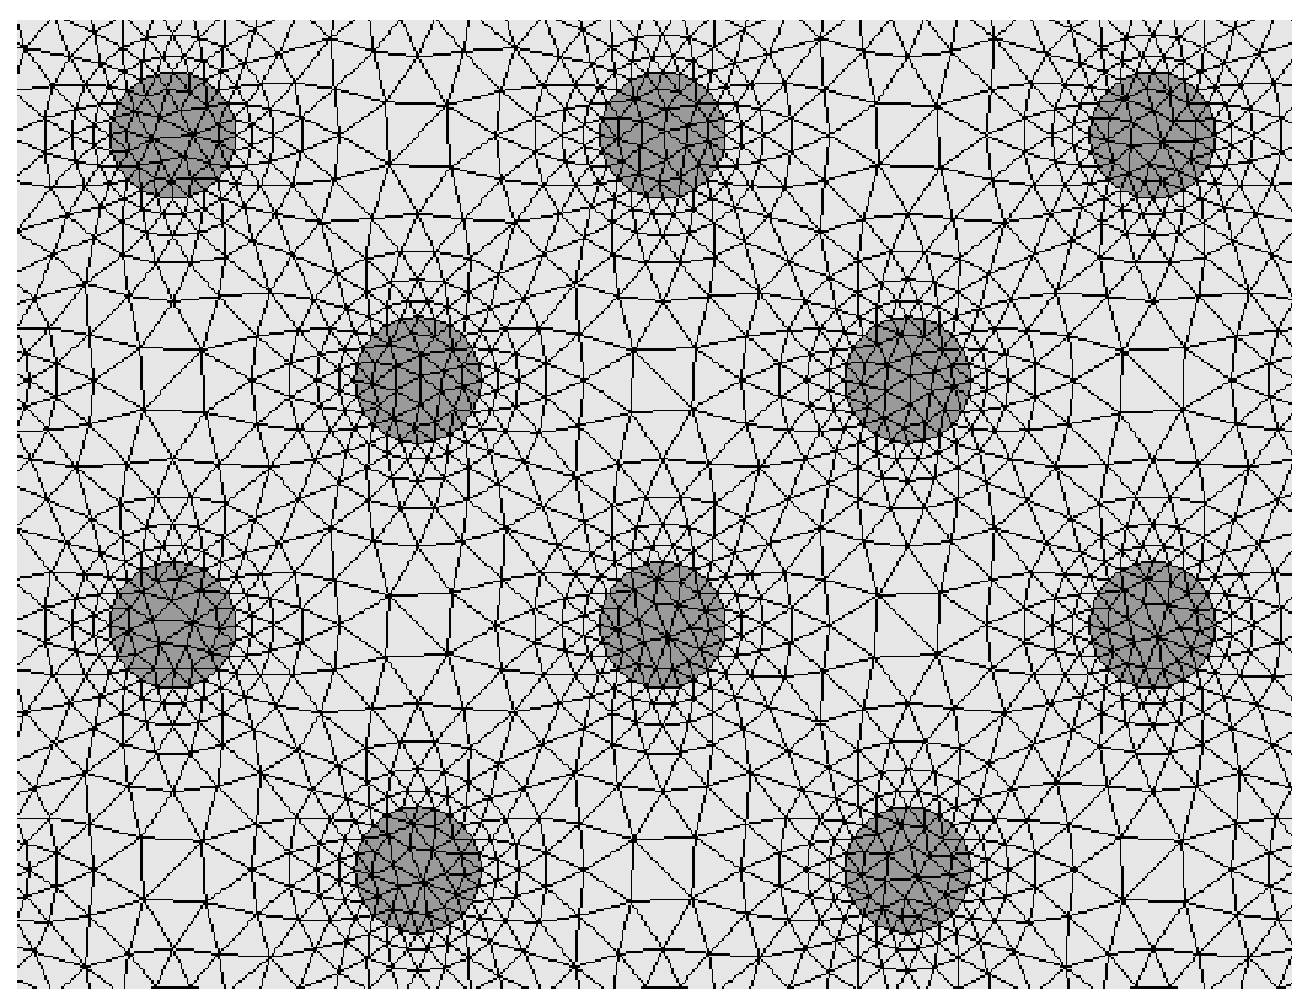
\includegraphics[width=3.25in]{meshed_figure_GBS_gray}
    \\
	 
\includegraphics[width=3.25in]{figure_GBS_fcc_2_gray}
	\caption[(a)~Discretized domain of intra-granular xenon bubbles inside a U-10Mo matrix; (b)~Example two-dimensional bubble distribution 
used for intra-granular xenon gas, consisting of bubbles with 3.1, 3.6, 3.75,
        and 4.0~nm diameters, consistent with the work of Miller and
        coworkers]{(a)~Discretized domain of intra-granular xenon bubbles inside a U-10Mo matrix; (b)~Example two-dimensional bubble distribution 
used for intra-granular xenon gas, consisting of bubbles with 3.1, 3.6, 3.75,
        and 4.0~nm diameters, consistent with the work of Miller and
        coworkers~\cite{miller2015transmission}. The lattice parameter for the
        gas bubble superlattice is 12.0~nm.}
	\label{gbs}
\end{figure}
All simulations were performed in a two-dimensional domain. The gas bubble supperlattice structure was created based on data from Miller \etal~\cite{miller2015transmission}. According to Miller \etal~\cite{miller2015transmission}, the bubble size inside the grain boundary superlattice structure is normally distributed. Based on their experimental values, we chose four bubble diameters to create our simulation. Because the superlattice in U-10Mo is FCC, the two-dimensional structure of bubbles was created based on the FCC structure with a 12~nm lattice parameter, which was also taken from Miller \etal~\cite{miller2015transmission}. The bubble sizes were randomly sampled from this distribution using the discrete values of 3.1, 3.6, 3.75, and 4.0~nm in diameter. The square domain's dimensions were 80~nm${}\times{}$80~nm, which results in 85 bubbles with a lattice constant of 12~nm. Triangular elements were used to create the mesh using the Trelis Pro software package~\cite{trelis}.

In the inter-granular bubble case, the grain boundary structure of U-10Mo was created based on images from Miller \etal~\cite{miller2012advantages}. Their SEM (scanning electron micrograph) of a focused ion beam (FIB) cross-section showed fission gas bubbles populating the grain boundaries, as shown in Figure~\ref{fig_Xe_SEM}. This domain was also discretized with triangular elements. The top and bottom boundaries of the domain of the FEM domain were assumed to be adiabatic. The left and right boundaries have fixed-temperature boundary conditions applied. This temperature difference drives the heat flow. 


\begin{figure}%[t]
\centering
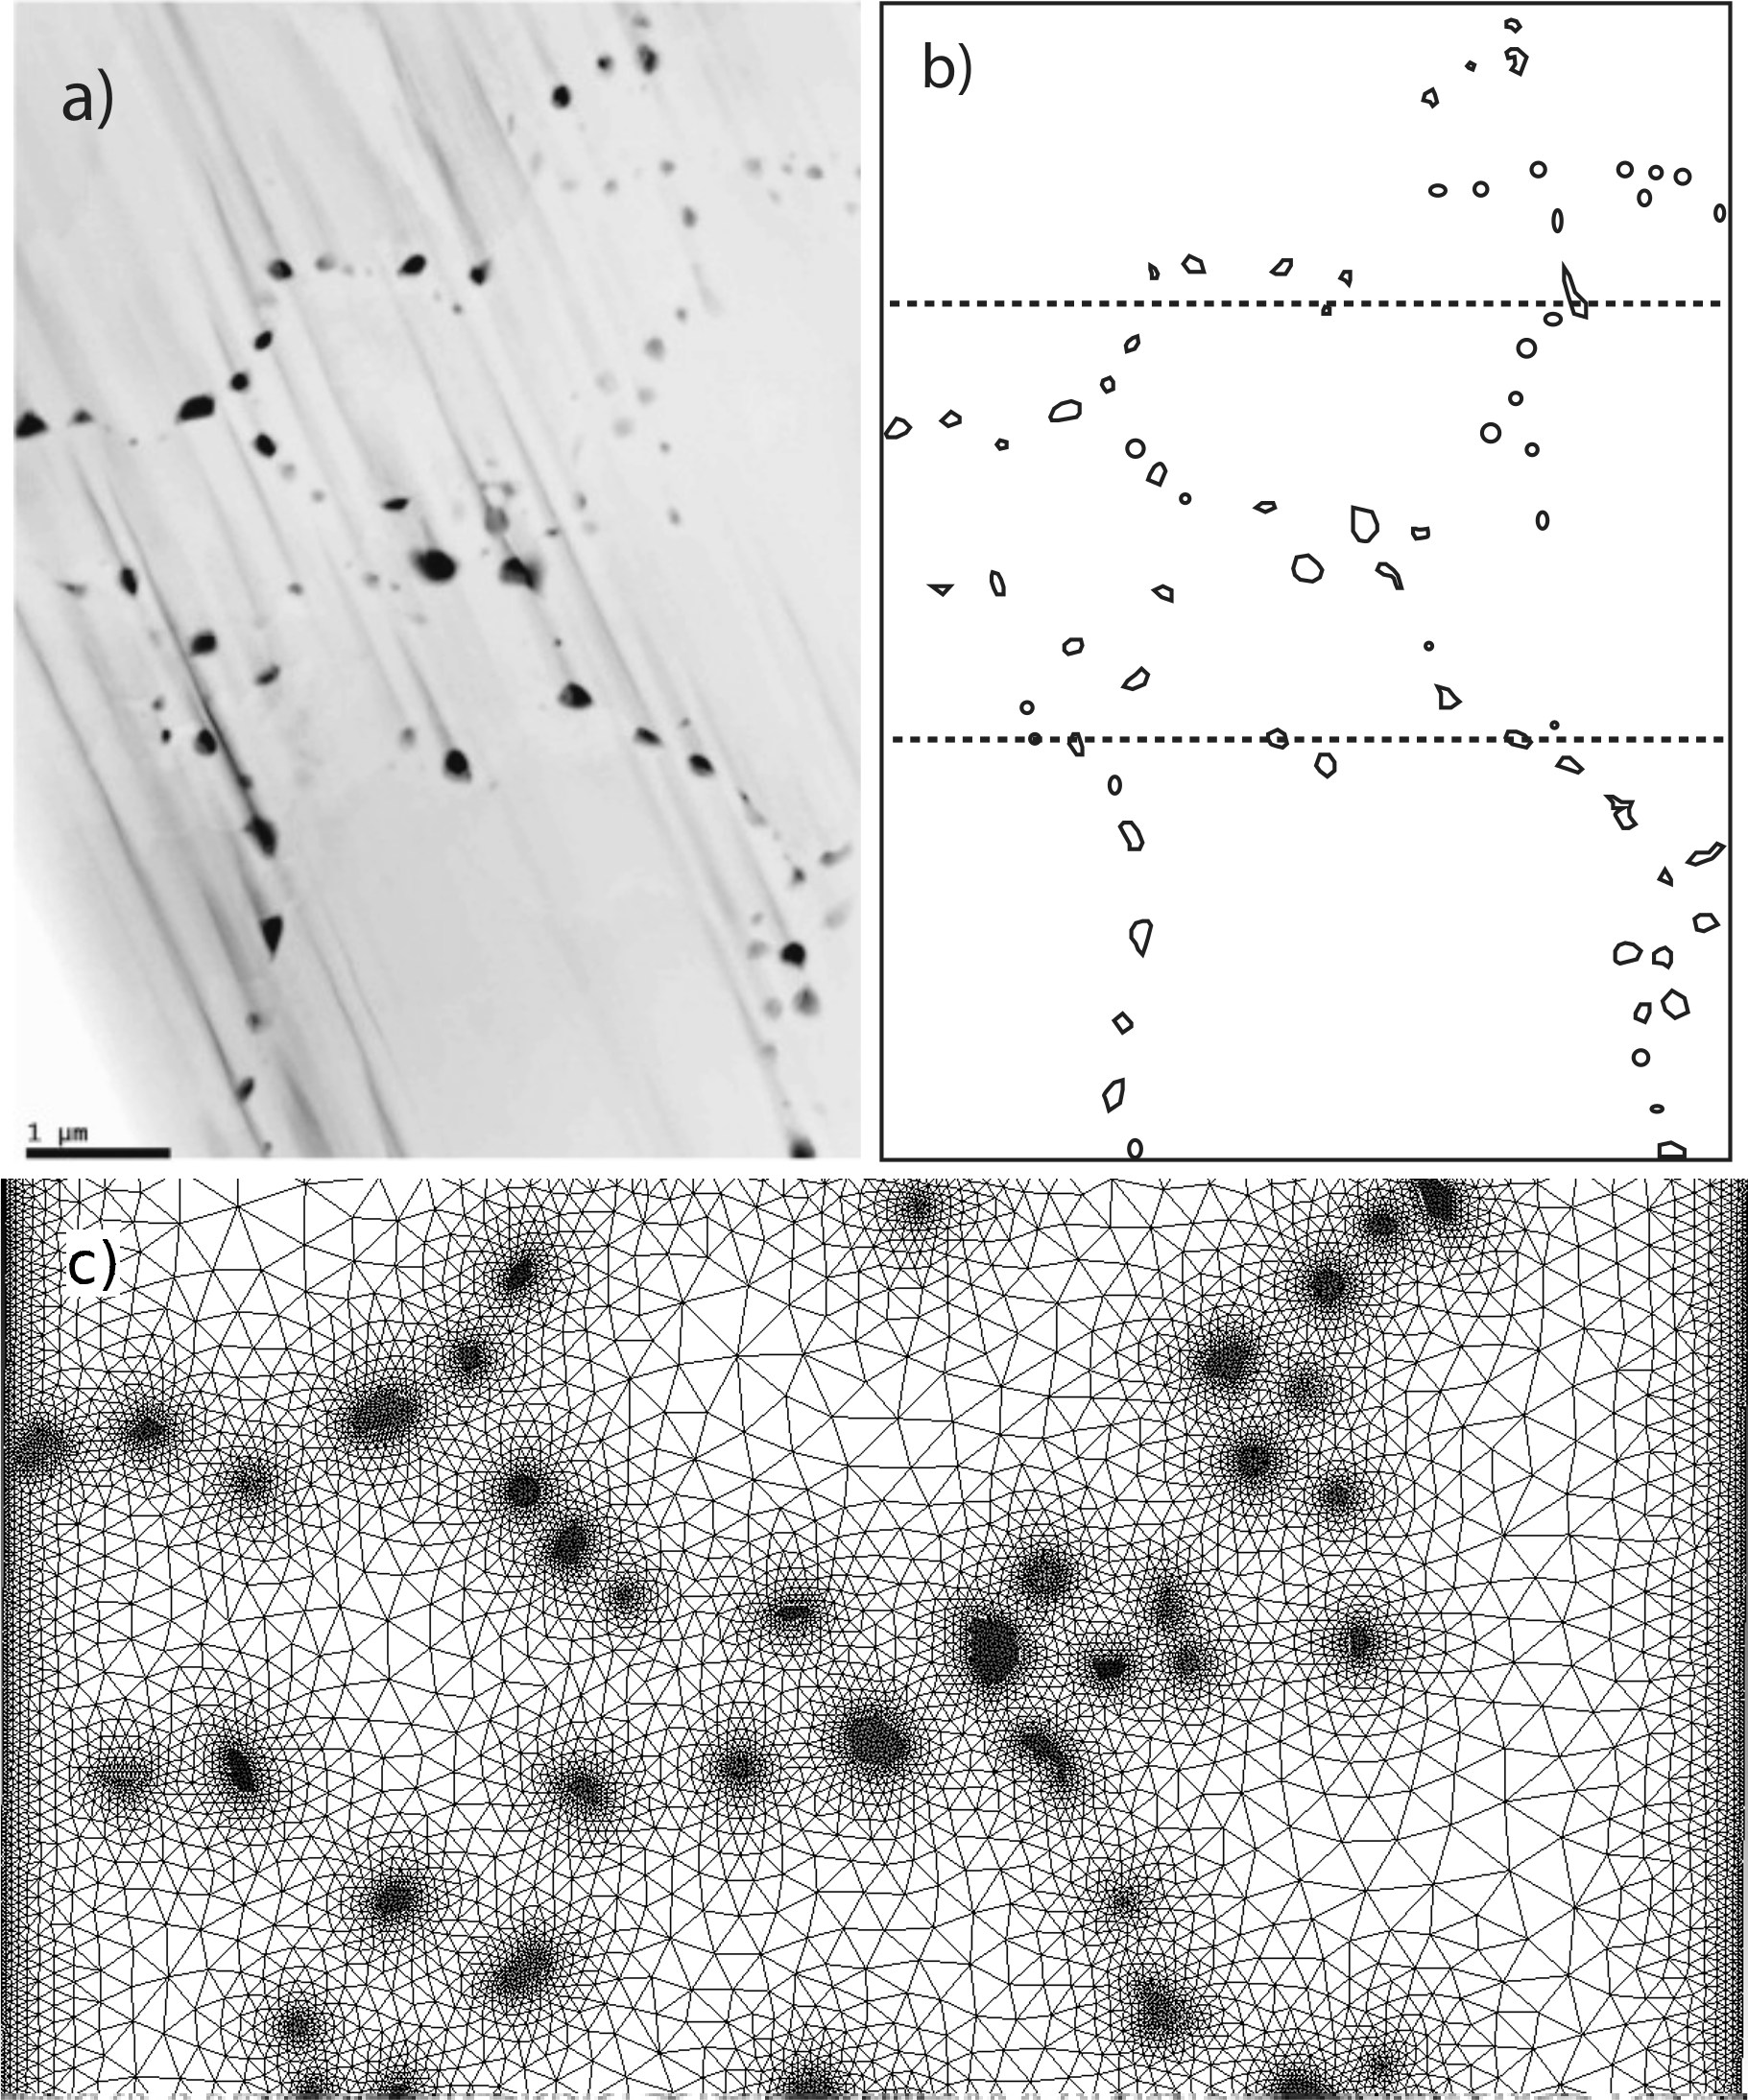
\includegraphics[width=90mm]{grain_boundary_U-10Mo_white_BG}
\caption[(a) SEM image of the fission gas bubbles along the grain boundaries from Miller used for FEM calculations (b) Geometry created based on the grain boundary fission gas image in (a) (c) FEM mesh with grain boundary fission gas of the region between the dotted line in  (b).]{(a) SEM image of the fission gas bubbles along the grain boundaries from Miller \etal~\cite{miller2012advantages} used for FEM calculations (b) Geometry created based on the grain boundary fission gas image in (a) (c) FEM mesh with grain boundary fission gas of the region between the dotted line in  (b). }
\label{fig_Xe_SEM}
\end{figure}
\begin{figure}
\centering
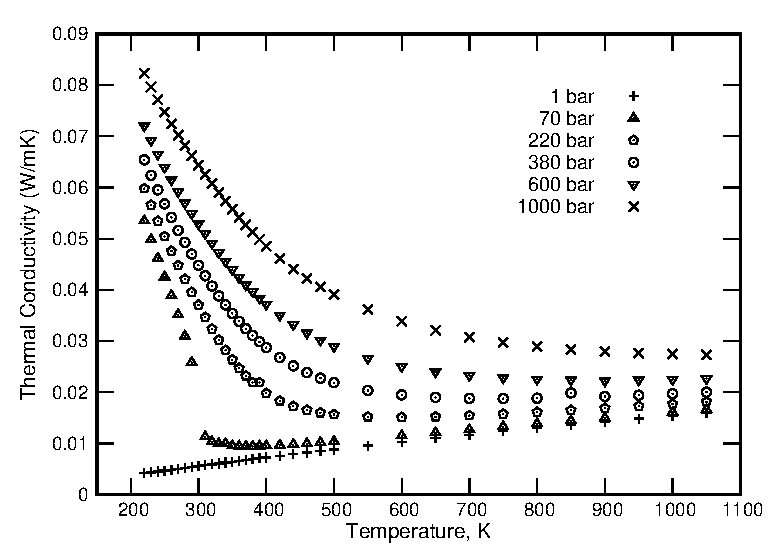
\includegraphics[width=110mm]{Xe_K_eps_rotate}
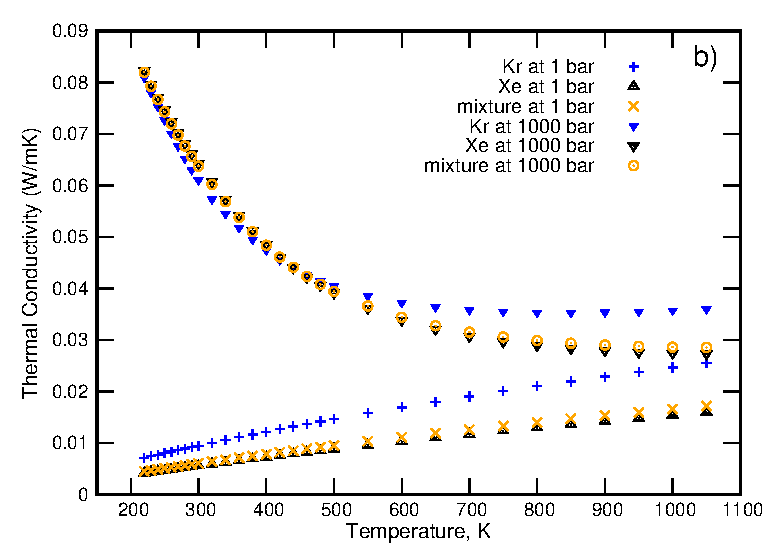
\includegraphics[width=110mm]{krypton_xenon_compare}
\caption[(a) Thermal conductivity of xenon as a function of pressure and
temperature based on the measurements of Rabinovich et
al.]{(a) Thermal conductivity of xenon as a function of pressure and
temperature based on the measurements of Rabinovich et
al.~\cite{rabinovich1987thermophysical}.  Note that the critical point of xenon
is 289.733~K and 58.42~bar; this is why there is such a drastic change in
conductivity at low temperature between the 1~bar and 70~bar isobars.
{(b) Comparison between the thermal conductivities of pure
krypton and pure xenon (both at 1~bar and at 1000~bar) with a mixture of
15\% krypton and 85\% xenon at both 1~bar and 1000~bar. This composition is
representative of fission gas.}}
\label{fig_Xe_pressure}
\end{figure}

The thermal conductivity of \mbox{U-10Mo} was estimated from a linear fit of thermal conductivity as a function of temperature between 298~K and 1073~K from Kaufmann~\cite{kaufmann1962nuclear}. Burkes \etal~\cite{burkes2010thermo} also provided a linear fit of the \mbox{U-10Mo} thermal conductivity as a function of temperature up to 873~K; their results were in good agreement with Kaufmann's~\cite{kaufmann1962nuclear}.
{Xenon conductivity is drawn from the data of Rabinovich \etal~\cite{rabinovich1987thermophysical};}
the thermal conductivity of xenon depends on both temperature and pressure,
as shown in Figure~\ref{fig_Xe_pressure}. The pressure inside a bubble depends on the radius of the bubble, the surface tension, the magnitude of the Burgers vector, and the shear modulus of the host material~\cite{greenwood1959role,trinkaus1983energetics}. According to Xiao \etal~\cite{xiao2015atomistic}, the pressure inside a xenon bubble can be as high as 120~kbar. Such high pressures suggest the possibility of forming solid xenon bubbles inside the fuel~\cite{thomas1991condensed,ross1980condensed,zheng2014thermodynamics}. Unfortunately, thermal conductivity data for xenon above 1000~bar are not available, so we chose two limiting sets of thermal conductivity data: 1~bar and 1000~bar. For each set of data, a polynomial fit (fifth order) was used to interpolate the conductivity over the temperature range.
{Fission gas is typically a mixture of krypton and xenon, so
we ran simulations in which the bubbles were filled with 15\% krypton,
85\% xenon (molar basis), with conductivity data for krypton from Rabinovich \etal~\cite{rabinovich1987thermophysical}. The mixture's thermal conductivity was calculated using Wilke's mixing rule~\cite{wilke1950viscosity}, which uses the full first-order Chapman--Enskog relation along with Eucken's relation for the thermal conductivities~\cite{vincenti1965introduction, alkandry2013comparison}. Using Wilke's approach, the mixture's thermal conductivity is given by
\begin{equation}
  K = \sum_i \frac{x_iK_i}{\sum_j x_j \phi_{ij}},
  \label{eq:K-mixture}
\end{equation}
where $x_i$ is the mole fraction and $K_i$ is the conductivity of the pure
component. The coefficients $\phi_{ij}$ can be calculated by the following
relation~\cite{alkandry2013comparison}:
\begin{equation}
  \phi_{ij} = \frac{\left[1+\left(\dfrac{\mu_i}{\mu_j}\right)^{\!\!1/2}\left(\dfrac{M_j}{M_i}\right)^{\!\!1/4}\right]^2}{\left[
    8\left(1+\dfrac{M_i}{M_j}\right)
  \right]^{1/2}},
\end{equation}
where $M_i$ is the molar mass of the species and $\mu_i$ is the viscosity.
}
\nomenclature{$K$}{thermal conductivity}
\nomenclature{$x_i$}{mole fraction}
\nomenclature{$M_i$}{molar mass}

\subsection{Effective Thermal Conductivity Calculation}
\label{subsec:Keffcalc}
The temperature in a composite material in the absence of heat sources is described by the heat equation:
\begin{equation}
\nabla \cdot \left(K\nabla T \right)=0,
\label{eq:Tdiff}
\end{equation}
where $K(x,y)=\chi_1(x,y)K_1 + \chi_2(x,y)K_2$ is the thermal conductivity tensor, $T$ is the temperature, $K_i\ { }(i=1$ for the matrix and 2 for the bubble) is the thermal conductivity tensor, and $\chi_i(x,y)$ is the indicator function of phase $i$. The local heat flux can be calculated using the equation
\begin{equation}
\label{eq:localflux}
q''(x,y) = -K(x,y) \cdot \nabla T(x,y),
\end{equation}
where $q''(x,y)$ is the local heat flux vector and $\nabla T(x,y)$ is the local temperature gradient. The local temperature and heat flux are calculated by solving Equations~\eqref{eq:Tdiff} and \eqref{eq:localflux}. The components of the effective thermal conductivity tensors are calculated via 
\begin{equation}
\label{eq:Keffcalc}
K_{\text{eff}}^x = -q_x''\left<\frac{\partial x}{\partial T}\right>.
\end{equation}
Where $q''_x$ is the mean heat flux in the $x$-direction, and $\left<\frac{\partial x}{\partial T}\right>$ is the average inverse temperature gradient in the $x$-direction. The MOOSE Framework~\cite{gaston2009moose} was used to solve Equation~\eqref{eq:Tdiff} with Dirichlet boundary conditions at $x=0$ and $x=L$ and Neumann (adiabatic) boundary conditions at $y=0$ and $y=L$. The effective thermal conductivity was calculated using Equation~\eqref{eq:Keffcalc}.



\section{\label{sec:results}Results and Discussion}
%The presence of xenon bubbles which have relatively low thermal conductivity in U-10Mo fuel effectively reduces the heat flow area and thus impacts the rate of overall heat transfer. Xenon bubbles have a broad range of diameters~\cite{miller2015transmission}; the size of the bubbles depends on the fission density and irradiation time. Due to significant size differences between intra- and inter-granular gas bubbles, the calculation of effective thermal conductivity was divided into two steps. In the first step, the thermal conductivity of a single crystal with nanometer-sized intra-granular gas bubbles was calculated. In the second step, the overall thermal conductivity of a polycrystalline material with intra- and inter-granular gas bubbles was calculated. 

\subsection{Effect of Xenon Gas Bubbles on the Thermal Conductivity} 
\label{subsec:xenonbubble}
We examined two broad categories of bubbles: inter-granular bubbles (\ie,
bubbles that collect at grain boundaries) and intra-granular bubbles.
The intra-granular case is intended to represent the effect of a gas bubble
superlattice (GBS) on the conductivity. We will discuss each case in turn.

\subsubsection{Intra-Granular Bubbles}
\begin{figure}%[H]
\centering
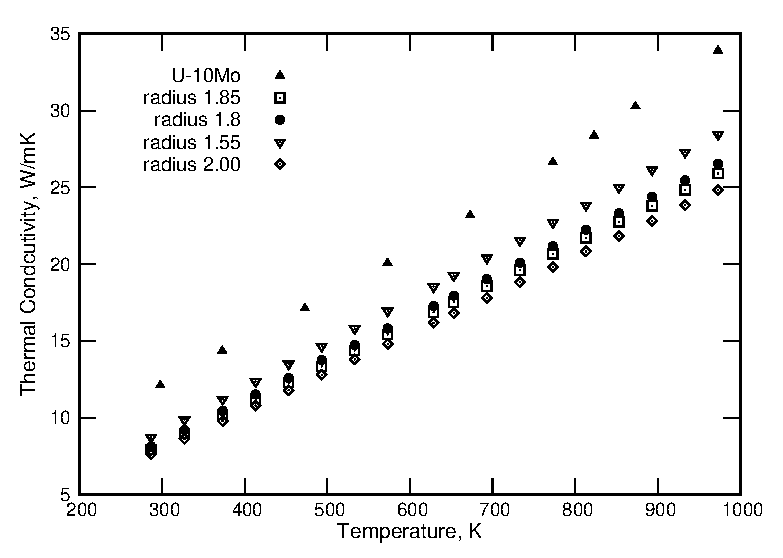
\includegraphics[width=110mm]{result_eps_rotate_bold}
\caption[Comparison between the thermal conductivity of \mbox{U-10Mo}
  (from Kaufmann) to the effective thermal
  conductivity of \mbox{U-10Mo} with intra-granular xenon bubbles of different
  diameters as arranged in Figure~\ref{gbs}b.]{Comparison between the thermal conductivity of \mbox{U-10Mo}
  (from Kaufmann~\cite{kaufmann1962nuclear}) to the effective thermal
  conductivity of \mbox{U-10Mo} with intra-granular xenon bubbles of different
  diameters as arranged in Figure~\ref{gbs}b.}
\label{fig_result_intra}
\end{figure}

A two-dimensional representation of a gas bubble superlattice, as shown in
Figure~\ref{gbs}, was used to simulate the effect of intra-granular bubbles on the thermal conductivity.
Five different bubble sizes were used, each with the same superlattice
constant (resulting in the same center--center distance between bubbles).
Figure~\ref{fig_result_intra} shows the effective thermal conductivity due to the xenon bubble distribution in the intra-granular region.
As is clear from Figure~\ref{fig_result_intra}, the thermal conductivity decreases with increasing bubble size, and is 20--40~percent lower in all cases than it is for bubble-free U-10Mo. In these simulations, the thermal conductivity of xenon was assumed constant at its 1~bar value (it is still a function of temperature).
Figure~\ref{fig_compare} shows the result of the finite element method solution compared with the theoretical solution for porous materials' thermal conductivity from the Maxwell--Eucken equation~\cite{maxwell1881treatise}, 
\begin{equation}
	\lambda = \lambda_s\frac{\lambda_p+2\lambda_s+2\nu_p(\lambda_p-\lambda_s)}{\lambda_p+2\lambda_s-\nu_p(\lambda_p-\lambda_s)},
	\label{eq_MaxEuck}
\end{equation}
where $\lambda$ is the effective thermal conductivity of the fuel, $\lambda_s$ is the thermal conductivity of the continuous phase (U-10Mo), $\lambda_p$ is the thermal conductivity of the dispersed phase (xenon bubble), $\nu_p$ is the volume fraction of the dispersed phase (\ie., the volume fraction of xenon in U-10Mo). Equation~\eqref{eq_MaxEuck} assumes the pore volume fraction is less than 15~percent, that the pores are dispersed uniformly in the solid, and that the distance between the pores is large enough that they do not interact~\cite{clark2003monolithic,smith2013thermal}. The result is also compared with the Hashin--Shtrikman upper bound, which is based on a theoretical expression derived for the magnetic permeability of a multiphase material~\cite{hashin1962variational},
\nomenclature{$\lambda$}{the effective thermal conductivity of the fuel}
\begin{equation}
\lambda = \frac{1}{4}\biggl[ \lambda_p(3\nu_p-1) + \lambda_s(2-3\nu_p)+ \Bigl( \left[ \lambda_p (3\nu_p -1) + \lambda_s(2-3\nu_p) \right]^2 + 8\lambda_s\lambda_p \Bigr)^{\frac{1}{2}}
    \biggr].
\label{eq:Hash-Sht}
\end{equation}

\begin{figure}%[t]
	\centering
	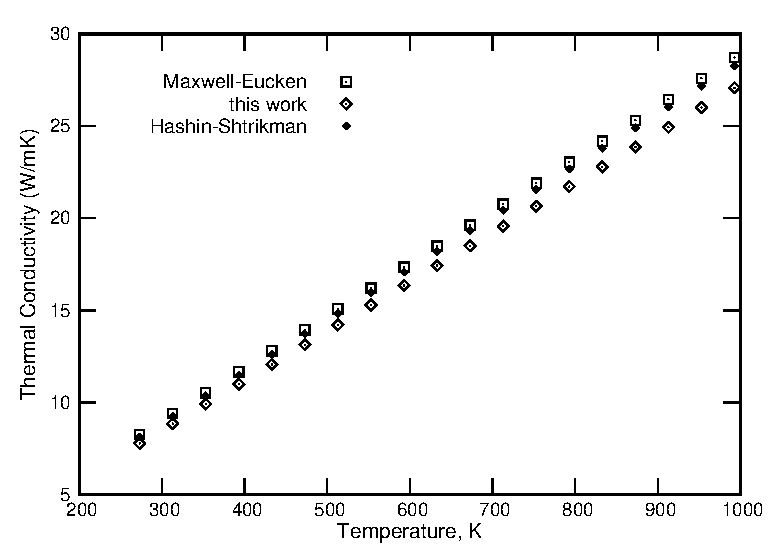
\includegraphics[width=110mm]{theory_compare_eps_rotate_bold}
	\caption[Comparison of the calculated effective thermal conductivity of \mbox{U-10Mo} with intra-granular xenon bubble (radius 1.55~nm, 10$\%$ porosity) with the Maxwell--Eucken and Hashin--Shtrikman models]{Comparison of the calculated effective thermal conductivity of \mbox{U-10Mo} with intra-granular xenon bubble (radius 1.55~nm, 10$\%$ porosity) with the Maxwell--Eucken~\cite{maxwell1881treatise} and Hashin--Shtrikman~\cite{hashin1962variational} models. In all cases, we find that the
      two theoretical models over-predict the thermal conductivity by about
      5--10~percent compared with the numerical solution.}
	\label{fig_compare}
\end{figure}

%The Hashin--Shtrikman limit agrees well with our results.
Figure~\ref{fig_compare} shows the effect of distributed gas bubbles in the intra-granular region (grain boundary bubbles were not included). Both theoretical models over-predict the conductivity by 5--10~percent, and the absolute error increases with temperature.

\subsubsection{Inter-Granular Bubbles}
Inter-granular fission gas bubbles are associated with bubbles that collect on
or near grain boundaries. Bubbles are naturally drawn to grain boundaries
because of the excess volume that accompanies grain boundaries, as well as
the decreased energy associated with void formation at grain boundaries
relative to the bulk.

To evaluate the effect of inter-granular fission gas on the overall thermal conductivity, Figure~\ref{fig_Xe_SEM}b was used as the simulation domain. As can be seen in Figure~\ref{fig_Xe_SEM}, fission gas bubbles trapped on grain boundaries do not have consistent shapes. Note that this is only a snapshot in time of the grain structure: as burnup increases, the stress in the fuel changes, more fission gas is evolved, and the grains can rotate and change shape. For simplicity, the thermal conductivity values at 1 bar were used for xenon. 
It should be noted that this only includes the effect of the bubbles gathered
at the grain boundary: effects on the conductivity associated with the grain
boundaries themselves, which will result in changes in the conductivity
because of phonon scattering effects (which are a minor contribution to thermal
conductivity in metals), as well as any effects associated with U--Mo
segregation at the grain boundary, are neglected in this model.

%Xenon's thermal conductivity was kept constant at its 1~bar value (though it is still a function of temperature).
The presence of these (intra- and inter-granular) xenon bubbles decreased the thermal conductivity by more than 25~percent, as shown in Figure~\ref{fig_eff_K_GB}. According to Miller \etal~\cite{miller2012advantages},
their sample (on which our simulations are based) went through a fission density of $3.46\times10^{21}$~fission/cm$^{3}$. At this fission density, Burkes and coworkers~\cite{burkes2015thermal} found that the experimental thermal conductivity of \mbox{U-10Mo} reduced to almost 33~percent of its unirradiated value at 473~K\@. It should
be noted that the real material has a three-dimensional grain boundary structure with varying levels of fission gas at each cross section, meaning our estimates of the thermal conductivity (which effectively assume rod-like inclusions rather than spheres) will be too low. Past
studies~\cite{bakker1997using,Schulz1981} have indicated that
conductivity in the presence of inclusions is underestimated in two-dimensional
models. This suggests that the measured conductivity (33\% of the
conductivity of the unirradiated material) may be reasonably consistent with the conductivity estimated here (\ie, 25\% of the conductivity of the unirradiated material).

\begin{figure}
	\centering
	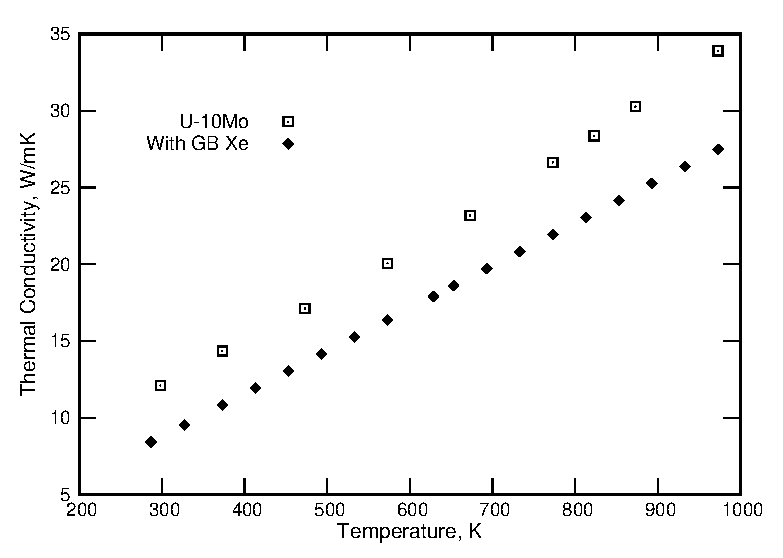
\includegraphics[width=110mm]{result_Xe_GB_eps_rot_bold}
    \caption[Comparison between the thermal conductivity of bubble-free
      \mbox{U-10Mo} with that of \mbox{U-10Mo} that has xenon bubbles
      decorating the grain boundaries according to the distribution in
      Figure~\ref{fig_Xe_SEM}]{Comparison between the thermal conductivity of bubble-free
      \mbox{U-10Mo} with that of \mbox{U-10Mo} that has xenon bubbles
      decorating the grain boundaries according to the distribution in
      Figure~\ref{fig_Xe_SEM}. A 4\% drop is observed, increasing with
      temperature.}
	\label{fig_eff_K_GB}
\end{figure}

\subsection{Effect of Xenon Pressure on the Overall Thermal Conductivity}
\label{subsec:xenonpressure}
To evaluate the impact of the pressure of the xenon bubbles on the overall thermal conductivity, we performed a study of the overall conductivity as a function of temperature for five different xenon bubble pressures given a fixed bubble distribution (Figure~\ref{gbs}b). Each pressure has a distinct thermal conductivity (Figure~\ref{fig_Xe_pressure}) as a function of temperature. In this part of the study, a constant bubble size was used (radius 1.55~nm). The results are shown in Figure~\ref{fig_press_K}. The results show little to no change of the overall thermal conductivity of the fuel due to the bubbles' pressure over the range studied. However, though xenon has a wide range of thermal conductivities at different pressures (see Figure~\ref{fig_Xe_pressure}), the effect is negligible relative to the thermal conductivity of the fuel. 

Also shown in Figure~\ref{fig_press_K} is the overall conductivity of the
system in Figure~\ref{gbs}b for bubbles filled with an 85\% xenon, 15\%
krypton mixture, with the mixture's conductivity given by
Equation~\eqref{eq:K-mixture}, using pure-component conductivities at both
1~bar and 1000~bar.  The overall conductivity is nearly identical
in all cases, indicating that the overall conductivity is not a strong
function of pressure or composition under these conditions.

\begin{figure}
	\centering
%scale=.43
	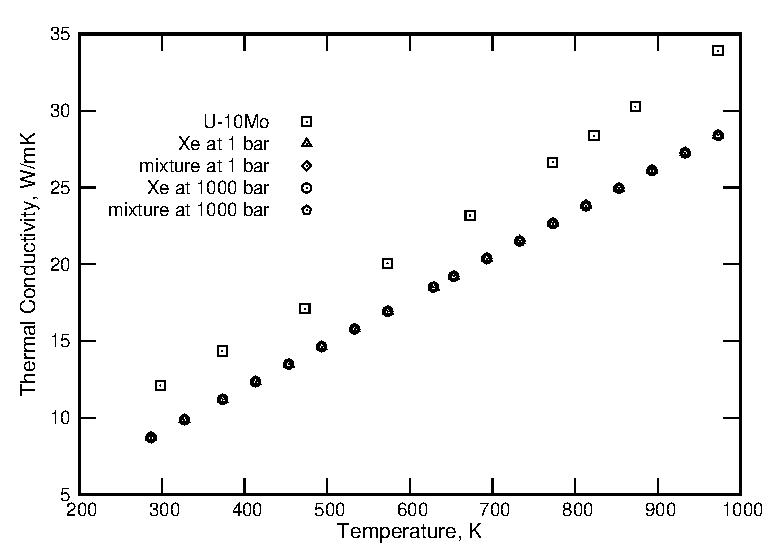
\includegraphics[width=100mm]{press_eff_k_rotate_bold}
	\caption[Overall thermal conductivity of \mbox{U-10Mo} using the thermal 
        conductivity of xenon at two extremes of pressure
        (1~bar and 1000~bar), compared to that of pure (bubble-free) \mbox{U-10Mo}]{Overall thermal conductivity of \mbox{U-10Mo} using the thermal 
        conductivity of xenon at two extremes of pressure
        (1~bar and 1000~bar), compared to that of pure (bubble-free) \mbox{U-10Mo}.
        Bubbles are distributed as in Figure~\ref{gbs}b with radii of 1.55~nm.
        {Also shown for reference is the effective thermal
        conductivity that would result from the same bubbles filled with a
        15~atom\% krypton, 85~atom\% xenon mixture (representative of fission
        gas) at both 1~bar and 1000~bar.}}
	\label{fig_press_K}
\end{figure}
%Based on our results, xenon bubbles reduces the thermal conductivity more than 25$\%$. The experimental thermal conductivity reduces much more. This is due to several factors. Fission bubbles have a wide range of sizes and shapes. Also thermal conductivity of U-Mo system is sensitive to the Mo concentration. It decreases with the increase of molybdenum concentration~\cite{kaufmann1962nuclear, burkes2015thermal}. Because molybdenum is a fission product, it further enhances. There is a diffusion barrier between the Aluminum cladding and fuel, which is usually Zr. These two layers create the contact resistance, that would affect the heat flow.

\subsection{Effect of Bubble Arrangement on Thermal Conductivity}
\label{subsec:area}
We performed a series of simulations to determine whether bubble distribution has a significant influence on the overall thermal conductivity. Two cases were considered. In the first case, we used same number (16) of bubbles of the same diameter (1 nm) and organized them into five different arrangements. The arrangements are arbitrary, but each has the same area fraction of bubbles (xenon gas). In the first arrangement (Figure~\ref{fig:five_figures}a), the bubbles are dispersed uniformly throughout the domain. In Figure~\ref{fig:five_figures}b, the bubbles are arranged in a denser pattern with bubble-free portions near the high-temperature side. In Figure~\ref{fig:five_figures}c, the bubbles are arranged in one corner. In Figure~\ref{fig:five_figures}d, the bubbles are tightly clustered near the center of the domain, creating significant bubble-free regions at the top and bottom. The overall thermal conductivities for these arrangements are presented in Figure~\ref{fig:five_results}.
In these simulations, heat is flowing from left to right, whereas the top and bottom boundaries are insulating (adiabatic).

Based on the results from Figure~\ref{fig:five_figures}, arrangement (d) shows a minor deviation, particularly at high temperatures, compared to the other arrangements. The other four bubble arrangements do not produce significantly different thermal conductivities. The reason for the deviation for case~(d) is the relatively wide ``heat channel'' in the direction of the heat flow, which is absent in the other arrangements. The highest thermal conductivity difference between Figure~\ref{fig:five_figures}d and the other arrangements is approximately 0.93~W/m$\cdot$K, which is also a function of the open channel's area.

\begin{figure}
	\centering
	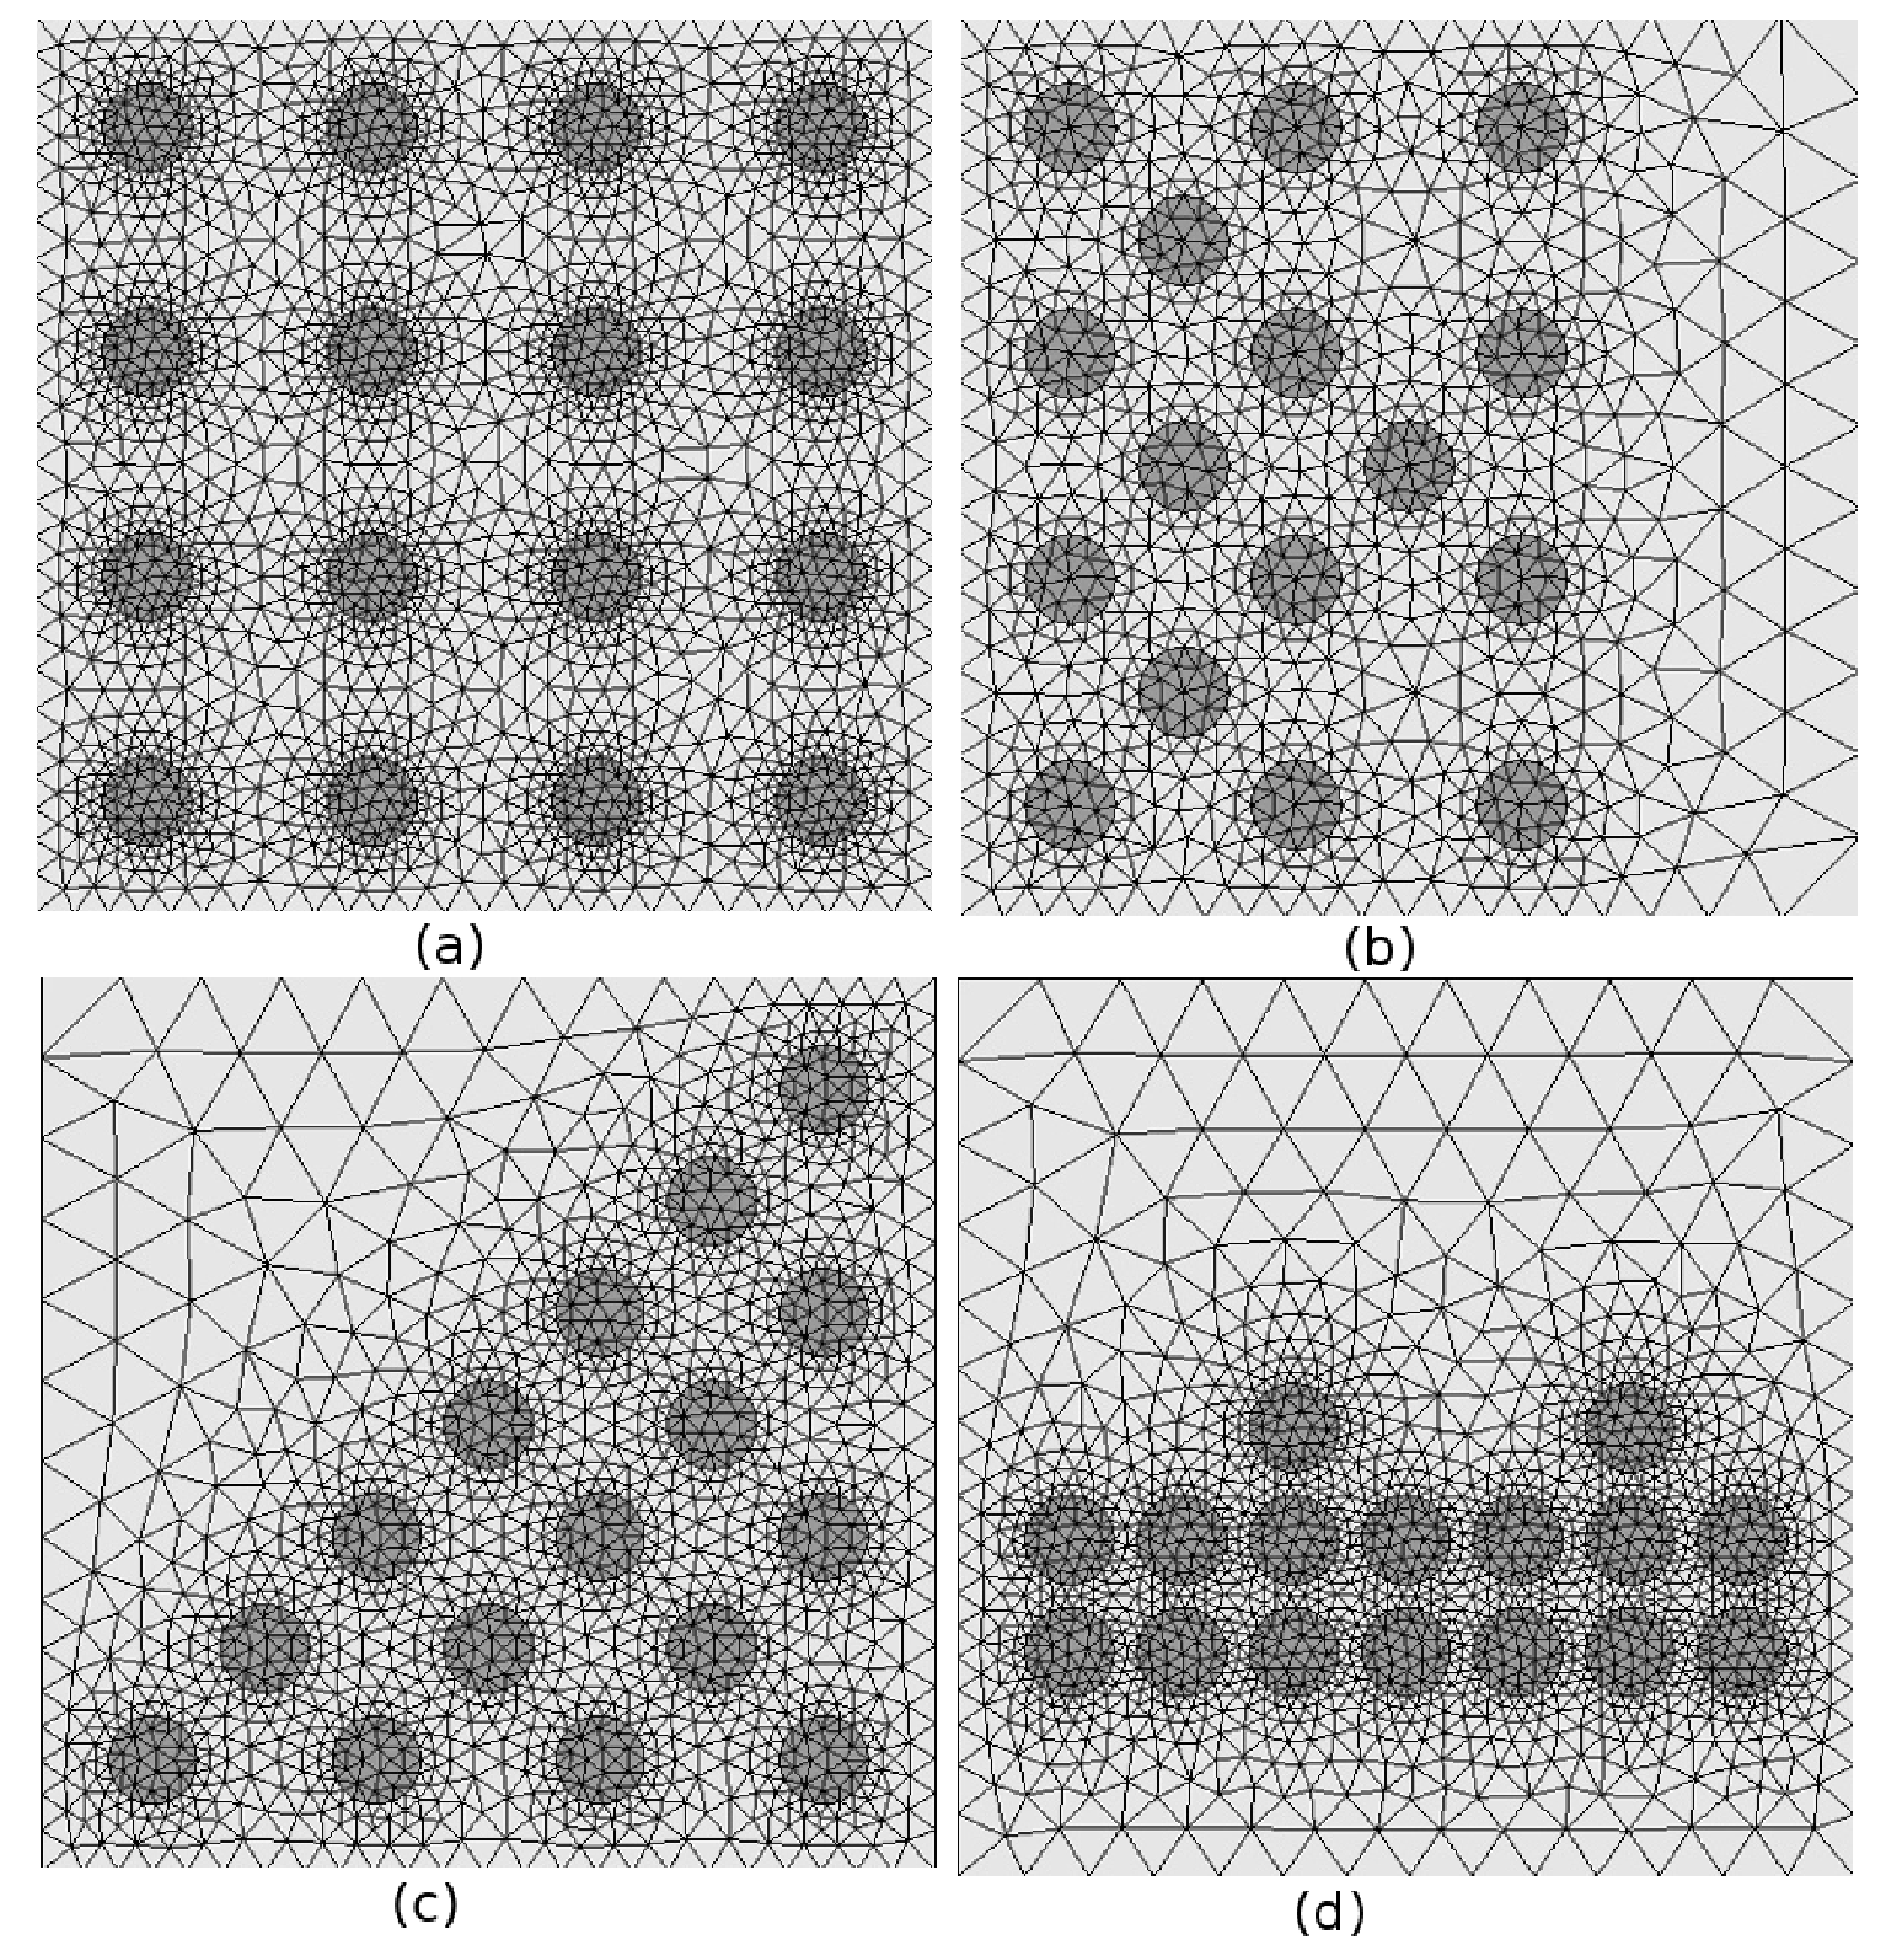
\includegraphics[width=110mm]{2x2_abcd_gray}
    \caption[Different bubble arrangements in which the area of each bubble and
      the number of bubbles are the same]{Different bubble arrangements in which the area of each bubble and
      the number of bubbles are the same. Heat flows from left to right in
      these simulations; only arrangement (d), with its uninterrupted ``heat
      channel'' in the top half of the domain, shows significantly different
      conductivity.}
	\label{fig:five_figures} 
\end{figure}

\begin{figure}
	\centering
	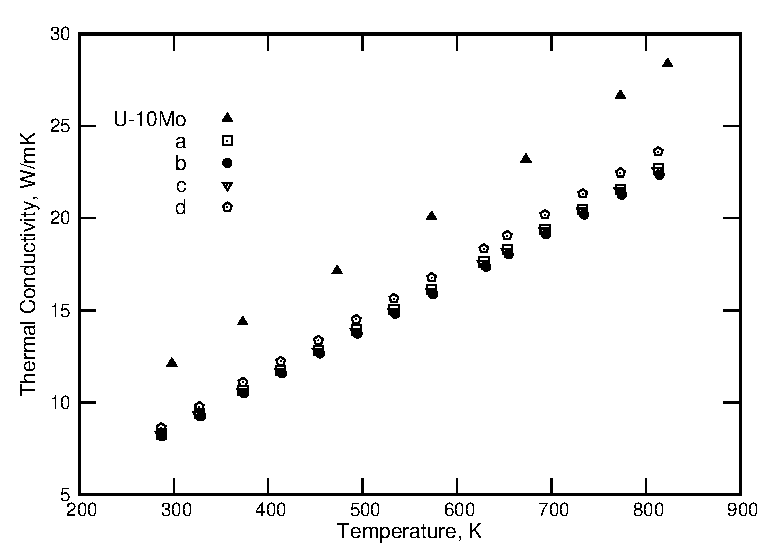
\includegraphics[width=110mm]{result_area_compare_eps_bold_rotate}
    \caption[Comparison of the calculated thermal conductivity of different
        bubble arrangements (constant bubble area and diameter corresponding to Fig.~\ref{fig:five_figures}). ]{Comparison of the calculated thermal conductivity of different
        bubble arrangements (constant bubble area and diameter corresponding to Fig.~\ref{fig:five_figures}). Only
        arrangement (d), with its properly-oriented ``heat channel,'' shows significant
        differences from the others, and such differences are relatively
        insignificant compared to the bubble-free conductivity.}
	\label{fig:five_results}
\end{figure}

In the second case, different bubble sizes were used with constant total area. As the first case shows, bubble arrangement has minimal impact on the overall heat transfer unless it produces a significant heat transfer channel in direction of the heat flow. In this step, we kept the total area covered by the bubbles the same, but with different sizes of bubbles. To keep the area same while decreasing the bubble diameter, the number of bubbles increases. Figure~\ref{fig:area_same_four} shows the four different arrangements with different bubble sizes. None of the arrangements creates a heat transfer channel in the direction of heat flow. The results are shown in Figure~\ref{fig:four_results}. The results show no significant change in the overall thermal conductivity. We conclude that the bubble arrangement has little impact unless it produces a significant bubble-free heat transfer channel. 

 
\begin{figure}
	\centering
	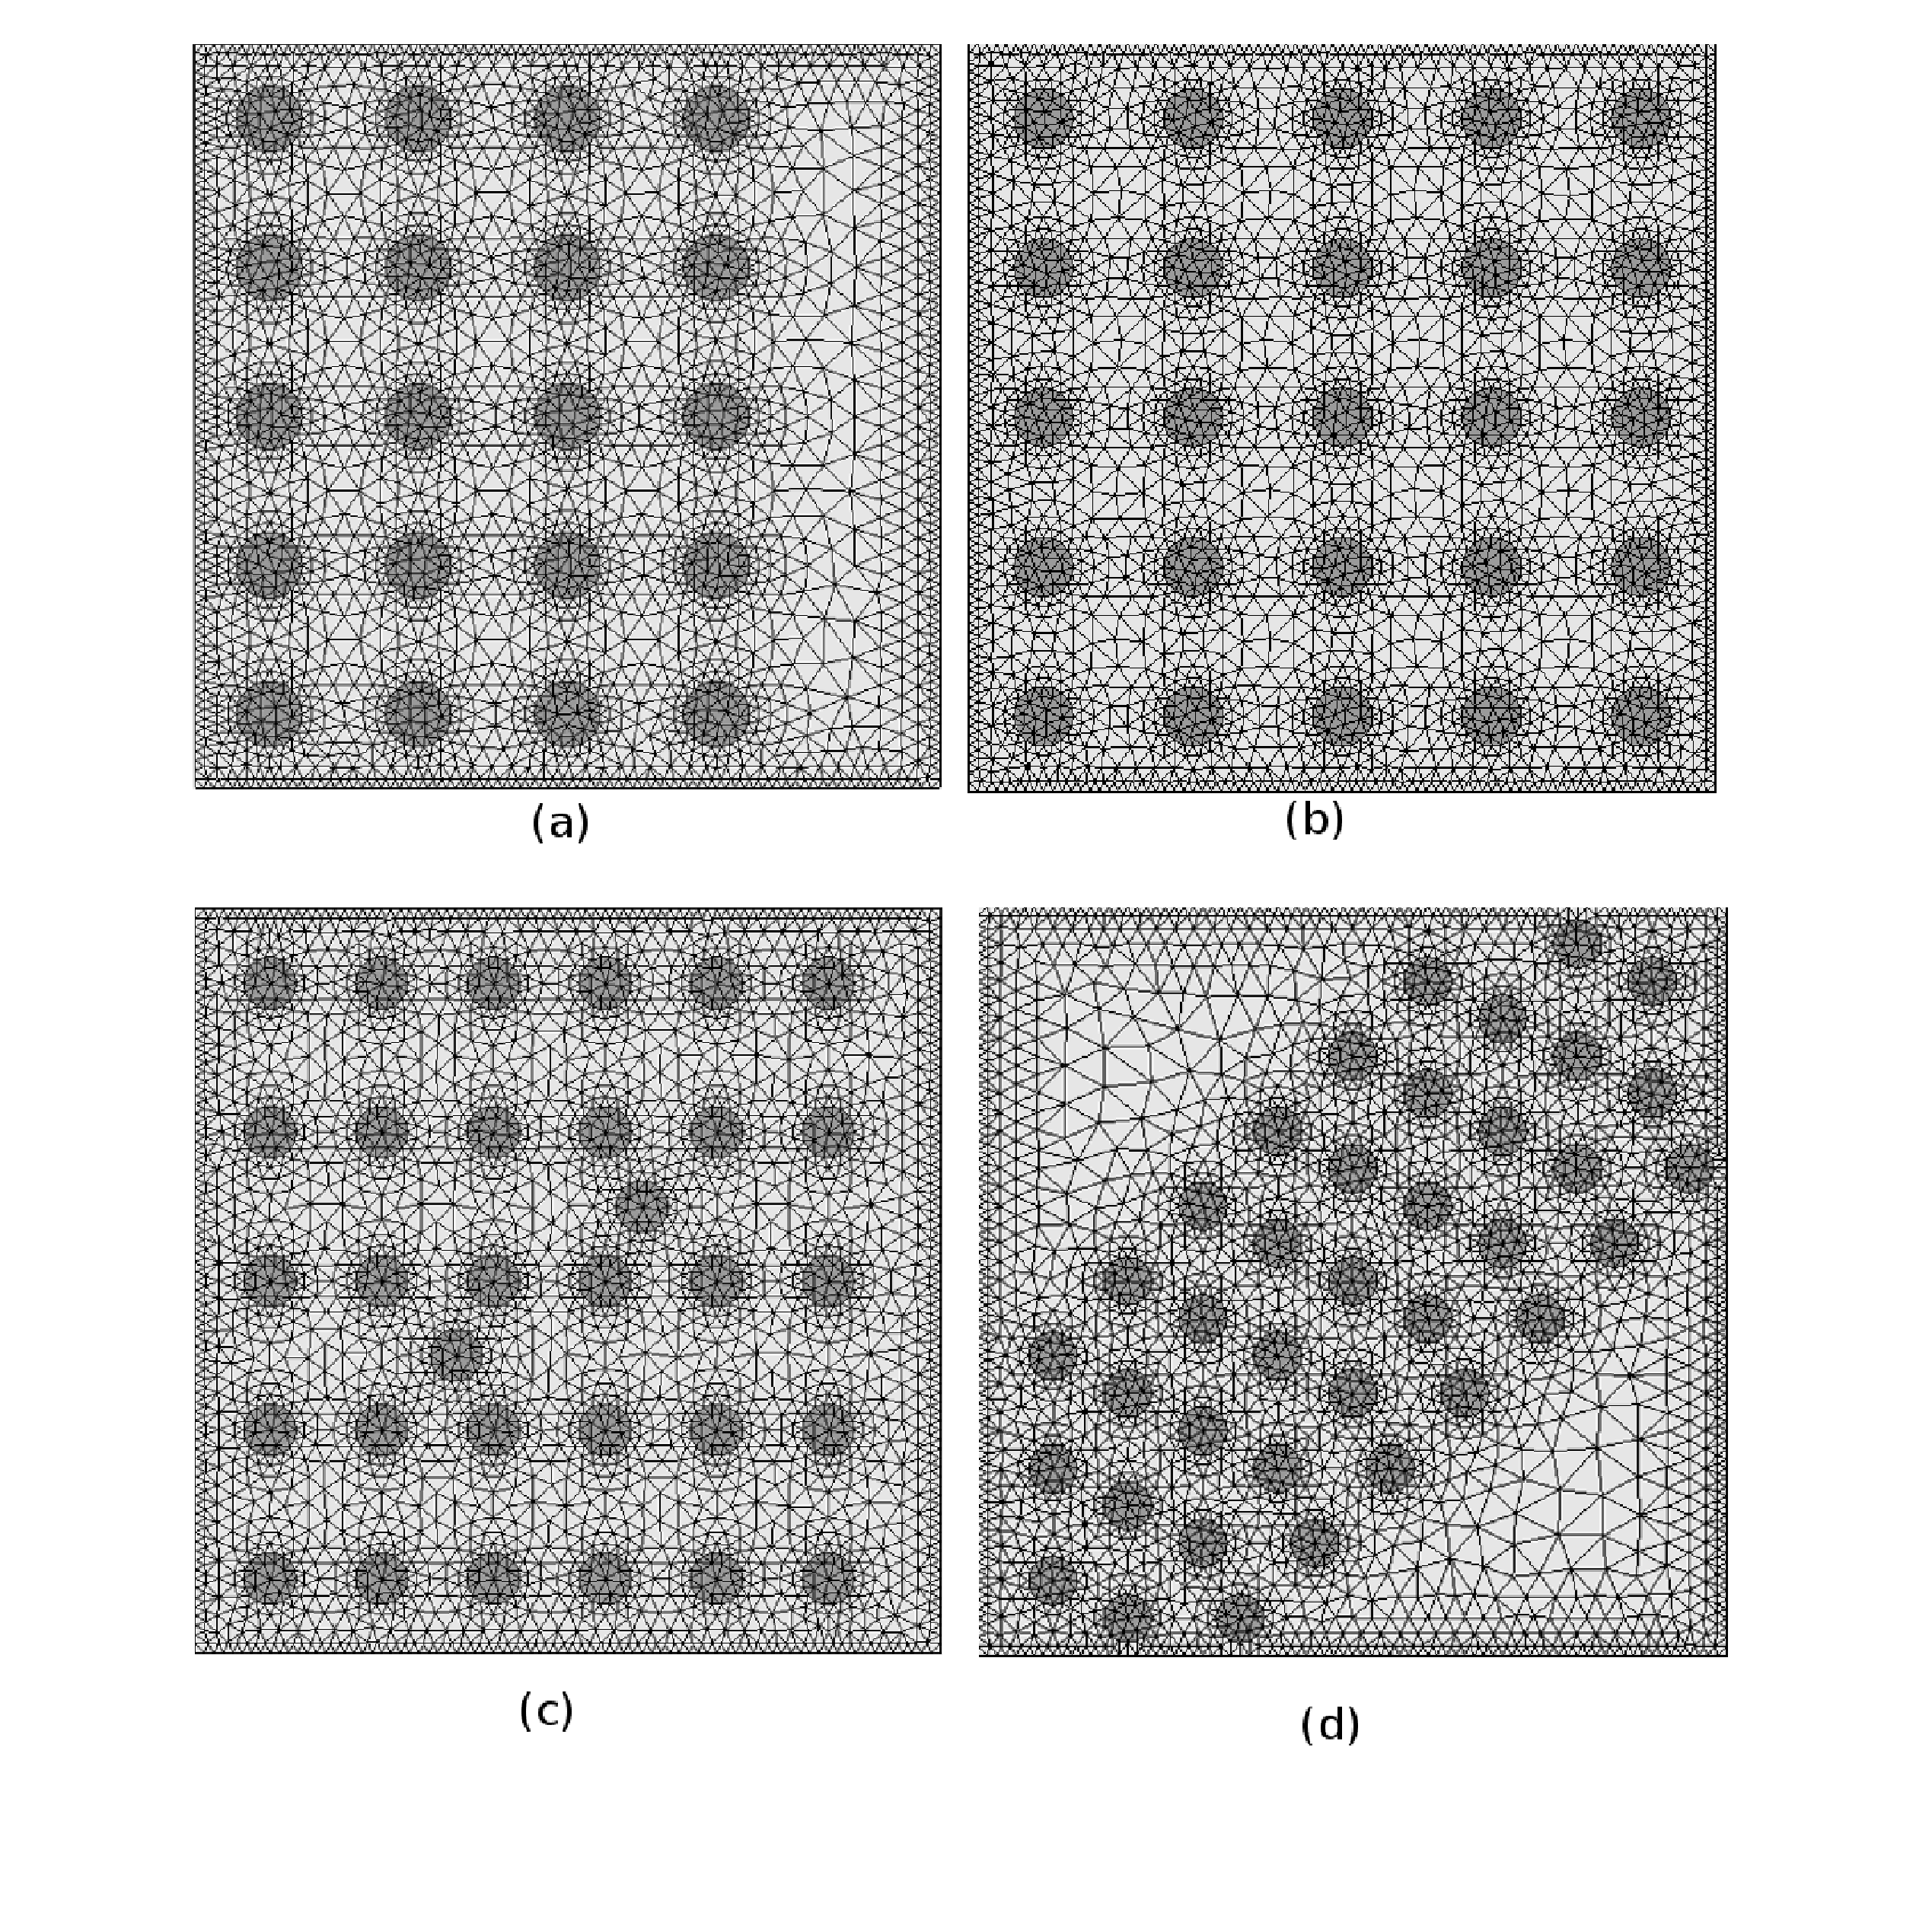
\includegraphics[width=110mm]{same_area_four_figure_gray}
    \caption{Different bubble arrangements where the area is the same but the
      bubbles have different diameters. (a)~20 bubbles, (b)~25 bubbles,
      (c)~32 bubbles, (d)~38 bubbles.}
	\label{fig:area_same_four}
\end{figure}
\begin{figure}
	\centering
	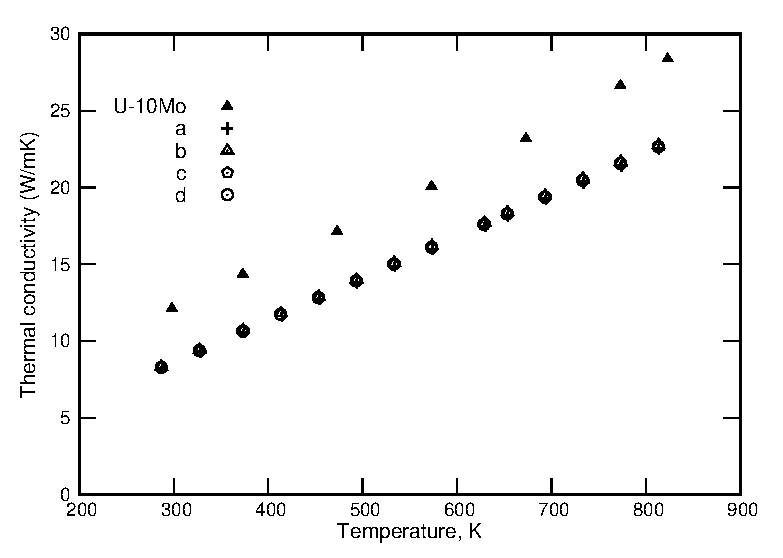
\includegraphics[width=110mm]{area_same_result}
	\caption[Comparison of thermal conductivity between different bubble 
      diameters at constant total bubble area with bubble-free U-10Mo. Bubble
      arrangements are shown in Figure~\ref{fig:area_same_four}]{Comparison of thermal conductivity between different bubble 
      diameters at constant total bubble area with bubble-free U-10Mo. Bubble
      arrangements are shown in Figure~\ref{fig:area_same_four}.
      Bubble diameters are (a) 0.894 nm (b) 0.8 nm (c) 0.707 nm and (d) 0.6488 nm;
      the bubble area fraction is 12.6$\%$~percent.}
	\label{fig:four_results}
\end{figure}

%this is the new addition on the discussion
In our calculation, grain boundary xenon gas bubbles had very minimal impact on the overall heat transfer. That is because our sample has very low grain boundary fission gas areal density, less than 2$\%$ of the total area. Grain boundary fission gas bubble size increases with an increase in burnup~\cite{kim2011fission}.
With an increase in fission density, more fission gas usually diffuses to the grain boundary area and recrystallization~\cite{kim2013recrystallization} subdivides the grains to accommodate the fission gas near the grain boundaries.
This also increases the grain boundary fission gas density. Our results were also compared with porosity correction models, specifically those of Bauer~\cite{bauer1995pile} and Peddicord~\cite{peddicord1978porosity}. Bauer's model ($\lambda=\lambda_0 e^{-2.14\nu}$, where $\lambda_0$ is the thermal conductivity of the 100\% dense material and $\nu$ is the porosity) over-predicts the porosity correction factor for thermal conductivity. Peddicord's model ($\lambda=\lambda_0(1-\nu)^{2.58}$) agrees better with the effective thermal conductivity from our simulations. All these empirical models are applicable to intragranular gas bubbles with uniform distribution and negligible fission gas thermal conductivity.
In our calculation, all the thermal conductivities are measured from two-dimensional finite element models, but two-dimensional thermal conductivity usually represents the lower limit of the three-dimensional thermal conductivity~\cite{bakker1995determination}. Accurate estimation of this limit is very important. 

\section{\label{sec:conclusion}Conclusions}
Estimating the thermal conductivity of nuclear fuel is an important part of understanding fuel behavior in nuclear reactors. In our work, xenon gas was used to represent fission gas bubbles in \mbox{U-10Mo} monolithic fuels. The impact of distributed xenon bubbles on the overall thermal conductivity of \mbox{U-10Mo} is significant, resulting in a 25--35~percent drop in conductivity for the bubble volume fractions studied, largely independent of bubble arrangement. Both intra- and inter-granular gas bubble structures were used. For intra-granular bubbles, a gas bubble superlattice structure was used. The results indicate that the Maxwell--Eucken and Hashin--Shtrikman models overestimate thermal conductivities by at least 5\% for the bubble volume fractions studied.

The pressure dependence of xenon's thermal conductivity was also studied to estimate the impact of bubble pressure on the overall thermal conductivity of \mbox{U-10Mo}. Our results indicate that bubble pressure is not a significant factor for the bubble densities studied---the overall thermal conductivity remains largely unchanged between 1~bar and 1000~bar.
We also find that there is little difference between pure xenon bubbles and
85\% xenon--15\% krypton bubbles from the perspective of overall thermal
conductivity in bubble-laden \mbox{U-10Mo}.

We find that both intra- and inter-granular xenon bubbles reduce the overall thermal conductivity by more than 25~percent. Different bubble arrangements have very little impact on the overall heat flow, unless the arrangement leads to a significant bubble-free channel through which heat can be conducted without interference from nearby bubbles. Bubble size is also not a significant factor, as different bubble sizes at the same bubble areal density produce a U-10Mo slabs with identical overall conductivity.

{We did not consider the effects of solid
fission products and their influence on the overall thermal conductivity. We
believe that this issue needs a complete and thorough investigation, because the
chemical state and the distribution of the solid fission products of U--Mo may
make important contributions to the overall conductivity.}
Future work should also study, quantitatively, the contact resistance between
the cladding and fuel, as well as the evolution of grain boundaries with time
and the influence of local molybdenum concentration on thermal conductivity.




%\bibliographystyle{iopart-num}
\bibliographystyle{apsrev4-2}
\bibliography{abbreviated,final}
%\bibliography{abbreviated,xnthrm}


\chapter{Pseudopotential for Plane-Wave Density Functional Theory Studies of Metallic Uranium}
\textit{This chapter was largely published as an article in \textup{Computational Materials \mbox{Science}}. The authors of that article are A. Rafi M. Iasir and Karl D. Hammond of the University of Missouri.}

\section{Introduction}\label{sec_intro}
Uranium is the heaviest naturally-occurring element on Earth. The discovery of
fission in uranium (specifically, in $^{235}$U) impacted not only scientists
and engineers all over the world, it also changed global politics forever. In
nuclear research, the nucleus of the uranium atom is of much more importance
than the electrons surrounding it, but the electronic structure is important
to the thermodynamic properties, including crystal structure. The structural
features are particularly important to the study of next-generation nuclear
fuels, such as \text{U--10Mo}, that are based on metallic uranium.
The electronic behavior of uranium, along with other light actinides (Pa--Pu),
results in a low-symmetry crystal structure at ambient temperature and
pressure---most metallic elements take on relatively high-symmetry structures
(bcc, fcc, and hcp), but the light actinides are either orthorhombic or
monoclinic at standard temperature and pressure~\cite{Soderlind1995}.
Pure uranium exists in three different solid phases at atmospheric pressure,
depending on the temperature:
\textalpha\ (base-centered orthorhombic), \textbeta\ (tetragonal) and
\textgamma\ (body-centered cubic). At atmospheric pressure, \textalpha-uranium
transforms to \textbeta-uranium at approximately 935~K, and \textbeta-uranium transforms to
\textgamma-uranium at approximately
1045~K~\cite{lawson1988structure,akella1997structural}.
The influence of $5f$
electron--electron correlation plays a pivotal role in the crystallographic
behavior of uranium and other light
actinides~\cite{lander2003gh,freemanHandbook1984}; with this in mind, proper
representation of uranium's $5f$ electrons is very important.

The stability of the crystal structures of the inner transition metals has been
the target of several electronic structure studies.
Eriksson and coworkers~\cite{wills1992crystal,eriksson1993first} performed
comparative studies of thorium, protactinium, and uranium's crystal
structures, calculating the equilibrium volume and bulk modulus using the
full-potential linear-muffin-tin-orbital (FP-LMTO) technique and the local
density approximation (LDA)\@.
% ADDED / REPLACED
The predicted equilibrium lattice parameters did not compare well with
experiments.
However, S\"oderlind et al.~\cite{soderlind1994electronic} showed a few years
later that the generalized gradient approximation (GGA) provides much better
agreement with experiment for actinides.

%\textcolor{red}{The calculated lattice parameters and
%equilibrium unit cell volumes showed good agreement with experiments; the
%bulk modulus of protactinium was significantly underestimated, but the values
%for uranium and thorium were within the range of experimental values}.
%
Crocombette \etal~\cite{crocombette2001plane} used norm-conserving
pseudopotentials to study three metallic phases of uranium (\textalpha,
\textgamma, and a hypothetical fcc structure). The calculated equilibrium
volume for \textalpha-uranium was underestimated by more than 6~percent.
S{\"o}derlind~\cite{soderlind2002first} calculated the equilibrium lattice
parameters and also estimated the elastic moduli of
\textalpha-uranium using the FP-LMTO method. The calculated equilibrium
lattice parameters were in good agreement with experimental values, but
the elastic moduli did not agree particularly well with experiments. 
The calculated elastic moduli were likely higher than measured
values because uranium undergoes strong phonon softening with increases in
temperature, and the measured values (taken at room temperature) would
likely be lower than they would be at low
temperatures~\cite{lawson2000melting}.

S\"oderlind's~\cite{soderlind2002first} was the first attempt to calculate
\textalpha-uranium's elastic moduli. Other theoretical studies of light
actinides prior to 2000 using full-core (\ie, non-pseudopotential-based)
techniques are summarized by Jones \etal~\cite{jones2000theoretical}.
Taylor~\cite{taylor2008evaluation} studied uranium phases using the projector
augmented wave (PAW) method~\cite{Bloechl1994} with Perdew and Wang's 1991
(PW91) exchange--correlation functional~\cite{Perdew1992a,Perdew1993}. Taylor
investigated \textalpha, \textgamma, and fcc uranium. The equilibrium lattice
parameters of \mbox{\textalpha-uranium} were within 1\% of experimental
values at 50~K~\cite{barrett1963crystal}. The lattice parameter of
\textgamma-uranium was also in good agreement with measured values, though
the lattice parameter of fcc uranium was overestimated compared to the value
calculated by Crocombette \etal~\cite{crocombette2001plane}. Xiang
\etal~\cite{xiang2008quantum} used the Perdew--Burke--Ernzerhof (PBE) 
exchange--correlation functional~\cite{Perdew1996b,Perdew1997}
to study the equilibrium volume of \textalpha-~and \textgamma-uranium. They
also studied the bct structure, an approximation of the \textbeta~phase.
Their results were also in good agreement with previous full-potential studies
and experiments.
Li \etal~\cite{li2012structure} also studied the
structure, formation energies, and elastic moduli of \textalpha, \textbeta,
\textgamma, fcc, and hcp uranium using the PW91 exchange--correlation
functional~\cite{Perdew1992b}. Their pseudopotential produced reasonably
accurate lattice parameters and cell volumes for
%\textgamma-uranium and
\textalpha-uranium, accompanied by reasonable elastic moduli.
Beeler \etal~\cite{beeler2013first} utilized the PBE
exchange--correlation functional to study uranium, and found similar values
to Li \etal, with the exception of the body-centered tetragonal case
(approximating \textbeta-uranium). The existing pseudopotential
(norm-conserving) in the \textsc{QuantumEspresso} PS library~\cite{pp1,
dal2014pseudopotentials} has a high cut-off energy, making it computationally
expensive to study large supercells. We sought a PAW-based pseudopotential
suitable for studies of uranium alloys.


In the present work, we investigate the crystal structure and elastic
properties of metallic uranium with density functional theory (DFT) with a
projector augmented wave (PAW) pseudopotential~\cite{Bloechl1994}. We
investigate four structures of uranium: \textalpha, \textgamma, bct, and fcc.
Our results are compared with previously-published electronic structure
calculations and experiments. The electronic densities of
states for all four crystal structures are also calculated.
During the development of this pseudopotential, no PAW pseudopotential was available in PS library~\cite{pp1, dal2014pseudopotentials}. However, a PAW pseudopotential (scalar-relativistic) was added recently, so we compare our results with the newly added pseudopotential in the PS library (PsL) for \textalpha- and \textgamma-uranium. We obtain very similar results for \textalpha-uranium, but for \textgamma-uranium, some of the stress--strain curves show discrepancies around the minima. 



\section{Computational Details}\label{sec_comp}
We perform all calculations using density functional theory (DFT) with
plane-wave basis sets as implemented in the software
\textsc{QuantumEspresso}~\cite{giannozzi2009quantum}. We generated a uranium
pseudopotential for use with the Perdew--Burke--Ernzerhof (PBE)
exchange--correlation functional~\cite{Perdew1996b,Perdew1997}.
The projector augmented wave (PAW) pseudopotential-generating software
atompaw~\cite{holzwarth2001projector,tackett2001projector} was used to generate
the PAW pseudopotential for uranium. The same pseudopotential was used for all
subsequent calculations.

The calculations are performed with a scalar-relativistic
model. Full spin--orbit coupling was not used. Previous spin--orbit coupling
results~\cite{soderlind2002first} showed a very small effect on
\textalpha-uranium's equilibrium lattice parameter (within 1\% of
experiment~\cite{barrett1963crystal}). We also have not included on-site
electron correlation (DFT+U) for uranium. S\"oderlind
\etal~\cite{soderlind2014electron} showed that the addition of on-site Coulomb
repulsion leads to a finite magnetization of \textgamma-uranium, which is not
observed in experiments---it is therefore inadvisable to use such corrections.

One of the major challenges in studying actinides using DFT is how to treat the
large number of electrons. The pseudopotential approach effectively reduces the
number of electrons by modeling the ``core'' as a potential energy surface,
so generating a pseudopotential requires one to choose the number of electrons
that will be treated explicitly. There are two approaches common for uranium:
``small-core'' pseudopotentials and ``large-core'' pseudopotentials. In a
large-core pseudopotential, the valence electrons are the $5f$, $6s$, $6p$,
$6d$ and $7s$ shells (14~electrons). In small-core pseudopotentials, the $5s$,
$5p$, and $5d$ shells are also included, which treats 32 electrons as valence
electrons. Iche-Tarrat and Marsden~\cite{iche2008examining} have discussed this
topic and shown that the explicit treatment of 32 electrons only marginally
improves the performance of DFT at significantly higher computational cost.
The valence electron configuration of uranium used when generating our
pseudopotential was $6s^2 6p^6 7s^2 6d^1 5f^3$ (\ie, it is a large-core
pseudopotential).
The radius of the augmentation region was chosen to be 2.5~bohr,
which we determined by starting from half the experimental nearest-neighbor
interatomic distance in \mbox{\textalpha-uranium} and adjusting based on
energy--volume minimization.
The pseudo-partial waves were generated using the RRKJ
scheme~\cite{rappe1990optimized}, which uses a sum of Bessel functions to
represent the pseudo-partial waves.
A plane-wave cutoff energy analysis was performed and a 50~Ry energy cutoff was
found to be sufficient based on a plot of total energy against cutoff energy.
All calculations were performed on primitive cells using the cell geometries
and coordinates given by Crocombette \etal~\cite{crocombette2001plane} for
\textalpha-uranium, Beeler \etal~\cite{beeler2013first} for bct uranium, and
values from the Structure of Crystals database~\cite{StructureofCrystals} for
all other structures.
Periodic boundaries were applied in all directions.
The Monkhorst--Pack scheme~\cite{monkhorst1976special} was used for Brillouin zone
sampling; the $k$-point meshes were $20\times20\times26$, $20\times20\times20$,
$18\times18\times18$, and $20\times20\times20$ for the \textalpha, bct,
\textgamma, and fcc lattices, respectively. A
Methfessel--Paxton~\cite{methfessel1989high} smearing method (width 0.02~Ry)
was used to integrate the bands at the Fermi level.
To calculate the nine unique elastic moduli of orthorhombic \textalpha-uranium,
the energy--strain relationship (see section~\ref{appen_elalpha}) was used as described by Ravindran
\etal~\cite{ravindran1998density}.
For cubic structures, the elastic moduli were evaluated using
volume-conserving orthorhombic and monoclinic distortions  as described by
Beckstein \etal~\cite{beckstein2001first}.

\section{Results}
The pseudopotential itself is generated by
atompaw~\cite{holzwarth2001projector,tackett2001projector}, which takes as
input the augmentation radius ($r_\text{PAW}$), core radius ($r_\text{core}$),
shape function cutoff ($r_\text{shape}$), matching radius ($r_\text{vloc}$),
valence and core electron configurations, density functional, and the
cutoff radii for each of the partial waves ($r_{c,i}$). We assumed
$r_c = r_\text{PAW}$ for all valence electrons except the $6s$ and $7s$
electrons, for which $r_c$ was adjusted. The cutoff radii are given in
Table~\ref{table:pseudopotential}.
These cutoffs, combined with the choice of density functional and valence
electrons, are sufficient to reproduce the pseudopotential in atompaw.
\begin{table}
  \caption[Parameters used to generate the pseudopotential in
    atompaw]{Parameters used to generate the pseudopotential in
    atompaw~\cite{holzwarth2001projector,tackett2001projector}.}
  \label{table:pseudopotential}
  \centering
  \begin{tabular}{l l}
    \toprule
    Cutoff & Value (bohr) \\
    \midrule
    $r_\text{PAW}^{}$   & 2.50 \\
    $r_\text{shape}^{}$ & 2.02 \\
    $r_\text{vloc}^{}$  & 1.50 \\
    $r_\text{core}^{}$  & 1.80 \\
    \midrule
    $r_{c,i}^{}$ & $r_\text{PAW}$ \\
    \multicolumn{2}{l}{\quad EXCEPT} \\
    $r_{c,6s}^{}$       & 1.50 \\
    $r_{c,7s}^{}$       & 1.50 \\
    \bottomrule
  \end{tabular}
\end{table}

\nomenclature{$r_{\text{PAW}}$}{augmentation radius}
\nomenclature{$r_{\text{core}}$}{core radius}
\nomenclature{$r_{\text{shape}}$}{shape function cutoff}
\begin{figure}
	\centering
	%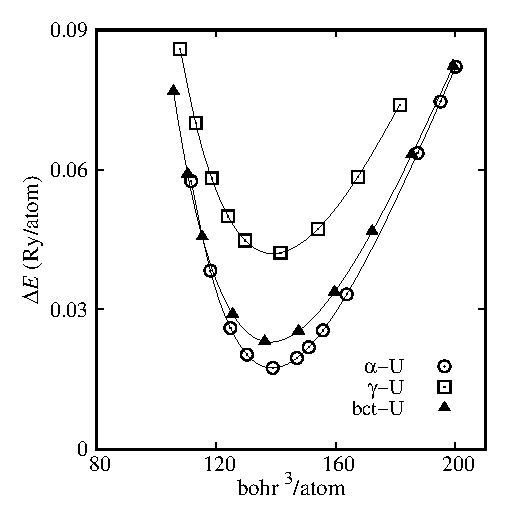
\includegraphics[width=4.3 in]{vol_en_u.eps}
	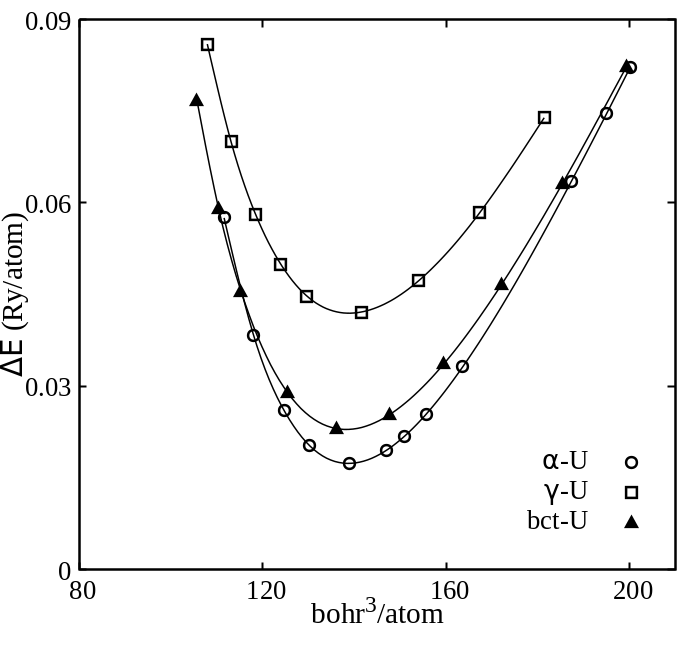
\includegraphics[width=4.3 in]{vol_en_u.png}
	\caption{Energy vs. volume curve for three different phases of uranium.}
	\label{fig:envsvolu}
\end{figure}

According to our calculations, \textalpha~phase has the lowest energy (see Fig.~\ref{fig:envsvolu}) at ground state. Properties of several uranium phases as calculated with the pseudopotential
presented above are detailed in the rest of this section.


\subsection{\boldmath \textalpha-Uranium} \label{subsec_alphaU}
Uranium's \textalpha\ phase has a base-centered orthorhombic structure with
space group \textit{Cmcm} (no.~63). The asymmetric unit has uranium atoms at
Wyckoff position $4c$ $\Bigl(0, \pm y, \pm\frac{1}{4}\Bigr)$, where the
position parameter $y$ has been found to be a function of
temperature~\cite{barrett1963crystal}.
At room temperature, the value of $y$ has been measured to be
0.1024~\cite{barrett1963crystal,lander1994solid}. There are four atoms in the
standard unit cell (two in the primitive cell).
%(A20 \textit{Strukturbeircht}) designation and oC4 Pearson symbol.
The \textalpha\ phase is thermodynamically favorable at temperatures below
935~K and pressures up to 100~GPa~\cite{le2003structural,akella1997structural}.
This makes the \textalpha\ phase important to the nuclear energy community
because it is the naturally-occurring phase of uranium. The solid-state physics
community also shows interest in \textalpha-uranium because of certain unusual
characteristics, including charge density wave transitions and
superconductivity.

The total energy as a function of unit cell volume for \textalpha-uranium is
shown in Figure~\ref{fig:alpha}; Table~\ref{table:eq_al} summarizes the
optimized lattice parameters, the distance parameter $y$, and the calculated
elastic moduli, along with results from previously-published calculations
and experiments. We confirm that \textalpha-uranium is the lowest-energy crystal
structure among those we tested. Our pseudopotential predicts an equilibrium
volume of 20.49~\AA$^3$, which is in close agreement with the experimental
value of 20.530~\AA$^3$ (at 50~K)\@. The position parameter $y$ exhibits a
minimum-energy 
value of 0.0986 at the equilibrium volume of 20.49~\AA$^3$.
This trend in $y$ is similar to that observed in the calculations of
Wills and Eriksson~\cite{wills1992crystal}.

Our cell volume results differ from previous calculations using
PAW~\cite{beeler2013first}, which obtained an equilibrium volume of
19.987~\AA$^3$ (the work was done using VASP~\cite{kresse1993ab, Kresse1996a, Kresse1996b}). A Murnaghan~\cite{murnaghan1944compressibility} fit to the
total energy as a function of volume for \textalpha-uranium yielded a bulk
modulus of 132.1~GPa, which is larger than the experimental value of
$104 \pm 2$~GPa~\cite{le2003structural},
but agrees closely with the quantum molecular dynamics (QMD) results of
Hood \etal~\cite{hood2008quantum} (133.5 GPa)
and the diamond anvil cell (DAC) experiments of Yoo \etal~\cite{yoo1998phase},
which reported a bulk modulus of 135.5~GPa. Our pseudopotential-based results
are in close agreement with the all-electron FP-LMTO calculations of
S{\"o}derlind~\cite{soderlind2002first}, which gave an equilibrium volume of
20.67~\AA$^3$ and a bulk modulus of 133.0~GPa. A published PAW-based
pseudopotential from Beeler \etal~\cite{beeler2013first} yields an equilibrium
volume of 19.92~\AA$^3$, which is lower than our result and farther from both
the experimental value and the result from all-electron calculations.

\begin{figure}
	\centering
    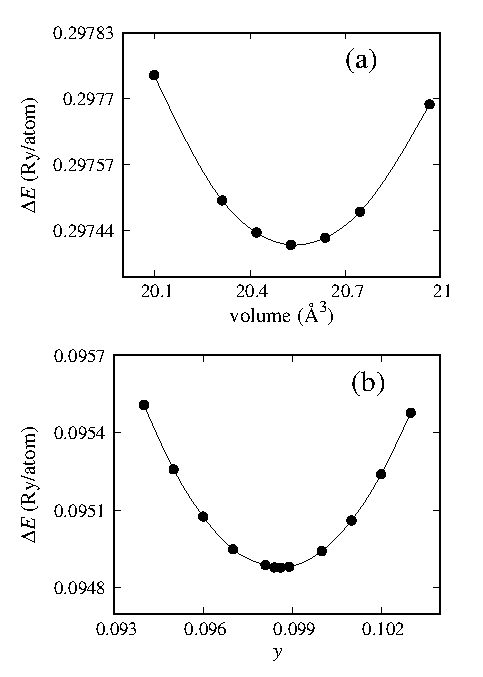
\includegraphics[width=4.25in]{twoPlots_alphaU}
    \caption[(a)~Calculated total energy as a function of volume for
        \textalpha-uranium. (b)~Calculated total energy as a function of the
        positional parameter $y$ for \textalpha-uranium.]{(a)~Calculated total energy as a function of volume for
        \textalpha-uranium. (b)~Calculated total energy as a function of the
        positional parameter $y$ for \textalpha-uranium. The calculation of $y$
        is constrained to an equilibrium volume of 20.49~\AA$^3$.}
	\label{fig:alpha}
\end{figure}

\begin{sidewaystable} 
%\begin{table}
%\small
%\label{table:eq_al}
\centering
\caption[Ground-state properties and elastic moduli of \textalpha-uranium from present work, compared with the PAW pseudopotential calculations of Beeler]{Ground-state properties and elastic moduli of \textalpha-uranium from present work, compared with the PAW pseudopotential calculations of Beeler \etal~\cite{beeler2013first}, the full-core calculations of S{\"o}derlind~\cite{soderlind2002first}, and experiments from Barrett~\cite{barrett1963crystal}, Le Bihan \etal~\cite{le2003structural}, and Fisher and McSkimin~\cite{fisher1958adiabatic}~(295~K).}
\label{table:eq_al}
%\begin{ruledtabular}
\begin{tabular}{cccccccc}
  \toprule
    & \multicolumn{3}{c}{Theory}
    && \multicolumn{3}{c}{Experiment} \\
    \cline{2-4}\cline{6-8}
				 & present work  & Beeler~\cite{beeler2013first}  & S{\"o}derlind~\cite{soderlind2002first} && Barrett~\cite{barrett1963crystal} & Le Bihan~\cite{le2003structural} & Fisher~\cite{fisher1958adiabatic} \\ \midrule 
$a$ (\AA)		 & 2.834		 & 2.793		 & 2.845	&&	2.836	& 2.8553 & -	\\
$b$ (\AA)		 & 5.862		 & 5.849		 & 5.818	&&	5.867	& 5.8702 & -	\\
$c$ (\AA)		 & 4.932		 & 4.893	     & 4.996	&&	4.936	& 4.9568 & -	\\
$y$ 			 & 0.0986		 & 0.097		 & 0.103	&&	0.102	& 0.102	 & -	\\
volume/atom (\AA$^3$) & 20.48		 & 19.987		 & 20.674	  && 20.535	& 20.770 & -	\\ 
$B$ (GPa)		 & 132.1		 & 151			 & 133		  && -		& 104(2) 	& -	\\
$B'$			 & 5.27			 & -			 & 5.4		  && -		&6.2		& -	\\
$C_{11}$ (GPa)		 & 315			 & 299			 & 300		  &&	-		&-		& 215 \\
$C_{22}$ (GPa)		 & 213			 & 231			 & 220		  &&	-		&-		&199 \\
$C_{33}$ (GPa)		 & 387			 & 364			 & 320		  &&	-		&-		&267 \\
$C_{44}$ (GPa)		 & 135			 &100			 & 150		  &&	-		&-		&124 \\
$C_{55}$ (GPa)		 & 87			 & 150			 & 93		  &&	-		&-		&73 \\
$C_{66}$ (GPa)	     & 104			 & 132			 & 120		  &&	-		&-		&74\\
$C_{12}$ (GPa)		 & 58			 & 59			 & 50		  &&	-		&-		&46\\
$C_{13}$ (GPa)		 & 45			 & 30			 & 5		  &&	-		&-		&22\\
$C_{23}$ (GPa)		 & 146			 & 144			 & 110		  &&	-		&-		&108\\
  \bottomrule
\end{tabular}
%\end{ruledtabular}
%\end{table}
\end{sidewaystable}



The elastic moduli predicted by our pseudopotential are
presented in Table~\ref{table:eq_al}. Like all materials with
orthorhombic symmetry, \textalpha-uranium has nine unique elastic
moduli. Our model overestimates most of the elastic moduli
relative to experiments. The three primary-direction elastic
moduli ($C_{11}$, $C_{22}$, and $C_{33}$) show good agreement
with other theoretical results and with experiment, though all
three principal elastic moduli are overestimated.
The order ($C_{33} > C_{11} > C_{22}$) of these three elastic
moduli is also consistent with experiments. For $C_{55}$ and
$C_{13}$, the present results also show good agreement with
experiments.  The value of $C_{66}$ is overestimated relative to
experiment, but closer than any existing prediction from a
pseudopotential-based calculation. The other elastic moduli are
generally similar to existing theoretical predictions.

\subsection{\textgamma-U: Crystal Structure and Elastic Moduli}
\label{subsec_gamma}

\begin{sidewaystable}
%\label{table_eq_gamma}
\centering
\caption[Equilibrium lattice parameters, volume per atom, and elastic moduli of \textgamma-uranium.]{Equilibrium lattice parameters, volume per atom, and elastic moduli of \textgamma-uranium. Results are compared with the PAW pseudopotential calculations from PsL~\cite{pp1,dal2014pseudopotentials},  Beeler \etal~\cite{beeler2013first}, and Taylor~\cite{taylor2008evaluation}, as well as the norm-conserving pseudopotential calculations of Crocombette \etal~\cite{crocombette2001plane} and the experiments of Wilson and Rundle~\cite{wilson1949structures} at room temperature. Elastic moduli are compared with previous PAW pseudopotential calculations from Beeler \etal~\cite{beeler2013first} and Taylor~\cite{taylor2008evaluation}.}
\label{table_eq_gamma}
%\hspace{-2cm}
%\begin{ruledtabular}
%\footnotesize
\begin{tabular}{ccccccccc}
  \toprule
  & \multicolumn{5}{c}{Theory} && \multicolumn{2}{c}{Experiment} \\
  \cline{2-6}\cline{8-9}
			& present work & PsL~\cite{pp1,dal2014pseudopotentials} & Beeler~\cite{beeler2013first} & Taylor~\cite{taylor2008evaluation} & Crocombette~\cite{crocombette2001plane} && Wilson~\cite{wilson1949structures} & Yoo~\cite{yoo1998phase} \\ \midrule
\rule{0pt}{2.2ex}%  
$a$~(\AA)			&   3.45 & 3.458  & 3.427	& 3.43	 & 3.37		   && 3.47	&-			\\		
volume/atom~(\AA$^3$) & 20.56 & 20.675 & 20.124	& 20.18	 & 19.14	   && 20.89	&-			\\ 
$C_{11}$ (GPa) &	28	& 27   & 86		& 161	 & -	&&-	&-	\\ 
$C_{12}$ (GPa) &	167	& 165  & 155	& 184	 & -	&&-	&-	\\
$C_{44}$ (GPa) &   51	&59	   & 37		& 56	 & -	&&-	&-	\\ 
$B$ (GPa)		&  121	&119   & 132	& 176	 & 170	&&-	& 113.3	\\ \bottomrule
\end{tabular}
%\end{ruledtabular}
\end{sidewaystable}


The structure of \textgamma-uranium at high temperature was first
elucidated by Wilson and Rundle~\cite{wilson1949structures} at Iowa
State University in 1949 using powdered uranium at
800~\textdegree C\@. The \textgamma~phase of uranium has a
body-centered cubic (bcc; Structurbericht designation A2) structure
with two atoms in the standard unit
cell~\cite{yakel1973review,nashchemistry}.
%(space group $Im\overline{3}m$)
It is thermodynamically stable from 1050~K to the melting point of
1406~K~\cite{yoo1998phase}.

In the nuclear fuels community, \textgamma-uranium is preferred to
\textalpha-uranium because it undergoes isotropic thermal expansion
and radiation-induced swelling~\cite{kittel1993history}. 
As Wilson and Rundle observed~\cite{wilson1949structures},
it is not possible to quench pure \textgamma-uranium to room
temperature, but a metastable bcc phase can be retained at room temperature
in U--Mo alloys.
Recently, it was found that the bcc structure can be retained by alloying
uranium with other metals, such as platinum, palladium, niobium, and
zirconium~\cite{kim2016superconductivity}.
In particular, the eutectoid point of \textgamma-uranium with molybdenum
impurities is at approximately 89~weight-percent uranium (see Fig.~\ref{fig:umophase}); to take advantage of
the depressed phase transition temperature (and the associated increase in
stability of the bcc phase), uranium alloyed with 10~wt\% molybdenum
($\approx$\,21.6 at.\%; U-10Mo) is currently being developed as a potential
high-density low-enrichment uranium (LEU) fuel for high-performance research
reactors. The lattice parameters, volume per atom, and elastic moduli as
calculated with our pseudopotential-based model are presented in
Table~\ref{table_eq_gamma}.

The lattice parameters for \textgamma-uranium as calculated with the
pseudopotential presented here are in good agreement with experiments.
The elastic moduli are comparable with those of
Beeler \etal~\cite{beeler2013first} and Taylor~\cite{taylor2008evaluation}.
The value of $C_{12}$ is larger than that of $C_{11}$, which is
a violation of one of the stability criteria for cubic crystals
$(C_{11}-C_{12} > 0)$, often called the Born stability
criterion~\cite{born1940stability,born1954dynamical,Mouhat2014}. This violation
is expected, as the bcc phase of uranium is unstable at low temperatures. The
experimental value of bulk modulus by Yoo \etal~\cite{yoo1998phase} is in good
agreement with our result.

\subsection{Body-Centered Tetragonal Uranium}
\label{subsec_bct}

\begin{table}
%\label{table:eq_bct}
\caption[The optimized lattice parameters (\AA), volume per atom (\AA$^3$) and elastic moduli of bct uranium.]{The optimized lattice parameters (\AA), volume per atom (\AA$^3$), and elastic moduli of bct uranium. Our calculated results are compared with those of Beeler \etal~\cite{beeler2013first}, Li \etal~\cite{li2012structure},
Xiang \etal~\cite{xiang2008quantum}, and S\"oderlind~\cite{Soderlind1998}.}
\label{table:eq_bct}
%\begin{ruledtabular}
\begin{tabular}{cccccc}
  \toprule
		& present work & Beeler~\cite{beeler2013first} & Li~\cite{li2012structure} & Xiang~\cite{xiang2008quantum} & S\"oderlind~\cite{Soderlind1998} \\ \midrule
$a$ (\AA)		&   3.44	   & 3.695	& 3.72 & - & -\\
$c/a$	&	0.8125	   & 0.8	& 1.24 & - & 0.82 \\
vol./atom (\AA$^3$)& 20.44	   & 20.268 & 31.896 & 20.5 & - \\
$C_{11}$ (GPa) &  270		   & 264	& 230 & - & -	\\
$C_{33}$ (GPa) &  257		   & 254	& 204 & - & -	\\
$C_{12}$ (GPa) &  65		   & 55		& 61 & - & -	\\
$C_{13}$ (GPa) &	32		   & 68		& 61 & - & -	\\
$C_{44}$ (GPa) &	59		   & 56		& 79 & - & -	\\
$C_{55}$ (GPa) &	71		   & 56		& 39 & - & - \\
$B$ (GPa)    &	115.4	   & 130	& 114  & - & - \\
  \bottomrule
\end{tabular}
%\end{ruledtabular}
\end{table}
The \textbeta~phase of uranium is stable at atmospheric pressure between 935
and 1045~K~\cite{lawson1988structure}.
Tucker~\cite{tucker1950approximate} determined that it has a tetragonal
structure with 30~atoms per unit cell, but his space group assignment was
later disputed. The assignment of a space group remained a controversy until
1988, when Lawson and coworkers~\cite{lawson1988structure} published neutron
powder diffraction results.
The experimental difficulties lie in the preparation of a single crystal of
\textbeta-uranium and the need to operate at high temperature.
Single crystals of a \textbeta-uranium alloy containing 1.4~atom\% chromium
were created by Tucker~\cite{tucker1951crystal} and quenched to room
temperature, but he did not establish whether this alloy had the same crystal
structure as pure \textbeta-uranium~\cite{lawson1988structure}. An overview of
the development of the crystal structure of \textbeta-uranium is given by
Donohue and Einspahr~\cite{donohue1971structure, donohue1974structures}. The
present consensus is that \textbeta-uranium has a tetragonal crystal structure
with with space group $P4_2/mnm$ (no.~136) and 30~atoms in the unit cell.

We chose to simulate a body-centered tetragonal structure instead of
\textbeta-uranium because of the latter's complexity and computational expense.
A similar simplification was used in studies similar to
ours~\cite{beeler2013first,li2012structure}.
The bct structure has only two atoms per unit cell, and is therefore less
computationally expensive than \textbeta-uranium.
The equilibrium lattice parameters of bct~uranium are presented in
Table~\ref{table:eq_bct}, alongside values from Beeler
\etal~\cite{beeler2013first} and Li \etal~\cite{li2012structure}.
The volume per atom agrees well with Beeler \etal\ but is significantly
different from that of Li \etal.
Xiang \etal~\cite{xiang2008quantum} also studied the bct structure of uranium,
though they did not provide the equilibrium lattice parameter or $c/a$ ratio;
their value of the equilibrium volume per atom was 20.5~\AA$^3$, similar but
larger than our value. Our $c/a$ ratio is in good agreement with
both Beeler \etal~\cite{beeler2013first} (0.8) and
S\"oderlind~\cite{Soderlind1998} (0.82).

\subsection{Face-Centered Cubic Uranium}
\label{subsec_fcc}

\begin{table}
%\label{table:eq_fcc}
\caption[The equilibrium lattice parameter, volume per atom, and elastic moduli
of fcc uranium.]{The equilibrium lattice parameter, volume per atom, and elastic moduli
of fcc uranium. Results are compared with PAW pseudopotential calculations of
Beeler \etal~\cite{beeler2013first}, Taylor~\cite{taylor2008evaluation}, and
Crocombette \etal~\cite{crocombette2001plane}.}
\label{table:eq_fcc}
%\begin{ruledtabular}
\begin{tabular}{cccccc}
  \toprule
				   & present work & Beeler~\cite{beeler2013first} & Taylor~\cite{taylor2008evaluation} & Crocombette~\cite{crocombette2001plane} \\ \midrule
$a$ (\AA)				   & 4.300  		  & 4.433	& 4.48	 & 4.30				\\
volume/atom (\AA$^3$)	   & 21.765   & 21.774	& 22.48  & 19.88			\\ 
$C_{11}$ (GPa) &  	67			& 46	 & 184 &-	  \\
$C_{12}$ (GPa) &	130			& 144	 & 267 &-	  \\
$C_{44}$ (GPa) &	38			& 40	 & 28  &-   \\
$B$ (GPa)		&	108.7		& 111	 & 239	&148	\\
  \bottomrule
\end{tabular}
%\end{ruledtabular}
\end{table}
Face-centered cubic uranium does not exist in nature, but it is a reasonable
way to check the pseudopotential. Beeler \etal~\cite{beeler2013first} and
Taylor~\cite{taylor2008evaluation} studied this structure as well, so we
compare our results with theirs.
Table~\ref{table:eq_fcc} shows the equilibrium parameters and elastic moduli
as calculated with our model and with several other published pseudopotentials.
Our results are in good agreement with other pseudopotential calculations,
particularly those of Beeler \etal~\cite{beeler2013first};
the bulk modulus shows good agreement with their value as well.
It should be noted that $C_{12}$ is still higher than $C_{11}$, confirming that this model predicts the fcc phase to be unstable.

\subsection{Electronic Density of States}
\begin{figure}
	\centering
	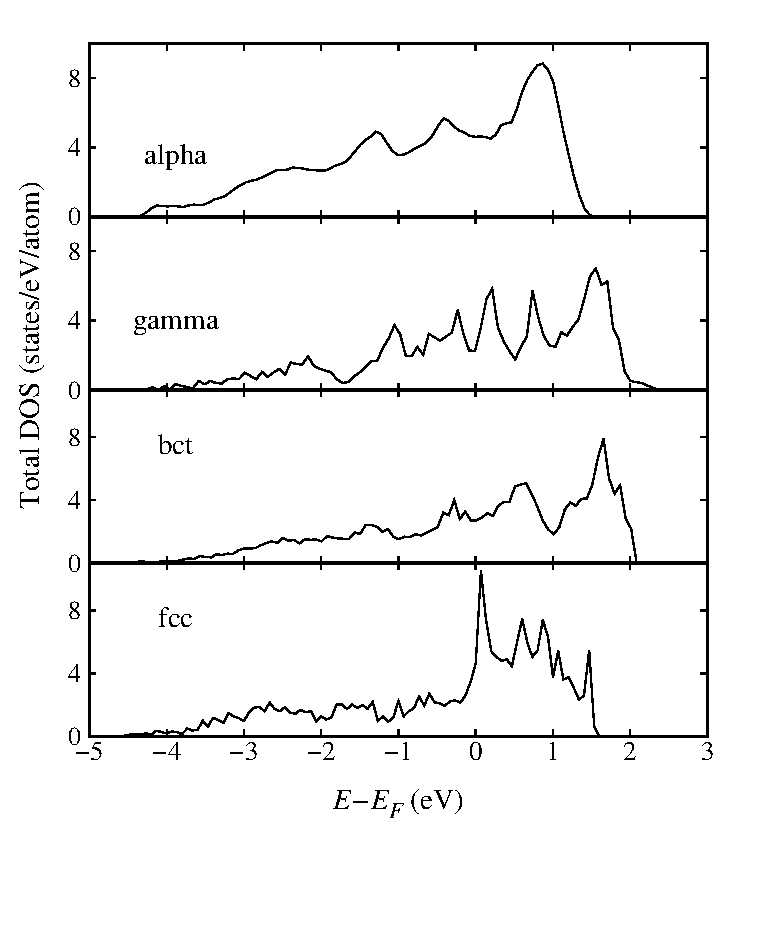
\includegraphics[width=4.8in]{total_DOS_allU}
    \caption{Total electronic densities of states of \textalpha, \textgamma,
      bct, and fcc uranium near the Fermi level.}
	\label{fig:totDos}
\end{figure}

\begin{figure}
	\centering
	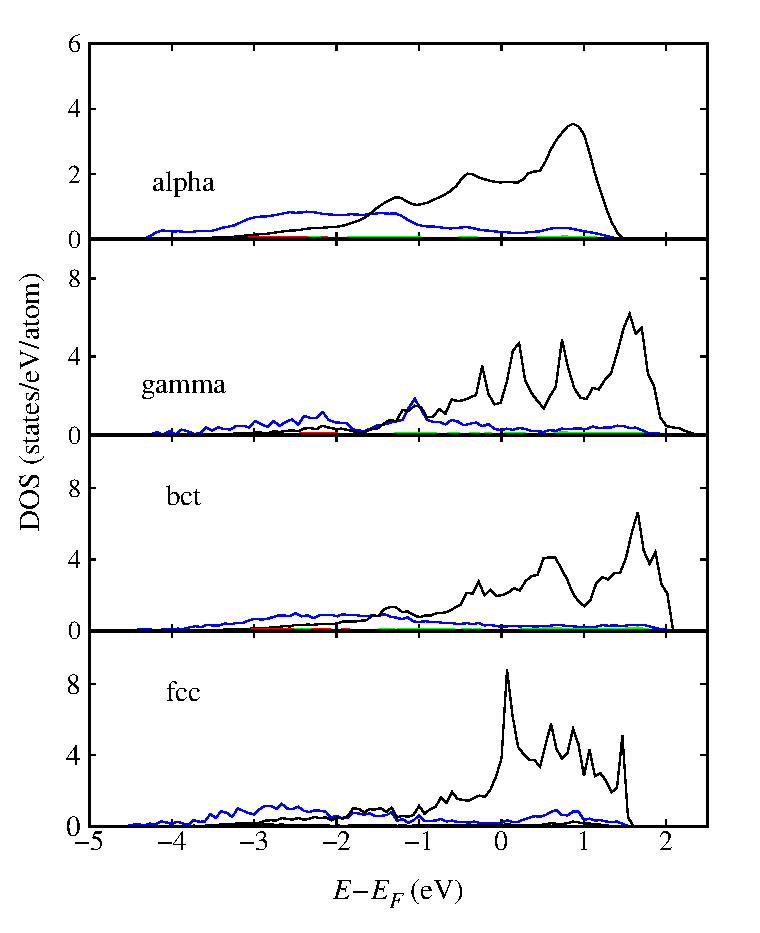
\includegraphics[width=4.8in]{spdf_orbital}
    \caption[The partial electronic densities of states of \textalpha,
      \textgamma, bct, and fcc uranium near the Fermi level.]{The partial electronic densities of states of \textalpha,
      \textgamma, bct, and fcc uranium near the Fermi level. The $6d$ (blue
      line) and $5f$ (black line) electronic orbitals are shown. The $s$ (red)
      and $p$ (green) electronic orbitals are also included, but due to their
      very low contributions near the Fermi level, they are barely visible.}
	\label{fig:fdorbitals}
\end{figure}

The electronic densities of states (DOS) of \textalpha, bct, \textgamma, and
fcc uranium are shown in Figure \ref{fig:totDos}. The partial densities of
states for the $5f$ and $6d$ orbitals are shown in Figure~\ref{fig:fdorbitals}.
We have only shown the partial densities of states for the $5f$ and $6d$
orbitals because these are the dominant orbitals near the Fermi level of
uranium. There are also contributions from $6s$, $6p$, and $7s$ orbitals near
the Fermi level, but these contributions are not as significant as the dominant
$5f$ and $6d$ orbitals.
%At the Fermi level, the dominant electronic contributions are from the $5f$
%orbitals, though the $6d$ orbitals do contribute.
Electrons near the Fermi level
are important because they are responsible for most of the metallic behavior.
From Figure~\ref{fig:totDos}, it can be seen that the DOS spreads over energies
between $-4$~eV and 2~eV relative to the Fermi level. The density of states
with our model is comparable to those calculated by Beeler
\etal~\cite{beeler2013first} and Xiang \etal~\cite{xiang2008quantum}.
For bcc and bct uranium, the $f$ orbitals spread over a broader range of
energies near the Fermi level and show multiple peaks above the Fermi level.
The high density of states at energies above the Fermi level in the bct
and \textgamma\ phases suggests that these phases would be favored over
\textalpha-uranium at high temperature.

\section{Conclusion}
The equilibrium structures, cell volumes, and elastic moduli have been
calculated using DFT with a newly-parameterized pseudopotential model for four
different uranium phases (\textalpha, \textgamma, body-centered
tetragonal, and face-centered cubic). Our results are either in good agreement
with previous work or show improvement in comparison with experiments.
Studying pure uranium is the first step in exploring different alloys of
uranium that are of interest to the nuclear fuels community.
Due to the lower cutoff energies that can typically be used, PAW-based
pseudopotentials allow one to study larger supercells, which in turn provide
more accurate studies of vacancy formation, grain boundaries, and fission gas
transport.

According to our pseudopotential, \textalpha-uranium is the lowest-energy
crystal structure of the ones tested.
The calculated elastic moduli show good agreement with previous DFT studies
and experiments. Our model shows good agreement with previous pseudopotentials,
but generally provides results that are either comparable to previously
published pseudopotentials or closer to experimental values than previously
published pseudopotentials.
The three elastic moduli associated with shear ($C_{44}$, $C_{55}$, and
$C_{66}$) show better agreement with experimental results than the tensile
components. The lattice parameters of the bct structure are also very similar
to those predicted by Beeler \etal~\cite{beeler2013first}, but they deviate
significantly from those of Li \etal~\cite{li2012structure}.
The elastic moduli show very similar trends to previously-published models,
apart from $C_{23}$, which is over-predicted by our model.

For \textgamma-uranium, which is of great interest for the development of
low-enrichment uranium fuel, the lattice parameters are in close agreement with
those of of Taylor \etal~\cite{taylor2008evaluation} and with experiments.
Apart from the elastic modulus $C_{11}$, the values of all computed parameters
show very little discrepancy compared with those from the work of Taylor
\etal~\cite{taylor2008evaluation} and Beeler \etal~\cite{beeler2013first}.
The bulk modulus shows very good agreement with experiment.

For fcc uranium, a hypothetical crystal structure, the computed lattice
parameter is in close agreement with values reported by Beeler
\etal~\cite{beeler2013first} and by Crocombette
\etal~\cite{crocombette2001plane}. The equilibrium volume per atom does show a
discrepancy from Crocombette but is in good agreement with Beeler \etal.
The elastic modulus $C_{44}$ is also in good agreement with Beeler \etal,
whereas $C_{11}$ is intermediate between the value predicted by Beeler \etal\
and that predicted by Taylor \etal.
Lastly, the electronic density of states shows that the $5f$
orbital partial density of states is the largest contribution to the total
density of states at the Fermi energy, and the $5f$ electrons therefore
contribute the most to the bonding and conductivity of uranium. Most of the
$5f$ orbital electron density is spread over energies between $-4$ and 2~eV
relative to the Fermi level. We also find that \textgamma-uranium has the
highest density of states at energies above the Fermi level, confirming that it
should be favored at high temperature.

%\appendixname
\newpage
\addcontentsline{toc}{section}{\protect\numberline{}Appendix: Elastic Parameter Calculation of \textalpha-uranium}\label{appen_elalpha}
\section*{Appendix: Elastic Parameter Calculation of \boldmath $\alphaup$-uranium}
In this appendix, we will discuss the stress-strain relationships that were used to calculate the nine independent elastic constants of \textalpha-uranium. The base-centered orthorhombic phase of uranium has three lattice parameters: $a$, $b$, and $c$; with the Bravais lattice matrix
\begin{equation}\label{eq_lattic_alphaU}
\mathbf{R} = \begin{bmatrix}
			\frac{a}{2} & -\frac{b}{2} & 0 \\
			\frac{a}{2} & \frac{b}{2} & 0 \\
			0			&    0        & c 
			\end{bmatrix}.
\end{equation}
Applying a small strain to the equilibrium lattice changes the total energy, and from this information, the elastic parameters are deduced. The elastic parameters are identified as proportional to the second order coefficient in a polynomial fit of the total energy as a function of the distortion parameter $\delta$~\cite{wallace1998thermodynamics}. The distortion of the lattice vectors follows the rule $\mathbf{R'}=\mathbf{RD}$. Here, $\mathbf{R'}$ is a matrix containing the components of the distorted lattice vectors and $\mathbf{D}$ is the symmetric distortion matrix.



The internal energy of a crystal under strain $\delta$ can be expanded in powers of the strain tensor with respect to initial energy of the unstrained crystal in the following way:
	\begin{equation}
	\label{eq_taylor_el}
	E(V,\delta) = E(V_0,0) + V_0 \left ( \sum_i \tau_i \xi_i d_1 + 1/2 \sum_{ij} C_{ij} \delta_i \xi_i \delta_j \xi_j \right ) + \mathcal{O}(\delta^3) 
	\end{equation}
The unstrained volume is $V_0$, and $E(V_0,0)$ is the energy of the unstrained system. Voight notation has been used in Eqn.~\eqref{eq_taylor_el} (\ie, $xx$, $yy$, $zz$, $yz$, $xz$, and $xy$, respectively, are replaced with 1--6). Here, $yz$, $xz$, and $xy$, are equal to $zy$, $zx$, and $yx$, and for this reason, $\xi_i$ is equal to 1 for $i=1$, $2$, and $3$ and equal to $2$ for $i=4$, $5$, and $6$. $\tau_i$ is a component of the stress tensor. The first three elastic constants; $C_{11}$, $C_{22}$, and $C_{33}$; are obtained form the following distortions:
\begin{equation}
\label{eq_D1}
	\mathbf{D_1} =  \begin{bmatrix}
						1+\delta & 0 & 0 \\
						0 & 1 & 0 \\
						0 & 0 & 1 \\
						\end{bmatrix}
\end{equation}

\begin{equation}
\label{eq_D2}
	\mathbf{D_2} = \begin{bmatrix}
						1 & 0 & 0 \\
						0 & 1+\delta & 0 \\
						0 & 0 & 1 \\
					\end{bmatrix}
\end{equation}

\begin{equation}
\label{eq_D3}
\mathbf{D_3} =  \begin{bmatrix}
						1 & 0 & 0 \\
						0 & 1 & 0 \\
						0 & 0 & 1+\delta \\
						\end{bmatrix}.
\end{equation}
The internal energies for these three distortions can be obtained from 
\begin{equation}
\label{eq_d1d2d3}
E(V,\delta) = E(V_0,0) + V_0\tau_i \delta + \frac{V_0C_{ii}\delta^2}{2}.
\end{equation}
The constants $C_{44}$, $C_{55}$, and $C_{66}$ are related to the distortions:
\begin{equation}
\label{eq_D4}
	\mathbf{D_4} = \begin{bmatrix}
						\frac{1}{(1-\delta^2)^{1/3}} & 0 & 0 \\
						0 & \frac{1}{(1-\delta^2)^{1/3}} & \frac{\delta}{(1-\delta^2)^{1/3}} \\
						0 & \frac{\delta}{(1-\delta^2)^{1/3}} & \frac{1}{(1-\delta^2)^{1/3}} \\
						\end{bmatrix}
\end{equation} 

\begin{equation}
\label{eq_D5}
	\mathbf{D_5} =  \begin{bmatrix}
						\frac{1}{(1-\delta^2)^{1/3}} & 0 & \frac{\delta}{(1-\delta^2)^{1/3}} \\
						0 & \frac{1}{(1-\delta^2)^{1/3}} & 0 \\
						\frac{\delta}{(1-\delta^2)^{1/3}} & 0 & \frac{1}{(1-\delta^2)^{1/3}} \\
						\end{bmatrix}
\end{equation}
and
\begin{equation}\label{eq_D6}
						\mathbf{D_6} = \begin{bmatrix}
						\frac{1}{(1-\delta^2)^{1/3}} & \frac{\delta}{(1-\delta^2)^{1/3}} & 0 \\
						\frac{\delta}{(1-\delta^2)^{1/3}} & \frac{1}{(1-\delta^2)^{1/3}} & 0 \\
						0 & 0 & \frac{1}{(1-\delta^2)^{1/3}} \\
						\end{bmatrix}.
\end{equation}	
These three elastic constants can be calculated from the corresponding internal energy:
\begin{equation}
							E(V,\delta) = E(V_0,0) + V_0\tau_i \delta + \frac{V_0C_{ii}\delta^2}{2}
\end{equation}
The last three distortions are
\begin{equation}\label{eq_D7}
						\mathbf{D_7} = \begin{bmatrix}
						\frac{1+\delta}{(1-\delta^2)^{1/3}} & 0 & 0 \\
						0 & \frac{1-\delta}{(1-\delta^2)^{1/3}} & 0 \\
						0 & 0 & \frac{1}{(1-\delta^2)^{1/3}} \\	
						\end{bmatrix}
\end{equation}			

\begin{equation}\label{eq_D8}
						\mathbf{D_8} =  \begin{bmatrix}
						\frac{1+\delta}{(1-\delta^2)^{1/3}} & 0 & 0 \\
						0 & \frac{1}{(1-\delta^2)^{1/3}} & 0 \\
						0 & 0 & \frac{1-\delta}{(1-\delta^2)^{1/3}} \\
						\end{bmatrix}
\end{equation}	
and
\begin{equation}\label{eq_D9}
						\mathbf{D_9} = \begin{bmatrix}
						\frac{1}{(1-\delta^2)^{1/3}} & 0 & 0 \\
						0 & \frac{1+\delta}{(1-\delta^2)^{1/3}} & 0 \\
						0 & 0 & \frac{1-\delta}{(1-\delta^2)^{1/3}} \\	
						\end{bmatrix}
\end{equation}
The internal energies related to these three distortions are given by the following equations:
\begin{gather}
E(V,\delta) = E(V_0, 0) + V_0\left [ \tau_1 - \tau_2 \right ] \delta + \frac{1}{2} \left(C_{11} + C_{22} -2C_{12}  \right)\delta^2 \\
E(V,\delta) = E(V_0, 0) + V_0\left [ \tau_1 - \tau_3 \right ] \delta + \frac{1}{2} \left(C_{11} + C_{33} -2C_{13}  \right)\delta^2 \\
E(V,\delta) = E(V_0, 0) + V_0\left [ \tau_2 - \tau_3 \right ] \delta + \frac{1}{2} \left(C_{22} + C_{33} -2C_{23}  \right)\delta^2
\end{gather}
The above equations can be used to calculate the remaining elastic constants $C_{12}$, $C_{13}$, and $C_{23}$\@. The energy and strain relations are calculated and included in Figures~\ref{fig_D123}, \ref{fig_D456}, and \ref{fig_D789}\@. 

\begin{figure}
	\centering
	\includegraphics[]{d123_alphaU.eps}
	\caption{Changes in the strain energy as a function of strain using distortion matrix~$D_1$~\eqref{eq_D1}, $D_2$~\eqref{eq_D2}, and $D_3$~\eqref{eq_D3}.}
	\label{fig_D123}
\end{figure}

\begin{figure}
	\centering
	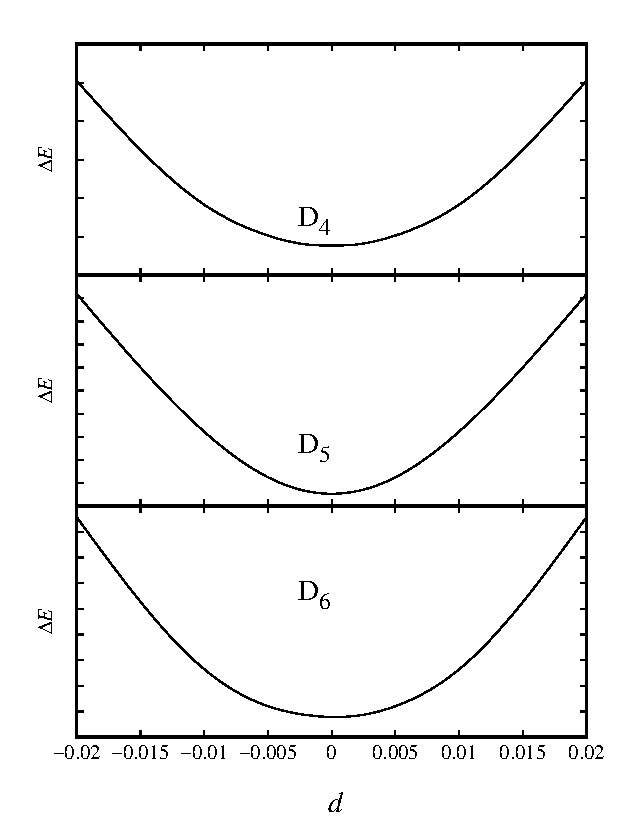
\includegraphics[]{d456_alphaU.eps}
	\caption{Changes in the strain energy as a function of strain using distortion matrix~$D_4$~\eqref{eq_D4}, $D_5$~\eqref{eq_D5}, and $D_6$~\eqref{eq_D6}.}
	\label{fig_D456}
\end{figure}

\begin{figure}
	\centering
	\includegraphics[]{d789_alphaU.eps}
	\caption{Changes in the strain energy as a function of strain using distortion matrix~$D_7$~\eqref{eq_D7}, $D_8$~\eqref{eq_D8}, and $D_9$~\eqref{eq_D9}.}
	\label{fig_D789}
\end{figure}

\clearpage
\addcontentsline{toc}{section}{\protect\numberline{}Appendix: Elastic Parameter Calculation for \textgamma-uranium}\label{appen_bccel}

\section*{Appendix: Elastic Parameter Calculation for \boldmath \textgamma-uranium}
Applying a small strain ($\delta$) to the equilibrium lattice changes the total energy, and from this information, the elastic parameters are deduced. The distortion of a lattice vector follows the rule $\mathbf{R'} = \mathbf{RD}$. Here, $\mathbf{R}$ is the Bravais lattice vector, $\mathbf{R'}$ is a matrix containing the components of the distorted lattice vectors, and $\mathbf{D}$ is the symmetric distortion matrix.


By symmetry, there are only three independent elastic parameters for a cubic system (\ie, $C_{11}, C_{12}$, and $ C_{44}$).
Elastic parameters are evaluated from the total energy of the crystal, to which volume-conserving orthorhombic $[C'=(C_{11} - C_{12})/2]$ and monoclinic $(C_{44})$ distortions are applied. The relevant distortion matrices are 
%\[\begin{bmatrix}
\begin{equation}
\mathbf{D_\text{ortho}} = \label{eq:ortho}
		\begin{bmatrix}
		1+\delta_o & 0 & 0 \\
		0 & 1-\delta_o & 0 \\
		0 & 0 & \frac{1}{1-\delta_o^2}\\
		\end{bmatrix}
\end{equation}
%\end{bmatrix} \]
and
\begin{equation}
\label{eq:mono}
\mathbf{D_\text{mono}} = \begin{bmatrix}
	1 & \delta_m & 0 \\
	\delta_m & 1 & 0 \\
	0 & 0 & \frac{1}{1-\delta_m^2} \\
\end{bmatrix}.
\end{equation}
The associated total energy change for an orthorhombic distortion is 
\begin{equation}
\label{eq_ortho}
\Delta E = V(C_{11} - C_{12})\delta_o^2 + \mathcal{O}(\delta_o^4) .
\end{equation}
For a monoclinic distortion, the energy change is
\begin{equation}
\label{eq_mono}
\Delta E = 2VC_{44}\delta_m^2 + \mathcal{O}(\delta_m^4).
\end{equation}

\begin{figure}
	\centering
	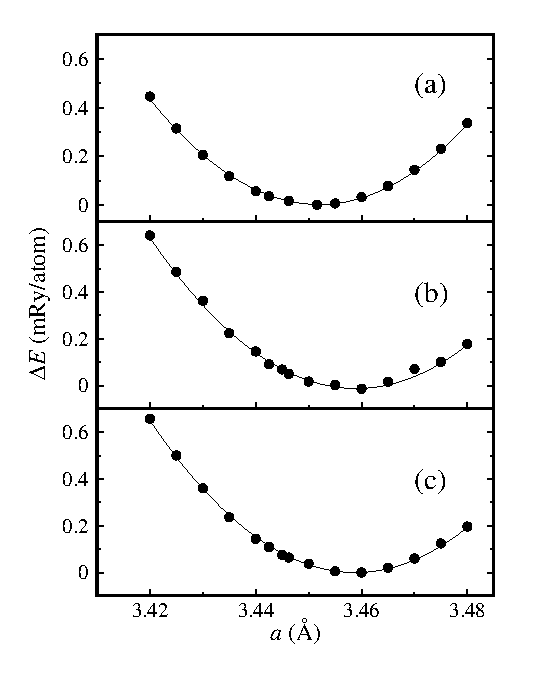
\includegraphics[width=4.25 in]{figure_bulk}
    \caption[Energy as a function of lattice parameter for \textgamma-uranium]{Energy as a function of lattice parameter for \textgamma-uranium. (a)~this work with a $k$-point mesh of $30\times30\times30$; (b)~Pseudopotential from PS library~\cite{dal2014pseudopotentials, pp1}
 with a $k$-point mesh of $30\times30\times30$; (c)~Pseudopotential from PS library~\cite{dal2014pseudopotentials, pp1}
 with $42\times42\times42$ $k$-point mesh.}
	\label{fig:bulkgamma}
\end{figure}

\begin{figure}
	\centering
	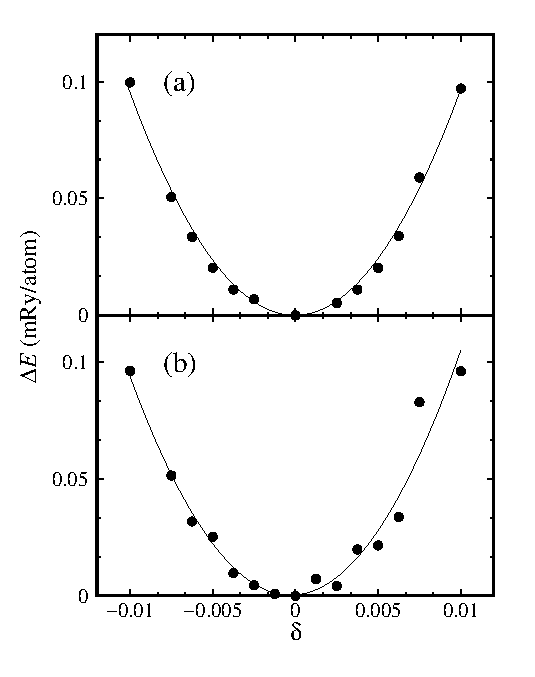
\includegraphics[width=4.25 in]{figure_mono}
    \caption[Changes in the strain energy as a function of strain $(\delta)$ for monoclinic distortions of \textgamma-uranium]{Changes in the strain energy as a function of strain $(\delta)$ for monoclinic distortions of \textgamma-uranium (Eq.~\eqref{eq:mono} and Eq.~\eqref{eq_mono}). (a)~this work; (b)~Pseudopotential from the PS library~\cite{dal2014pseudopotentials, pp1}. Increasing the number of $k$-points does not improve the smoothness of plot (b).}
\label{fig:monogamma}
\end{figure}

\begin{figure}
	\centering
	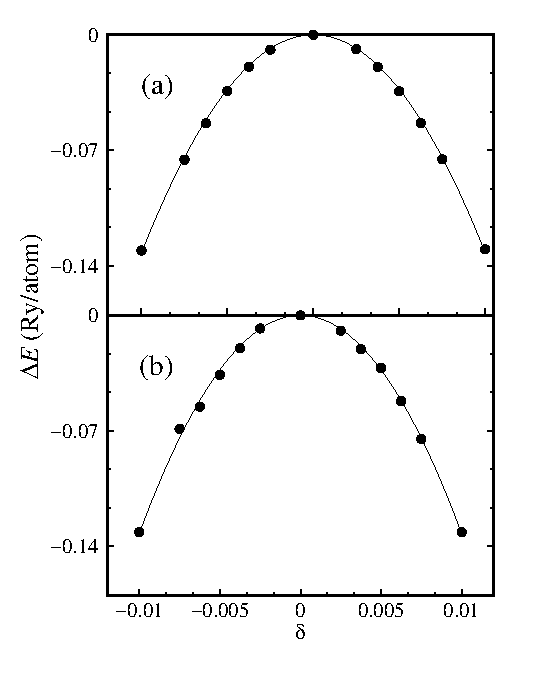
\includegraphics[width=4.25 in]{figure_ortho}
    \caption[Changes in the strain energy as a function of strain $(\delta)$ for orthorhombic distortions of \textgamma-uranium]{Changes in the strain energy as a function of strain $(\delta)$ for orthorhombic distortions of \textgamma-uranium (Eq.~\eqref{eq:ortho} and Eq.~\eqref{eq_ortho}). (a)~this work; (b)~Pseudopotential from the PS library~\cite{dal2014pseudopotentials, pp1}.}
	\label{fig:orthogamma}
\end{figure}



\clearpage
\bibliographystyle{apsrev4-2}
\bibliography{abbreviated,final}
%\bibliography{abbreviated,pseudo}


\chapter[Xenon Mobility in \protect\NoCaseChange{U--Mo} fuel]{Xenon Mobility in BCC-Uranium and Uranium--Molybdneum Alloys}
\textit{This chapter is based on work that will be submitted for publication to the Journal of Physics: Condensed Matter. The authors are A. Rafi M. Iasir and Karl D. Hammond of the University of Missouri.}



\section{Introduction}\label{sec_intro}
High performance research reactors require high-enrichment uranium (HEU) fuels
to attain the desired neutron flux. The replacement of HEU fuels with
low-enrichment uranium (LEU) is an important antiproliferation initiative. The
United States High-Performance Research Reactor (USHPRR) program is currently
aiming to replace the HEU fuels currently used in high performance reactors
with LEU fuels~\cite{snelgrove1997development}.
LEU fuels require a higher uranium density than that of uranium oxides
to compensate the decrease in \ce{^{235}U} enrichment.
Metallic uranium shows a great promise in this regard.

Metallic fuels are usually chosen because of their high thermal conductivity
and high density. Isotropic swelling behaviour is desirable, but uranium,
like other light actinides (Pa--Pu), has a low-symmetry crystal structure
(the orthorhombic \textalpha\ phase) at ambient temperature and pressure,
which results in anisotropic thermal and radiation-induced expansion.
%The influence of $5f$ electron--electron correlation plays an
%important role in the crystal structure of uranium and other light
%actinides~\cite{Soderlind1995,lander2003gh, freemanHandbook1984}.
%A narrow band of $5f$ states ($\approx$\,1--3~eV) goes through Peierls
%distortions~\cite{peierls1955} and favours an open, low-symmetry structure.
Pure uranium has three allotropes at atmospheric pressure:
\textalpha\ (base-centred orthorhombic), \textbeta\ (tetragonal), and
\textgamma\ (body-centred cubic). At atmospheric pressure, \mbox{\textalpha-U}
transforms to \mbox{\textbeta-U} at approximately 935~K, and \mbox{\textbeta-U}
transforms to \mbox{\textgamma-U} at approximately
1045~K~\cite{lawson1988structure,akella1997structural}. 

The \mbox{\textgamma-uranium} allotrope (which is body-centred cubic) is
preferred to \mbox{\textalpha-uranium} by nuclear engineers because it
undergoes both isotropic thermal expansion and isotropic radiation-induced
swelling~\cite{kittel1993history}.
It is not possible to quench pure \mbox{\textgamma-uranium} to room
temperature; however, a metastable bcc phase can be obtained at room
temperature by alloying with
molybdenum~\cite{wilson1949structures, sinha2010phase,
    yakel1969crystal,sinha2010effect}.
A study by Kim-Ngan and Havela~\cite{kim2016superconductivity} showed that the
bcc structure can also be retained at temperatures below the ordinary phase
transition temperature by alloying uranium with metals such as platinum,
palladium, niobium, and zirconium.
Molybdenum stabilises uranium's \textgamma\ phase at concentrations near the
eutectoid point (11.1 wt\% Mo) and lowers the phase transition temperature from
1045~K for pure \textgamma-uranium to 828~K for a U--Mo alloy at the eutectoid
point~\cite{ASM-Alloy-Mo,Berche2011}.
Uranium alloyed with 10~wt\% molybdenum (U-10Mo, which is approximately
21.6~at.\% molybdenum) is currently being developed as a potential
high-density, low-enrichment uranium fuel for high-performance research
reactors~\cite{prabhakaran2017u, meyer2014irradiation, williams2017post}.

Uranium--molybdenum alloys have been studied extensively both
experimentally~\cite{dwight1960uranium,tangri1961metastable, sinha2010phase}
and theoretically~\cite{berche2011calphad,zhang2010thermodynamic,
    losada2019ground, landa2011density,alonso2007role}.
Castellano \etal~\cite{castellano2020thermodynamic} showed that the
addition of molybdenum to uranium leads to the stabilisation of the
\textgamma\ phase using \textit{ab initio} molecular dynamics.
This thermodynamic stabilisation is important because un-alloyed
\textgamma-uranium would quickly revert back to \textalpha-uranium, causing high stresses and
cracking of the fuel and cladding. %The transition to $\alpha + \text{U}_2\text{Mo}$ happens more quickly in the irradiation environment.

Fission creates a variety of products, resulting in gas bubbles,
metallic precipitates, and solutes in the fuel matrix.
Among the many fission products, fission gas (\ie, xenon and krypton) produces
some of the most significant challenges associated with nuclear fuel
development. Fission gas influences the thermal conductivity,
causes swelling, and impacts the neutron economy of the
reactor~\cite{rondinella2010high,iasir2018estimation}. The ratio of xenon and krypton in fission gases is nine to one~\cite{rest2006u}. The important fission gas isotopes with short half lives are $^{133}$Xe (5.25 d) and $^{135}$Xe (9.1 h). Among them, $^{135}$Xe has a very high neutron absorption cross-section ($\sigma_a = \num{2.7e6}\pm 0.1$ barns) that can lower the fuel reactivity. Hence, the evolution of fission gases are directly related to the fuel performance. 

Large fission gas atoms (\ie, xenon) are mostly insoluble in the fuel matrix~\cite{grimes1991stability,andersson2011u}. There is a significant driving force for segregation of fission gas atoms to defects such as grain boundaries or dislocations and consequently form gas bubbles at these sinks.  Post irradiation analysis of U--Mo showed that, the fission gases distribute themselves inside the grain and grain boundaries~\cite{miller2012advantages, miller2015transmission, gan2010transmission, gan2012tem}. Fission gas in U--Mo alloys also forms superlattices, where they distribute themselves in an organised array~\cite{gan2012tem,van2008transmission}. To understand the mechanism, the rate-limiting steps of fission gas diffusion need to be studied. One of them is the individual gas atom movements through the fuel matrix using vacancies.
 %The atomic-scale transport processes in U--Mo alloys are of great interest to understand fuel performance during irradiation.
%Interestingly, molybdenum is itself a fission product.
%Specifically, the characteristics of fission gas are an important performance-limiting factor. 


The behaviour of fission gas
has been extensively researched for common fuels such as
\ce{UO2}~\cite{yun2008atomic,carter1972xenon,matzke1966diffusion,
    macewan1964xenon, une1987effects}.
A number of theoretical approaches have also been used to understand the
behaviour of fission products in \ce{UO2}, including electronic structure
theory~\cite{catlow1978fission,jackson1986calculation,grimes1989calculations,
    ball1990diffusion,grimes1991stability, petit1999location,
    crocombette2002ab, freyss2006ab, andersson2011u}.
In particular, vacancies play an important role in the diffusion of xenon
because of its size relative to the metal atoms.

Solute diffusion in light actinides is a very interesting phenomenon because
such solutes typically have very high diffusivities.
% FIXME Relative to...? Uranium self-diffusion?
Diffusion of solutes in metallic uranium has not been studied extensively.
However, there are some early works that provide some information about defect
and impurity diffusion in uranium~\cite{adda1959etude,peterson1964diffusion,
    rothman1959self, rothman1961diffusion, adda1962etude, resnick1962self,
    rothman1961self, liu2012atomic}.
Recently, Smirnova \etal~\cite{smirnova2015atomistic} studied self-diffusion in
\textgamma-uranium and U--Mo alloys using molecular dynamics.
They showed that diffusion in \textgamma-uranium is anomalously fast compared
to other bcc metals.

In recent years, there have been many attempts to calculate diffusion
coefficients using electronic structure and atomistic
methods~\cite{adams1989self, blochl1993first, blochl1990first, frank1996first,
    janotti2004solute, krvcmar2005diffusion, milman1993free, sandberg2002self}.
Electronic structure calculations based on DFT and multi-frequency models have
shown their usefulness in various works.
Five-frequency models of face-centred cubic
    crystals~\cite{lidiard1955,lidiard1960, leclaire1956} and
nine-frequency (or sometimes four-frequency) models of bcc
crystals~\cite{leclaire1970, mehrer2007diffusion} have been widely used.
Methods based on electronic structure theory involve calculating the activation
energies of an atom jumping to a vacancy in one of the atom's nearest-neighbour
positions. This is often referred to as vacancy-mediated diffusion.
The calculations employed here are based on DFT coupled with classical
transition state theory (TST), which treats vibration using the
harmonic oscillator
approximation~\cite{vineyard1954theory, vineyard1957frequency}.

In this study, we use DFT and TST to study the diffusion of xenon and
molybdenum in \textgamma-uranium alloys such as U--7Mo and U--10Mo by varying the local molybdenum concentration around the diffusing solute atom.
We find that molybdenum's migration energy is much higher than xenon's in
\textgamma--U alloys and that the presence of molybdenum in the local
environment of a xenon atom tends to
decrease the mobility of xenon in \textgamma-uranium alloys.
We also calculate the vacancy--solute binding energies of several solutes
in \textgamma-uranium and find that such binding energies are generally
higher in \textgamma-uranium than in iron or aluminium.



\section{Theory}\label{sec_theory}
Diffusion coefficients in crystalline solids are often described by an
Arrhenius equation over a wide range of temperatures. This model consists of
two parameters, the migration energy, $E_m$, and the pre-exponential factor,
$D_0$, with the diffusion coefficient given by
\begin{equation}
    D = D_0 e^{-E_m/k_B T},
\end{equation}

\nomenclature{$D$}{diffusion coefficient}
\nomenclature{$D_0$}{pre-exponential factor}
\nomenclature{$E_m$}{migration energy}
\nomenclature{$Q_{\text{IS}}$}{vibrational partition function of the initial state}
\nomenclature{$Q_{\text{TS}}$}{vibration partition function of transition state}


where $k_B$ is the Boltzmann constant and $T$ is the absolute temperature.
If $D_0$ is independent of temperature, an Arrhenius plot ($D$ against $1/T$)
gives a straight line; if $D_0$ changes with $T$, it yields a curve that falls
away from the constant-$D_0$ line at high temperature (the left of the plot).

The migration energy is the activation energy for an atom to jump onto a
nearby vacancy. According to classical transition state theory (TST), the rate
at which a vacancy exchanges its place with neighbouring atom can be expressed
by the Eyring--Polanyi
equation~\cite{Eyring1935,Evans1935,vineyard1957frequency},
\begin{equation}
    v = \nu^\ddagger \exp\left(\frac{-\Delta G_m}{k_B T}\right)
      \approx \frac{k_B T}{h} \frac{Q_\text{TS}}{Q_\text{IS}}
              \exp\left(\frac{-E_m}{k_B T}\right)
      \approx \frac{k_B T}{h}
              %\left[
              %\frac{\displaystyle\prod_{i=1}^{3N-3} \nu_i}
              %     {\displaystyle\prod_{j=1}^{3N-4} \nu_j^\ddagger}
              %\right]
              \exp\left(\frac{-E_m}{k_B T}\right),
\end{equation}
where $Q_\text{IS}$ is the vibrational partition function of the initial
state and $Q_\text{TS}$ is the vibrational partition function of the transition
state with the vibrational mode along the minimum-energy pathway removed.
In the current work, we did not calculate the jump frequencies, which are
part of the $Q_i$ terms; we instead make the approximation that the vibrational
partition functions not associated with the minimum energy pathway are unity
(\ie, $Q_\text{TS}/Q_\text{IS} \approx 1$).
The diffusion coefficient is proportional to the rate of a jump:
$D = v\lambda^2/6,$ where $\lambda = a/\sqrt{8}$ for bcc
lattices~\cite{Heinola2010a} and $a$ is the lattice parameter.


Metals that undergo irradiation produce point defects such as self-vacancies and self-interstitials in the lattice. The diffusion of these defects results in microstructural changes that impact the mechanical properties. The diffusion of vacancies is of significant interest because they form voids, dislocation loops, and clusters, and they facilitate the diffusion of substitutional solute atoms. This method of solute diffusion is controlled by the interaction between a vacancy and a solute atom. The diffusion of vacancies is particularly influenced by the presence of nearby substitutional solute atoms. Sometimes the vacancy and the solute can coexist as an atom--vacancy complex. Hence, understanding solute--vacancy interactions is an important step in developing models of diffusion in irradiated materials.
%Several factors influence impurity diffusion dueto the interaction between the impurity atom and the vacancy. 
The binding energy between vacancies and solute atoms is a key factor in understanding solute 
diffusion~\cite{balluffi1973diffusion, wolverton2007solute}. Nearby solute atoms
can influence the energy of solute binding with vacancies. The authors are not aware of any previous results regarding solute--vacancy
binding in \textgamma-uranium for any solutes, so we calculated them as part of
this work.

We used defects in supercells to calculate the binding energies
of solute--vacancy (\ce{$X$-$\Box$}) pairs. The binding energy is the
difference between the energy at infinite separation and the energy at
nearest-neighbour separation. We used the following expression to calculate the
binding energy of a solute to a vacancy:

\begin{equation}
  E_\text{bind}^{\ce{$X$-\Box}}
    = E^{X_1}_{\mathrm{U}_{N-1}} + E^{\Box_1}_{\mathrm{U}_{N-1}}
    - E^{X_1\Box_1}_{\mathrm{U}_{N-2}} - E_{\mathrm{U}_N}
  \label{eq_solvacen}
\end{equation}

\nomenclature{$ E_\text{bind}^{\ce{$X$-\Box}}$}{binding energy between solute ($X$) and vacancy ($\Box$)}
\nomenclature{$E^{X_1}_{\mathrm{U}_{N-1}}$}{energy of a system with one solute atom}
\nomenclature{$E^{\Box_1}_{\mathrm{U}_{N-1}}$}{energy of a system with one vacancy}
\nomenclature{$E^{X_1\Box_1}_{\mathrm{U}_{N-2}}$}{energy of a system with a solute--vacancy pair}
\nomenclature{$E_{\mathrm{U}_N}$}{energy of a system with $N$ uranium atoms}
\nomenclature{$E^{\Box}_f$}{vacancy formation energy}
\nomenclature{$N$}{number of atoms in a supercell}
\nomenclature{$\mathcal{P}$}{probability of having different numbers of molybdenum atoms in nearest-neighbor locations in bcc crystal}


For a bcc supercell with $N$ sites, the cell may contain no defects (energy
$E_{\mathrm{U}_N}$), may contain a vacancy (energy $E^{\Box_1}_{\mathrm{U}_{N-1}}$), a solute
impurity ($E^{X_1}_{\mathrm{U}_{N-1}}$ or a solute--vacancy pair
($E^{X_1\Box_1}_{\mathrm{U}_{N-2}}$).
%The negative sign in Eq.~\eqref{eq_solvacen} is
%to keep the binding energy consistent with the literature, where 
A positive binding energy means the complex is bound.
Equation~\eqref{eq_solvacen} can
also be conveniently written as the energy required to form a vacancy next to
a solute ($X$) atom. The vacancy formation energy is 
\begin{equation}
    E^{\Box}_f = E^{\Box_1}_{\mathrm{U}_{N-1}}
        - \frac{N-1}{N} E_{\mathrm{U}_N},
  \label{eq_vacen}
\end{equation}
where $E_{\mathrm{U}_N}$ is the energy of a supercell with $N$ uranium atoms.

The disordered nature of U--Mo alloys creates some challenges for electronic
structure studies. The manner in which molybdenum is distributed among the
uranium atoms produces different diffusion pathways
for xenon, and there are several ways to arrange molybdenum atoms on the
lattice sites around a xenon atom. We use a combinatorial approach to assess
the probabilities (Table~\ref{tab_combination}) of having various numbers of
molybdenum atoms in the first-nearest-neighbour shell of the bcc structure
around a xenon atom. Assuming the molybdenum atoms are arranged randomly, the
probability of a particular U/Mo combination on the sites near a xenon
atom can be calculated using the following equation:
\begin{equation}\label{eq_combination}
  \mathcal{P} = \binom{n}{k} x^k_\text{Mo} ( 1 - x_\text{Mo})^{n-k},
\end{equation}

\nomenclature{$x_{\text{Mo}}$}{mole fraction of molybdenum}

where $n$ is the number of available nearest-neighbour positions not occupied
by the vacancy (for bcc, $n=7$), $k$ is the number of molybdenum atoms in
the nearest-neighbour shell, and $x_{\ce{Mo}}$ is the (overall) mole fraction
of molybdenum. According to Table~\ref{tab_combination},
the probability ($\mathcal{P}$) of having more than three molybdenum atoms in
the first nearest-neighbour shell is low ($< 5\%$).
We assume, for simplicity, that $x_{\ce{Xe}} \approx 0$.

\begin{table}
	\centering
    \caption{Probability of having different numbers of molybdenum atoms in the
        nearest-neighbour (NN) location for a bcc uranium--molybdenum alloy.
        We have used Eq.~\eqref{eq_combination} to calculate the probabilities.}
	\label{tab_combination}
	\begin{tabular}{ccc} \toprule
        & U--10Mo & U--7Mo \\
      \# of Mo & ($x_\text{Mo}$ = 0.216) & ($x_\text{Mo}$ = 0.157) \\ \midrule
		0 & 0.182 & 0.302 \\ 
		1 & 0.351 & 0.394 \\
		2 & 0.290 & 0.221 \\
		3 & 0.133 & 0.069 \\
		4 & 0.037 & 0.013 \\
		5 & 0.006 & 0.001 \\
		6 & 0.0006 & \num{8.95e-05} \\
		7 & \num{2.19e-05} & \num{2.39e-06} \\ \bottomrule
	\end{tabular}
\end{table}

\section{Methodology}\label{sec_method}


All calculations used the \textsc{Quantum ESPRESSO}~\cite{giannozzi2009quantum}
simulation package with the projector-augmented wave (PAW)
method~\cite{Bloechl1994}. A full description of the uranium pseudopotential
can be found in our earlier work~\cite{iasir2020pseudopotential}.
For the elements Mo, Xe, Fe, Co, Au, Nb, and Zr, we used PAW-based
pseudopotentials from the \textsc{Quantum ESPRESSO}
PS Library~\cite{pp1,dal2014pseudopotentials}. We used the
exchange--correlation functional of Perdew, Burke, and Ernzerhof
(PBE)~\cite{Perdew1996b,Perdew1997} for all calculations.

DFT calculates the ground state properties of a system;
however, \textgamma-uranium is mechanically unstable at 0~K, which results in
negative shear moduli~\cite{soderlind1998theory}.
Other elements (\eg, Ti, Zr, Pr, and Hf)
also have high-temperature bcc structures that are unstable at low
temperature~\cite{ye1987phonon,sanchez1975model}. 
It is consequently challenging to study \textgamma-uranium with DFT,
particularly using a supercell that includes vacancies or defects.
To perform our calculations, we used the so-called shell
method~\cite{beeler2010first}, in which the outer layer of atoms is fixed at
crystallographic coordinates and the rest of the atoms are allowed to move
freely.
We used a $3\times3\times3$ supercell of bcc uranium, which consists of 54
atoms in the absence of heteroatoms or vacancies.
A convergence test showed that a Monkhorst--Pack $k$-point mesh of
$5\times5\times5$ is suitable to yield formation and migration energies
that are converged to within 0.01~eV\AA$^{-1}$.

To calculate the migration energy, each initial state was relaxed with respect
to internal coordinates and volume. We determined the transition state by way
of a nudged elastic band (NEB)~\cite{henkelman2000climbing,
    henkelman2000improved}
calculation with a climbing image as implemented in \textsc{Quantum ESPRESSO}. We used five images in the NEB calculations.

\section{Results and Discussion}\label{sec_result}
\subsection{Vacancy Formation and Impurity--Vacancy Binding Energies}

The formation energy of a single vacancy is calculated using
Eq.~\eqref{eq_vacen}. Our results are compared with previously-published DFT
calculations and experimental results in Table~\ref{tab_vacen}.
Our results are in good agreement with both previous DFT studies.
Xian \etal~\cite{xiang2008quantum} also used 54 atoms in their supercell, but
our vacancy formation energy is higher by 0.2~eV\@. Discrepancies could arise from
their use of a $6\times6\times6$ $k$-point mesh, whereas we used
$5\times5\times5$. Beeler \etal~\cite{beeler2010first} used a supercell of 128
atoms to calculate the vacancy formation energy. 
The experimental values bracket our results and those of Beeler
\etal~\cite{beeler2010first}: The earlier work of Matter
\etal~\cite{matter1980investigation} found a formation energy of
$1.2\pm0.3$~eV, whereas Lund \etal~\cite{lund2013vacancy} found
$1.6\pm0.2$~eV\@.

\begin{table}
    \centering
    \caption{Vacancy formation energy (eV) of \textgamma-U compared with
        previously-published results.}
    \label{tab_vacen}
    \begin{tabular}{l l} \\ \toprule
    Source & Energy (eV) \\ \midrule
    Present work & 1.28     \\
    Beeler \etal~\cite{beeler2010first} & 1.384    \\
    Xian \etal~\cite{xiang2008quantum} &    1.08    \\
    Matter \etal\ (expt.)~\cite{matter1980investigation} & $1.2 \pm 0.3$ \\   
    Lund \etal\ (expt.)~\cite{lund2013vacancy} & $1.6 \pm 0.2$  \\ \bottomrule
    \end{tabular}
\end{table}


We are not aware of any previous reports of calculations of solute--vacancy
(\ce{$X$-$\Box$}) binding energies in \mbox{\textgamma-uranium},
so we calculated these ourselves.
We chose solutes so as to compare to diffusion measurements by Rothman and
coworkers~\cite{rothman1961diffusion, rothman1959self, peterson1964diffusion}.
The results are shown in Table~\ref{tab_solvac}.
All of the solute--vacancy binding energies in \mbox{\textgamma-uranium} are
substantially higher than in other bcc metals.
For example, in aluminium and magnesium,
the \ce{$X$-$\Box$} binding energy varies from $-0.4$ to 0.5~eV for a variety
of solutes~\cite{wolverton2007solute, shin2010first,saal2012solute}.
In \mbox{\textgamma-uranium}, however, the binding energy varies from 5.715~eV
(\mbox{\ce{Fe-$\Box$}}) to 6.619~eV (\ce{Cr-$\Box$}),
which indicates that the solute--vacancy binding energy is much higher in bcc
uranium than it is in other bcc metals.

The solute--vacancy binding energy characterizes the interaction between a
solute and a vacancy, which modifies the local concentration of vacancies near
a solute. In the case of \mbox{\textgamma-uranium}, the interaction between
solute and vacancy is strongly attractive.
%Even though the energetic binding between
%solute atoms and vacancies has been studied experimentally and
%theoretically~\cite{raman1971clustering, melikhova2006vacancy,kong2014first,
%wolverton2007solute, simonovic2009impurity, hoshino1996local}, it is still not
%clear how these physical factors influence the solute--vacancy interactions.
The total solute--vacancy binding energy can be decomposed into two factors: 
elastic effects and electrostatic effects~\cite{burke1972measurement}.
The elastic energy (or elastic binding energy) is the energy that is released
if the strain fields of a solute and a vacancy
interact~\cite{kong2014first, ohnuma2009first}.
Due to the unstable nature of \mbox{\textgamma-U} at low temperatures,
the elastic binding energy contributes the most to the total solute--vacancy
binding energy and is the primary reason for the high value of the
solute--vacancy binding energy in bcc uranium. 


\begin{table}
    \centering
    \caption{Solute--vacancy binding energies in \textgamma-uranium for
        various solutes near a vacancy.
        Positive energies indicate energetically-favourable binding.}
    \label{tab_solvac}
    \begin{tabular}{l l}
      \toprule
        Solute & Binding energy (eV) \\
      \midrule
        Xe & 6.034 \\
        Mo & 6.249 \\
        Fe & 5.715 \\
        Co & 5.876 \\
        Au & 6.450 \\
        Cr & 6.619 \\
        Zr & 6.318 \\
        Nb & 6.113 \\
      \bottomrule
    \end{tabular}
\end{table}

\subsection{Xenon and Molybdenum Diffusion}
Migration energies are calculated using the climbing-image nudged elastic band
method. We calculated the migration energies of xenon and molybdenum moving
from the centre of the supercell to one of the nearest-neighbour lattice sites.
Such solute--vacancy exchange is the primary mechanism of diffusion of xenon
and molybdenum because of their size relative to uranium.
Table~\ref{tab_acten} presents our findings.
Note that in bcc lattices, all eight nearest-neighbour sites are symmetrically
equivalent, so there is only one unique migration energy for xenon near seven
uranium atoms and one vacancy.
As the amount of molybdenum in the nearest-neighbor shell increases,
there are more and more symmetrically distinct migration pathways.
Xenon's migration energy in the absence of any molybdenum in the
nearest-neighbour positions is significantly lower than molybdenum's migration
energy.
The \ce{Xe-$\Box$} binding energy is also lower than the \ce{Mo-$\Box$} binding
energy, which may occur in part because xenon tends to find its energetic
minimum location in between the empty lattice site and the site closest to the
xenon atom, resulting in shorter jump distances and lower barriers. 

We studied the xenon migration energy in the presence of molybdenum in a
systematic way by including various numbers of molybdenum atoms in the
nearest-neighbour (NN) shell around a xenon atom and calculating all
symmetrically distinct xenon migration energies associated with each distinct
arrangement of molybdenum atoms around a central xenon atom.
One molybdenum in the NN shell creates three symmetrically equivalent xenon
jumps (see Fig.~\ref{figure01}b). These three migration pathways (labeled 1, 2,
and~3) show higher activation energies than the case with no molybdenum in the
NN shell.

In the presence of a vacancy, xenon tends to move towards the vacancy and takes position
in between the vacancy and lattice site. This results a very low migration path and lower
barrier for xenon to move to the nearest vacancy. %In pure \textgamma-uranium the migration path is about ($\approx$ 1.03 \AA).
This behaviour is very similar to how xenon moves in UO$_2$ fuel. In UO$_2$, the xenon atoms prefer to find their
lowest energy location in between the original trap site and the second uranium vacancy ($V_{\text{U}}$)~\cite{andersson2011u}. Adding one molybdenum in the nearest neighbour increases the migration barriers for all three migration paths. The nearest location of a molybdenum and a vacancy changes the lowest energy location of xenon atom. Xenon tends to move towards the vacancy and the extra space created by molybdenum atom. It finds a place in between its original site, the vacancy and molybdenum atom, and increases the migration barrier.

There is more than one way to put two molybdenum atoms in the
NN shell around a solute atom in a bcc crystal, and each of these arrangements
creates a distinct xenon migration pathway. Figure~\ref{figure02} shows all
symmetrically-distinct locations for two molybdenum atoms around a xenon atom
and the resulting symmetrically-distinct jumps that could result if a vacancy
were in another position nearby. Migration energies with two molybdenum atoms
present range from 0.110~eV to 0.532~eV\@. 
Both the positions of the two molybdenum atoms and direction of the migration
influence the migration energy.
Directions~1 and~2 (Fig.~\ref{figure02}a) have migration energies of 0.110
and 0.212~eV, respectively; direction~2 has almost double the migration energy
of direction~1.
Directions~1, 4 and~6, which all have a molybdenum atom on the corner of the
cube adjancent to the vacancy, have the lowest migration energies. The lowest energy
location for xenon in the case of direction 1,4 and 6 are near to each other. Which produces 
very low migration barrier. 

Figure~\ref{figure03} shows the symmetrically-distinct arrangements of three
molybdenum atoms in the nearest neighbour shell.
This local concentration creates ten distinct jumps of a xenon atom to the
nearest neighbour vacancy (Fig.~\ref{figure03}).
The migration energies for three-molybdenum configurations vary from 0.201~eV
for direction~4 to 1.213~eV for direction~7.
The highest migration energy is for a xenon atom that jumps to a site between
two molybdenum atoms~(site~7\ in Fig.~\ref{figure03}c).
Figure~\ref{figure03}a shows the arrangements of three molybdenum on the same
\hkl(100) plane, which produces three distinct jumps with migration energies
ranging from 0.515~eV to 0.917~eV, the highest one being for direction~3,
where xenon moves to the opposite corner from the three molybdenum atoms.
Figure~\ref{figure03}b has a combination of two molybdenum atoms on one face of
the cell and one molybdenum in the lower corner on the opposite site. 
This configuration reduces the migration energy compared to the configuration
in which all three molybdenum atoms are coplanar. Direction~7 (Figure~\ref{figure03}c) produces the highest migration barrier for xenon. 
In this configuration, initial minimum energy position for xenon is equidistant
from all three molybdenum atoms. The final position is not equidistant but creates a larger energy barrier. In the case of direction~8 and 9 the location of the vacancy 
changes the lowest energy location (for final position) for xenon and reduces the barrier.
 

We did not calculate the migration energy of xenon with more than three
molybdenum atoms in the nearest-neighbour shell.
The assumption of a random (binomial)
distribution~(Table~\ref{tab_combination}) implies that the
probability of having 0--3 molybdenum is much higher ($> 96\%$) than having
more than three molybdenum in U-10Mo or U-7Mo.

%\marginpar{\singlespace\tiny Please see my note in the .tex file. We needa LOT more discussion here.\par}
% FIXME We really need a LOT more discussion here. This just sort of ends.
% Talk about what the implications are for your results: what do these really
% high (or low) energies mean? What implications does that have for using these
% fuels? Will xenon build-up in U-Mo alloys be more or less of a problem than
% it is for UO2 and similar fuels? Will molybdenum segregation be an issue?
% If so, is it more or less important than xenon diffusion?

\begin{figure}
  \centering
  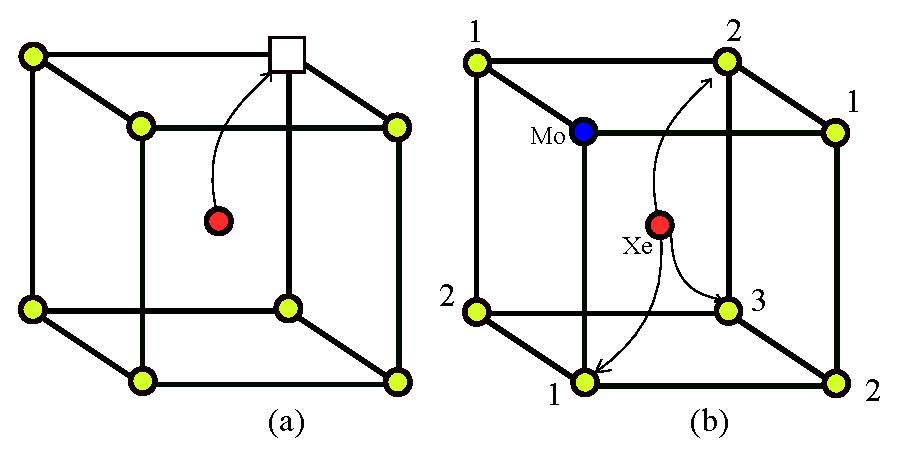
\includegraphics[scale=0.6]{image01}
	\caption{(a)~Diagram of a xenon jump from the centre site to a
    nearest-neighbour vacancy in \textgamma-uranium.
    (a)~All eight jumps are symmetrically equivalent with no molybdenum
    present;
    (b)~with one molybdenum atom in the nearest neighbour shell, there are
        three unique solute jumps (1, 2, and~3).}
      \label{figure01}
\end{figure}

\begin{figure}
    \centering
    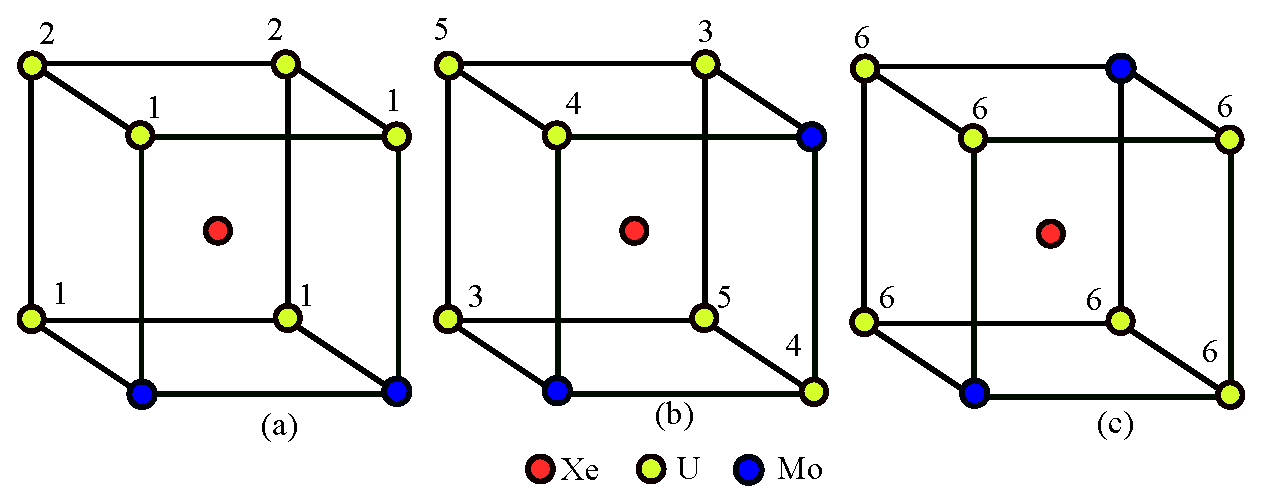
\includegraphics[scale=0.6]{2mo-1xe}
    \caption{The three sets of symmetrically-inequivalent hops of xenon from the centre
        with two molybdenum atoms in the nearest-neighbour shell.
        The numbers denote symmetrically distinct pathways.}
    \label{figure02}
\end{figure}

\begin{figure}
    \centering
    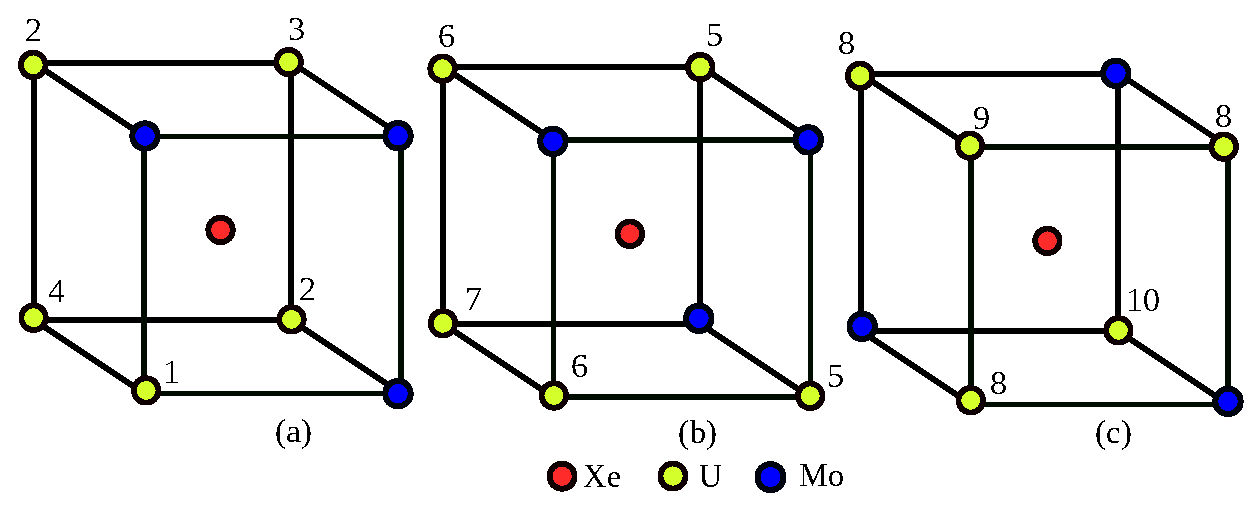
\includegraphics[scale=0.6]{3mo-1xe}
    \caption{The three sets of symmetrically-distinct hops from the centre site
        with three molybdenum atoms in the nearest-neighbour shell. The numbers denote symmetrically distinct pathways.}
    \label{figure03}
\end{figure}

\begin{table}
    \caption{Xenon migration energy ($E_m$) for different configurations.}
    \label{tab_acten}
    \centering
    \begin{minipage}{19.45em}
    \begin{tabular}{ l l l }
      \toprule
        Composition\footnote{The eight nearest-neighbour sites consist of
            one vacancy plus the atoms listed, with the remaining sites
            occupied by uranium atoms.}
        & Xe Jump
        & $E_m$ (eV) \\
      \midrule
        7 U & \hkl<111>~(Fig.~\ref{figure01}a) & 0.161  \\
        1 Mo & 1~(Fig.~\ref{figure01}b) & 0.313 \\ 
             & 2~(Fig.~\ref{figure01}b) & 0.172 \\
             & 3~(Fig.~\ref{figure01}b) & 0.261 \\
        2 Mo & 1~(Fig.~\ref{figure02}a) & 0.110 \\
             & 2~(Fig.~\ref{figure02}a) & 0.212 \\
             & 3~(Fig.~\ref{figure02}b) & 0.532 \\
             & 4~(Fig.~\ref{figure02}b) & 0.108 \\
             & 5~(Fig.~\ref{figure02}b) & 0.224 \\
             & 6~(Fig.~\ref{figure02}c) & 0.110 \\
 	3 Mo & 1~(Fig.~\ref{figure03}a) & 0.515 \\
	     %& 2~(Fig.~\ref{figure03}a) & \tiny{\textcolor{purple}{still running}}		\\
	     & 2$^\prime$~(Fig.~\ref{figure03}a) & 0.917	\\
	     & 3~(Fig.~\ref{figure03}a) & 0.579	\\
	     & 4~(Fig.~\ref{figure03}b) & 0.201	\\
	     & 5~(Fig.~\ref{figure03}b) & 0.384	\\
	     & 6~(Fig.~\ref{figure03}b) & 0.386	\\
	     & 7~(Fig.~\ref{figure03}c) & 1.213	\\
	     & 8~(Fig.~\ref{figure03}c) & 0.461 \\
	     & 9~(Fig.~\ref{figure03}c) & 0.435 \\
      \midrule
             & Mo Jump & $E_m$ (eV) \\% \hline
      \midrule
        7 U & \hkl<111>~(Fig.~\ref{figure01}a)  & 2.067 \\
      \bottomrule
    \end{tabular}
    \end{minipage}
\end{table}



\section{Conclusions}
We calculated solute--vacancy binding energies for different solutes in bcc
uranium. Uranium shows relatively high vacancy--solute binding energies compared to iron and aluminium. The unstable nature of \textgamma-U at low temperature contributes to a significant increase in solute--vacancy binding energy relative to other bcc metals. The higher elastic binding energy in bcc uranium produces a high solute--vacancy binding energy.

We also calculated migration energies of xenon and molybdenum in pure bcc
uranium. Molybdenum's migration energy is very high compared to that of xenon,
indicating that in pure bcc uranium, xenon moves much faster than molybdenum.
The relatively low diffusivity of molybdenum also supports our assumptions that molybdenum is randomly distributed in uranium--molybdenum alloys.
We also studied migration energies of xenon in the presence of molybdenum in
\mbox{U--Mo} alloys.
Different combinations of molybdenum in the nearest neighbour and xenon's
distinct jump paths are identified and studied.
A combinatorial analysis suggests that having up to three molybdenum atoms in
the nearest-neighbour shell is highly probable in U-10Mo and U-7Mo alloys.
The presence of molybdenum in the nearest neighbour shell of a xenon atom has
an impact on the migration energy, but it does not generally increase or
decrease the migration energy; both the location of the molybdenum atoms and
direction of the jump influence the migration energy.
Having one molybdenum atom in the nearest-neighbour shell increases the
activation energy between 0.01~eV and 0.15~eV, depending on the location of
the molybdenum atom relative to the xenon atom and the vacancy.
If xenon has two molybdenum atoms nearby, we found a similar increase,
though there are combinations for which the migration energy is lower than it
is in the single-molybdenum cases.
For xenon with three nearby molybdenum atoms,
the migration energy increases for all molybdenum/\allowbreak{}vacancy
arrangements.
While there are several molybdenum arrangements that result in decreased
migration energies relative to some of the two-molybdenum configurations,
the general trend with the addition of molybdenum in the nearest neighbour
shell near xenon is to increase the migration energy, hence reducing xenon
mobility in \mbox{U--Mo} alloys.
 
We did not consider the influence of molybdenum in the second-nearest neighbour
shell in bcc uranium. Future work should include a determination of diffusion
coefficient of xenon using  the kinetic Monte Carlo method.


%\bibliographystyle{iopart-num}
\bibliographystyle{apsrev4-1}
\bibliography{abbreviated,umox}




\chapter{Helium Impurities and Interaction with Lithium}
\textit{This chapter has been submitted as journal article for peer review. The authors are A. Rafi M. Iasir and Karl D. Hammond of the University of Missouri.}

\section{Introduction}
Lithium is potentially an important element in the context of magnetic fusion
devices. Lithium-coated surfaces have been tested in several fusion devices
around the world~\cite{bell2009plasma, mirnov2003li, sanchez2009impact,
tuccillo2009overview, xu2011study, munaretto2012rfx} and have been found to
increase plasma confinement and improve plasma edge
conditions~\cite{allain2012lithium}.
This behavior is due in part to lithium's ability to trap hydrogen
isotopes~\cite{erents1971trapping}, which has the net result of decreasing
fuel recycling at the plasma edge, leading to higher confinement and fewer
disruptions~\cite{allain2012lithium}.
%Lithium reacts with hydrogen to form lithium hydride (LiH), which is
%ionic in nature.
Lithium has also been proposed as a tritium-breeding material in fusion
reactors~\cite{hartley1978potential} and as a liquid wall-coating ``armor''
to protect plasma-facing components~\cite{Kessel2019}.
%The recent interest in using solid lithium (applied to a graphite or
%tungsten surface) in fusion reactors is for density and impurity control in the
%temperature range of 30--50 \textdegree C~\cite{allain2012lithium}.
In the near-surface region of plasma-facing materials, high densities of
interstitials and vacancies are produced and high concentrations
of hydrogen and helium are present.
These defects and impurities will change the microstructure of the
material~\cite{Hammond2017c}.
It is therefore important to determine the energies of defects in lithium and
their interactions with helium.
This study calculates the energies of several point defects in lithium as
well as the formation, binding, and migration energies of helium atoms and
clusters trapped in lithium. 

\section{Methodology}
We performed all of our calculations using density functional theory (DFT) with
plane-wave basis sets as implemented in the software \textsc{QuantumESPRESSO}~\cite{giannozzi2009quantum}. Projector augmented wave
(PAW)~\cite{blochl1994projector} pseudopotentials from \textsc{QuantumESPRESSO}'s PS library~\cite{dal2014pseudopotentials,pp1} were used.
The density functional of Perdew, Burke, and Ernzerhof (PBE) was used as the
exchange--correlation functional~\cite{Perdew1996b, Perdew1997}. We used a
$4\times4\times4$ supercell of bcc lithium, which consists of 128 atoms, to
simulate defects. Brillouin zone sampling was performed using the scheme of
Monkhorst and Pack~\cite{monkhorst1976special} with a $k$-point mesh of
$5\times5\times5$. The plane wave cutoff energy was 50 Ry. The equilibrium
lattice parameter obtained was 3.436 \AA\@ for bcc lithium. All defect
calculations were performed by fully relaxing the atomic positions in the
supercell at constant volume using this lattice parameter.
The migration energies were calculated using the
nudged elastic band method~\cite{Jonsson1998, henkelman2000climbing,
    henkelman2000improved}
with seven images along the migration pathway.

The formation energies are calculated as follows:
\begin{subequations}
\begin{gather}
 E_{f}^{\text{oct}}  = E_{\text{Li}+\text{He}_{\text{oct}}} - E_{\text{Li}_N} - E_{\text{He}_{\text{isolated}}} \\
 E_{f}^{\text{tetr}} = E_{\text{Li}+\text{He}_{\text{tetr}}} - E_{\text{Li}_N} - E_{\text{He}_{\text{isolated}}} \\
 E_f^{\Box} = E_{\text{Li}_{N-1}} - \frac{N-1}{N} E_{\text{Li}_N} \\
 E_f^{\text{subs}} = E_{\text{Li}+\text{He}_{\Box}} - \frac{N-1}{N} E_{\text{Li}_N} - E_{\text{He}_{\text{isolated}}}.
\end{gather}
 \end{subequations}
Here, $E_{\text{Li}+\text{He}_{\text{tetr/oct}}}$ is the energy of a system in
which helium is situated at either octahedral or tetrahedral sites in bcc
lithium. $E_{\text{Li}+\text{He}_{\Box}}$ is the energy of a system in which
helium is in a substitutional position, $E_{\text{Li}_N}$ is the energy of a
defect-free lithium supercell containing $N$ atoms, and
$E_{\text{He}_{\text{isolated}}}$ is the energy of an isolated helium atom.
$E_{\text{Li}_{N-1}}$ is the energy of a lithium bcc supercell with a lithium
self-vacancy present.

The formation energy of a self-interstitial atom (SIA) is calculated using
\begin{equation}
E_f^{\text{SIA}} = E_{\text{Li}_{N+1}} - \frac{N+1}{N} E_{\text{Li}_N},
\end{equation}
where $E_{\text{Li}_{N+1}}$ is the energy of a system with a lithium
self-interstitial atom starting in either an octahedral or tetrahedral
position. The binding energy of two helium atoms is determined via the formula
\begin{equation}
E_b^{\text{He}_1\text{--}\text{He}_2}
    = E_{\text{Li}_{N}+\text{He}_1} + E_{\text{Li}_{N}+\text{He}_2}
        - E_{\text{Li}_N+\text{He}_1 + \text{He}_2} - E_{\text{Li}_N}.
\end{equation}
Here, $E_{\text{Li}+\text{He}_1}$ is the energy of the supercell with a
single helium interstitial present, and
$E_{\text{Li}_N+\text{He}_1 + \text{He}_2}$
is the energy of the supercell containing two nearby helium atoms in
interstitial positions. For more than two helium atoms, the following equation
is used to calculate the binding energies between them:
\begin{equation}
E_b^{\text{He}_n} = \left (\sum_{i=1}^n E_{\text{Li}_N+\text{He}_i} \right ) - \left[ E_{\text{Li}_N+\text{He}_n} + (n-1)E_{\text{Li}_N} \right].
\end{equation}
The helium--helium dumbbell formation energy (two helium atoms sharing a vacancy) can be calculated using the following equation:
\begin{equation}\label{eq_hedmbl}
  E_f^{\text{He}-\Box-\text{He}}
  = E_{\text{Li}_{N-1}+\text{He}-\Box-\text{He}}
    - \frac{N-1}{N} E_{\text{Li}_N} - E_{\text{He}_{\text{isolated}}}.
\end{equation}
Here, $E_{\text{Li}_{N-1}+\text{He}-\Box-\text{He}}$ is the energy of a supercell containing the helium dumbbell.

\section{Results and Discussion}
We calculated the formation energies for different configurations of the
self-interstitial atoms and the vacancy formation energy for lithium. The
results are presented in Table~\ref{tab:lidmble}. Our results are comparable
with previous DFT calculations and with experiments. Earlier DFT studies
produced formation energies of lithium self-vacancies from 0.52 to
0.57~eV~\cite{benedek1992formation, Pawellek_1991, frank1993properties,
frank1996first}, compared to our value of 0.496~eV\@. The discrepancy could
come from the size of the supercell, elastic interaction, the density
functional, and the quality of the pseudopotential.

We also calculated the self-interstitial formation energy of lithium.
Octahedral self-interstitials are unstable and relax to a dumbbell oriented in
one of the \hkl<100> directions (Fig.~\ref{fig:dmbl}). Tetrahedral
self-interstitials are also unstable and relax to \hkl<110> dumbbells. The
lowest-energy dumbbell orientations are the \hkl<111> orientations, which is a
similar trend as in other non-ferromagnetic bcc materials. The vacancy
formation energy is slightly lower than Frank \etal's value
(0.52~eV)~\cite{frank1996first} and Ma and Dudarev's value
(0.506~eV)~\cite{ma2019effect}, while the migration energy of the vacancy in
\hkl<111> directions is slightly higher than that found by Ma and
Dudarev~\cite{ma2019effect}.
The self-interstitial dumbbell formation energy is comparable to the values
reported by Ma and Dudarev~\cite{ma2019}.

\begin{figure}
	\centering
	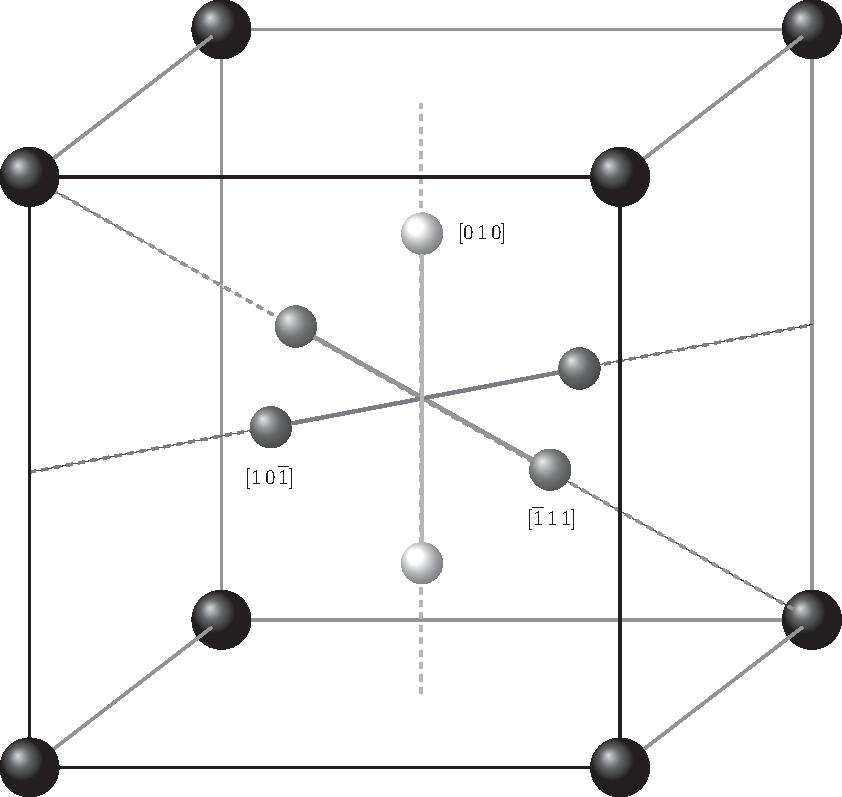
\includegraphics[width=3.3 in]{bcc-dumbbells}
	\caption{Helium--helium dumbbells in different orientations in the bcc
        lithium unit cell.}
	\label{fig:dmbl}
\end{figure}

\begin{table}
\caption[Calculated vacancy formation energy $E_f^{\Box}$, vacancy migration
    energy $E_m^\Box$, and various split-dumbbell and self-interstitial
    formation energies in lithium]{Calculated vacancy formation energy $E_f^{\Box}$, vacancy migration
    energy $E_m^\Box$, and various split-dumbbell and self-interstitial
    formation energies in lithium.
    Results are compared with previous theoretical and experimental results
    (experiments in italics).}
\label{tab:lidmble}
\centering
\renewcommand{\arraystretch}{1.2}
\begin{tabular}{l l l}
  \toprule
  Defect & Energy (eV) & Previous Work \\
  \midrule
  vacancy ($E_f^{\Box}$)
    & 0.496 & 0.506~\cite{ma2019effect} \\
    & & 0.52~\cite{frank1996first} \\
    & & \textit{0.508}~\cite{LandoltBornstein1991} \\
  vacancy ($E_m^\Box$) & 0.086 & 0.053~\cite{ma2019effect} \\ 
    & & \textit{0.038}~\cite{LandoltBornstein1991} \\ 
  \hkl<111> dumbbell ($E_f$) & 0.589 & 0.573~\cite{ma2019} \\
  \hkl<110> dumbbell ($E_f$) & 0.646 & 0.637~\cite{ma2019} \\
  \hkl<100> dumbbell ($E_f$) & 0.791 & 0.782~\cite{ma2019} \\
  tetrahedral ($E_f^{\text{tetr}}$)$^a$ & 0.646 & 0.696~\cite{ma2019} \\
  octahedral ($E_f^{\text{oct}}$)$^b$ & 0.793	& 0.785~\cite{ma2019} \\
  \bottomrule
  \multicolumn{3}{l}{$^a$ equivalent to \hkl<110> dumbbell formation} \\
  \multicolumn{3}{l}{$^b$ equivalent to \hkl<100> dumbbell formation} \\
\end{tabular}
\end{table}


\begin{table}
\caption[Formation energies ($E_f$), binding energies ($E_b$), and migration
  energies ($E_m$, all in eV)
  for helium located at octahedral or tetrahedral interstitial
  sites as well as substitutional sites]{Formation energies ($E_f$), binding energies ($E_b$), and migration
  energies ($E_m$, all in eV)
  for helium located at octahedral or tetrahedral interstitial
  sites as well as substitutional sites. The results are compared with helium
  interactions with tungsten and iron, which are both bcc metals at standard
  temperature and pressure.}
\label{tab:he_li} 
\centering
\renewcommand{\arraystretch}{1.45}
%\begin{minipage}{20.0em}
%\let\footnoterule\relax
\begin{tabular}{l l l l} \toprule
Quantity & Li--He & W--He~\cite{Becquart2006}
    & Fe--He~\cite{seletskaia2005magnetic} \\ \midrule
$E_{f}^{\text{oct}}$        & 1.142 & 6.38 & 4.60 \\
$E_{f}^{\text{tetr}}$       & 1.132 & 6.16 & 4.37 \\
$E_f^{\text{subs}}$         & 1.213 & 4.70 & 4.08 \\
$E^{\ce{T-T}}_m$            & 0.003 & 0.06 & 0.06 \\
$E^{\ce{T-O-T}}_{m}$        & 0.013 & & \\
$E^{\ce{O-O}}_{m}$          & 0.004 & & \\
${E^{\ce{He}-\ce{He}}_b}^a$ & 0.209	& 1.03 & \\ 
${E_b^{\ce{He_s-\Box}}}^b$      & 0.211 \\
${E_b^{\ce{He_t-\Box}}}^c$      & 0.421 \\
	\bottomrule
\multicolumn{4}{p{9 cm}}{$^a$both helium at nearest tetrahedral positions} \\
\multicolumn{4}{p{9 cm}}{$^b$one helium at a substitutional position interacting with
    a vacancy} \\
\multicolumn{4}{p{9 cm}}{$^c$one helium at a tetrahedral position interacting with a
    vacancy} \\
\end{tabular}
%\end{minipage}
\end{table}

\begin{table}
  \caption{Formation energies ($E_f$) of He--He split dumbbells bound to a
    vacancy.}
  \label{tab:hedmble}
  \centering
\renewcommand{\arraystretch}{1.2}
  \begin{tabular}{l l} \toprule
    Orientation & $E_f$ (eV) \\ \midrule
    \hkl<111>   & 1.844 \\
    \hkl<110>   & 1.863  \\
    \hkl<100>   & 1.879 \\ 
  \bottomrule
  \end{tabular}
\end{table}

We now turn our attention to helium interactions with lithium.
During the operation of a plasma device in which lithium is present,
any lithium-coated surfaces will interact with high fluxes of helium and
hydrogen isotopes.
There will also be (n,$\alphaup$) reactions that transmute lithium to
hydrogen and helium. These processes will build up a substantial amount
of hydrogen and helium inside the plasma-facing material. Significant research
has been and is still being performed to understand the behavior of helium in
metals~\cite{Hammond2017c,hammond2020theoretical, samaras2009}. 

One of the major challenges is the low solubility of helium in metals. Helium
atoms in a metal may find low-energy positions either in substitutional or
interstitial lattice sites. We calculated the formation energies of different
configurations of helium in substitutional as well as interstitial positions
in lithium.
The results are presented in Table~\ref{tab:he_li}. We compare our results to
similar configurations in tungsten and iron, two common bcc metals used in
plasma devices. Our calculations predict that the
tetrahedral interstitial position is the lowest-energy interstitial site for
helium, which is also the case for other bcc metals such as tungsten and
iron~\cite{Becquart2006,fu2005}. However, the difference between the octahedral
and tetrahedral interstitial formation energies is only 0.01~eV\@.
This is very low compared to tungsten--helium (0.22~eV~\cite{Becquart2006})
and iron--helium (0.23~eV~\cite{seletskaia2005magnetic})\@.

The formation energy of helium in a substitutional position in lithium is
1.213~eV, which is higher than both the tetrahedral and the octahedral
interstitial formation energies (which are 1.132~eV and 1.142~eV,
respectively).
This is an atypical result compared to helium in other bcc metals or
in fcc metals, for which the substitutional site has a significantly lower
formation energy than the two interstitial
sites~\cite{Becquart2006,seletskaia2005magnetic,Seletskaia2008,Liao2020},
and is more consistent with the energetics of helium in hexagonal close-packed
(hcp) metals~\cite{Yang2011a,Yang2011b}. 
We reproduced this result using a different DFT package
(\ie, \textsc{Abinit}~\cite{Gonze2020,Romero2020})
and got the same values. We also got similar values using ultrasoft
pseudopotentials in \textsc{QuantumESPRESSO}\@.
This is an intriguing result, and will have implications for future simulations
of helium in lithium.

\begin{figure}
	\centering
  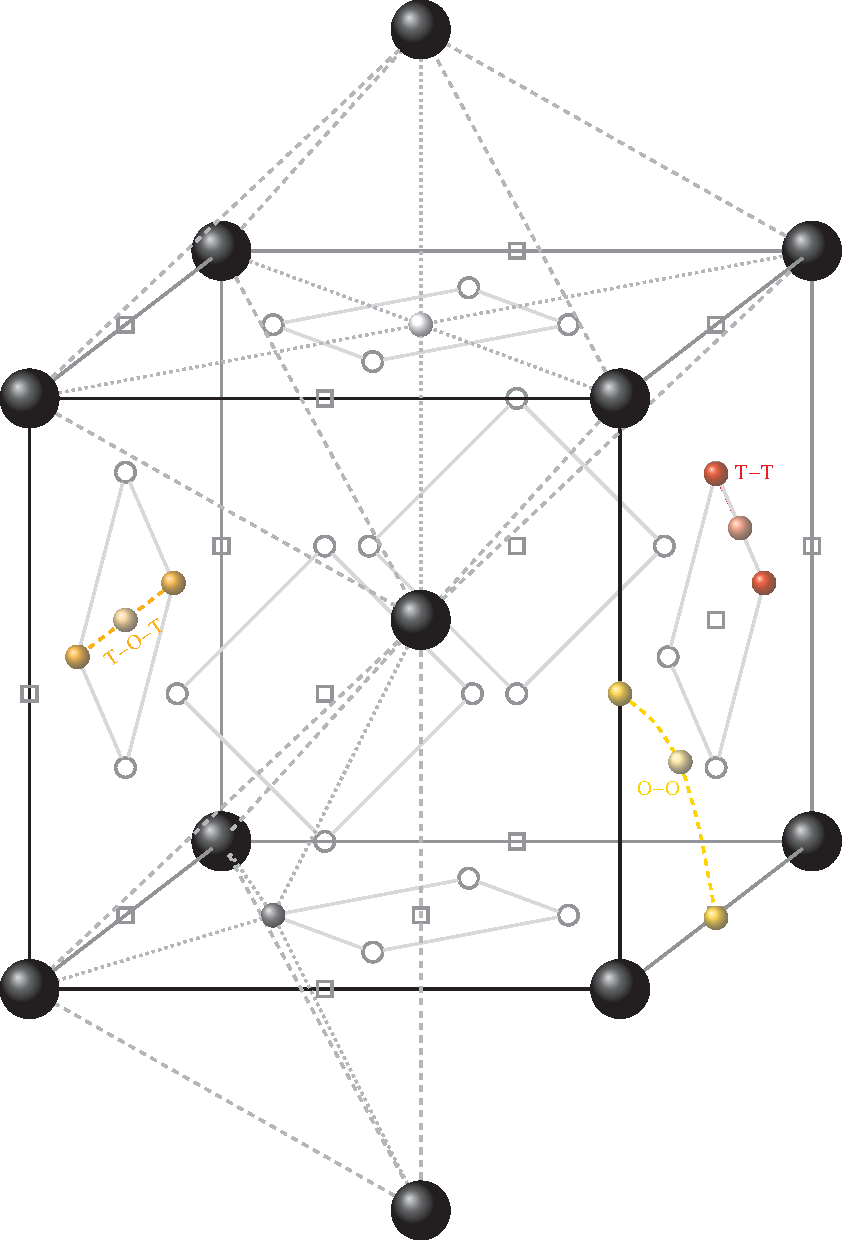
\includegraphics[width=3.9 in]{bcc-sites}
  \caption[Tetrahedral ({\scriptsize$\bigcirc$}) and octahedral ($\square$)
    sites in a bcc crystal]{Tetrahedral ({\scriptsize$\bigcirc$}) and octahedral ($\square$)
    sites in a bcc crystal.
    Three different transition states---tetrahedral to tetrahedral
    (\ce{T-T}), octahedral to octahedral (\ce{O-O}) and tetrahedral to
    octahedral to tetrahedral (\ce{T-O-T})---are shown.}
  \label{fig:tetr}
\end{figure}


Next, we calculated the binding energy of helium to a vacancy.
The substitutional formation energy is higher than the two interstitial
formation energies, though the substitutional site is still the energetic
minimum in the presence of a vacancy.
The binding energy of helium in a substitutional position to a vacancy is
0.21~eV\@.
The binding energy of helium at a tetrahedral interstitial site to a
vacancy is 0.42~eV\@.
The binding energy between two helium atoms at nearby interstitial sites is
0.209~eV, which is lower than that in the tungsten--helium system
(1.03~eV~\cite{Becquart2006}).
The binding energy of multiple helium atoms to a vacancy is also calculated,
and the result is shown in Fig.~\ref{fig:he-bind}. There is a nearly linear
increase in the binding energy as the number of helium atoms increases, which
indicates that a group of helium atoms will tend to aggregate onto a vacancy
and that helium bubble self-nucleation will likely occur in lithium, as it
does in other bcc metals~\cite{Sefta2013b}.


\begin{table}%[htbp]
  \caption{Binding energy of $n$ helium atoms to a vacancy.}
  \centering
  \begin{tabular}{l l}
  \toprule
    $n$ & $E_b$ \\
  \midrule
    %1 & 0.41544262703907636 \\
    %2 & 0.8976585425702422 \\
    %3 & 1.2488173959857483 \\
    %4 & 1.9027688203369273 \\
    %5 & 2.1936052126932073 \\
    %6 & 3.062218788587429 \\
    %7 & 3.2156586866844217 \\
    %8 & 3.9251163930455113 \\
    1 & 0.415\\
    2 & 0.898\\
    3 & 1.249\\
    4 & 1.903\\
    5 & 2.194\\
    6 & 3.062\\
    7 & 3.216\\
    8 & 3.925\\
  \bottomrule
  \end{tabular}
\end{table}


\begin{figure}
  \centering
  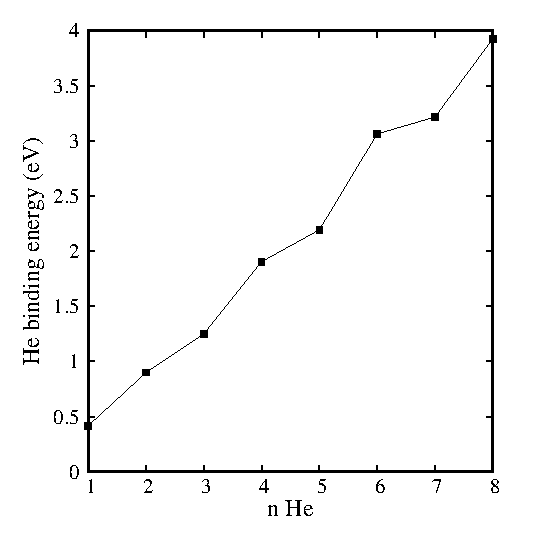
\includegraphics[width=3.8 in]{he-vac-bind-E}
  \caption{Binding energy of $n$ helium atoms to a vacancy for $n \in [1,8]$.}
  \label{fig:he-bind}
\end{figure}

Two helium atoms around a vacancy form a split dumbbell, much like lithium
self-interstitials do. The formation energy varies based on the orientation of
the dumbbell. The helium dumbbell formation energies are presented in
Table~\ref{tab:hedmble}.
The lowest-energy dumbbells have \hkl<111> orientations~(Fig.~\ref{fig:dmbl}).

The migration energies of helium from one tetrahedral site to a nearby tetrahedral site (Fig.~\ref{fig:tetr}) were calculated using the nudged elastic band
method~\cite{Jonsson1998, henkelman2000climbing, henkelman2000improved}.
The migration energy from one tetrahedral site to an adjacent tetrahedral site
(Fig.~\ref{fig:tetr}) is only 0.003~eV, indicating that helium interstitials
will be very mobile in lithium. Helium has a higher migration energy
($E_{m}^{\ce{T-T}}$) in tungsten (0.06~eV~\cite{Becquart2006}) and
iron (0.06~eV~\cite{fu2005}).
The migration energy from one octahedral site to the next octahedral
site ($E_{m}^{\ce{O-O}}$) without passing through a tetrahedral site in lithium
is 0.004~eV, which is also very low.
The low migration energies indicate that helium would be highly mobile in bulk
lithium, much more so than in other bcc metals. It also indicates that bulk
helium diffusion in lithium would be more akin to diffusion in gases or
liquids, with a $T^{3/2}$ dependence of the diffusion coefficient arising from
translational motion, but without the Arrhenius temperature dependence
associated with vibrational motion. This result, combined with the higher
formation energy of substitutional helium compared to interstitial helium,
suggests that helium transport in lithium will be fundamentally different than
it is in iron, nickel, tungsten, and other metals.

\nomenclature{$E_f^{\text{subs}}$}{helium formation energy in a substitutional position}
\nomenclature{$E_f^{\text{tetr}}$}{helium formation energy in a tetrahedral position}
\nomenclature{$E_f^{\text{oct}}$}{helium formation energy in a octahedral position}
\nomenclature{$E_{\text{He}_{\text{isolated}}}$}{energy of an isolated helium atom}
\nomenclature{$E_f^{\text{He}-\Box-\text{He}}$}{helium--helium dumbbell formation energy around a vacancy}
\nomenclature{$E_b$}{binding energy}

\clearpage
\bibliographystyle{apsrev4-2}
\bibliography{abbreviated,final}



\chapter{Conclusions and Future Work}
We have studied the impact of fission gas in U--Mo alloy. The distributed xenon and krypton gas inside the fuel has significant impact on the thermal properties on the fuel. Krypton is also a fission products which constitutes almost 10\% of the fission gas. In comparison to pure xenon bubbles in U--10Mo, their mixture has very little differences. This reaffirms that, xenon contributes the most in the reduction of thermal conductivity. Both intra- and inter-granular xenon bubbles impacts on the heat transfer. The arrangements of the bubbles inside the fuel has significant impact the direction of the heat transfer.





\bibliography{abbreviated,comp}






\appendix
\chapter{Atomic Units}\label{appen_atomicunit}
There are special units of measurement which is convenient for atomic physics and DFT calculations. They are named after the Physicist Douglas Hatree~\cite{hartree}. In this system the numerical values of the four fundamental physical constants are assumed to be unity. They are as follows:
\begin{itemize}
\item Reduced planck constant: $\hbar = 1$, atomic unit of action.
\item Elementary Charge: $e = 1$, atomic unit of charge.
\item Bohr radius: $a_0 = 1$, atomic unit of length.
\item Electronic mass: $m_e = 1$, atomic unit of mass.
\end{itemize}
Now we will explore how it simplifies quantum mechanical calculation of hydrogen atom. The hydrogen atom consists of a heavy proton (charge $e$) with a much lighter electron (charge $-e$) that orbits around it. The potential energy (in SI units) is
\begin{equation}\label{eq_hyd_pot}
V(\vb{r}) = -\frac{Ze^2}{4\pi \epsilon_0 \abs{r}}
\end{equation}
where $Z$ is the atomic number and $\vb{r}$ is the position relative to the nuclear site. The radial Schr\"odinger equation including the centrifugal term is:
\begin{equation}\label{eq_hdr_atom}
	\left [ -\frac{\hbar^2}{2m_e}\nabla_r^2 + \frac{\hbar^2 \ell (\ell+1)}{2m_er^2} - \frac{Ze^2}{4\pi \epsilon_0 \abs{r}} - E \right ]rR(r) = 0
\end{equation}
The above equation can be simplified by introducing dimensionless quantities. Multiplying Eq.~\eqref{eq_hdr_atom} with $m_e/\hbar^2$ the equation becomes:
\begin{align}
\begin{split}
\left [-\nabla^2_r + \frac{\ell(\ell+1)}{r^2} + \frac{2m_eZe^2}{4\pi\epsilon_0\hbar^2} \frac{1}{r} - \frac{2m_eE}{\hbar^2} \right ] rR(r) & = 0 \\
\left [ -\frac{1}{2} \nabla_r^2 + \frac{\ell(\ell+1)}{2r^2} + \frac{Z}{a_0r} - \frac{E}{E_0a_0^2}    \right ]rR(r) & = 0 \\
\left [-\frac{1}{2}\nabla_{\zeta}^2 + \frac{\ell(\ell+1)}{2\zeta^2} + \frac{Z}{\zeta} - \frac{E}{E_0}    \right ] \zeta R(\zeta a_0) & = 0
\end{split}
\end{align} 
The above equation has two units, one is for length scale, the Bohr radius $a_0$ and the other one is an energy scale, the Hartree $E_0$.
\subsection{Bohr Radius}
\begin{equation}
\label{eq_bohr}
a_0 = \frac{4\pi\epsilon_0 \hbar^2}{m_ee^2}
\end{equation}
The Bohr radius is the length unit of the Hatree atomic unit system. It corresponds to the radius of a classical electron circling a proton at the ground energy of the hydrogen atom. Using all the fundamental constants in Eq.~\eqref{eq_bohr} the standard atomic unit of Bohr becomes
\begin{equation}
1\ \text{bohr} = \frac{4\pi\epsilon_0 \hbar^2}{m_ee^2} = \num{0.52917725e-10} \text{m} = 0.52917725 \ \AA
\end{equation}


\subsection{Hatree}
\begin{equation}
\label{eq_htr}
 E_0= \frac{\hbar^2}{m_ea_0^2} = \frac{m_ee^4}{(4\pi\epsilon_0\hbar)^2}
\end{equation}
The Hartree is the energy unit in the Hatree atomic unit system. One Hartree is twice the binding energy of an electron in the hydrogen atom. To satisfy $a_0 = 1$, all the fundamental units becomes unity ($\hbar = m_e = e = 4\pi\epsilon_0 = 1$), according to Eq.~\eqref{eq_bohr}. The unit of Hatree can also be calculated from the fundamental units.
\begin{equation}
1\ \text{hartree} = \frac{\hbar^2}{m_ea_0^2} = \frac{m_ee^4}{(4\pi\epsilon_0\hbar)^2} = \num{4.3597482e-10} \text{J} = 27.211396 \  \text{eV}
\end{equation}

In Hatree units, the Schr\"odinger equation of an electron in the Coulomb potential of the nucleus has the following form:
\begin{equation}
\left(-\frac{1}{2}\nabla^2 - \frac{Z}{r} - E \right) \ket{\psi} = 0
\end{equation}

\subsection{Rydberg Atomic Units}
The Rydberg atomic unit is another useful atomic unit which is widely used in DFT and atomic physics. In Hatree atomic units, the assumption is $\hbar^2/2m_e = \frac{1}{2}$. In Rydberg atomic units the assumption is: 
\begin{equation*}
\hbar = 2m_e = e^2/2 = 1
\end{equation*}
Using the above relations, the length unit does not change in Rydberg units.
\begin{equation}
a_0 = \frac{4\pi\epsilon_0 \hbar^2}{2m_ee^2/2} = \frac{4\pi\epsilon_0 \hbar^2}{m_ee^2} = 0.52917725 \ \AA
\end{equation}

The energy unit does change as follows:
\begin{equation}
1\ \text{Ry} =  \frac{\hbar^2}{2m_ea_0^2} = \frac{1}{2} \frac{\hbar^2}{m_ea_0^2} = 13.605693\  \text{eV}
\end{equation}








\bibliography{abbreviated,comp}
\bibliographystyle{iopart-num}

%\chapter{Helium Interaction with BCC Lithium}
Lithium is becoming one of the important materials in the context of plasma-facing in thermonuclear magnetic fusion devices. Lithium-coated surfaces are being used in several fusion devices in the world~\cite{bell2009plasma, mirnov2003li, sanchez2009impact, tuccillo2009overview, xu2011study, munaretto2012rfx}. There are earlier example of using lithium in the fusion reactor. Erents \etal~\cite{erents1971trapping}\@ used lithium to trap deutorons in solid and liquid lithium. Liquid lithium proven to be efficient trapper. Lithium reacts with deuterium and forms lithium hydride (LiH) which is ionic in nature. Lithium was also proposed as a breeding material in fusion reactors~\cite{hartley1978potential}. For this, lithium needs to be enriched to $^6$Li. The recent interest of using solid lithium (applied to graphite surface) in fusion reactor is for density and impurity control in the temperature range of 30--50 \textdegree C~\cite{allain2012lithium}.  In the near surface of plasma facing materials high density of interstitials and vacancies are being produced in addition to higher concentration of hydrogen and helium. This defects and gases will change the microstructure of the material. It is therefore important to determine the property of point defects in Lithium and its interaction with helium atom. The goal of this study is to calculate some important data regarding point defects in lithium and helium in lithium using first principle methods.

We perform all our calculations using density functional theory (DFT) with plane-wave basis sets as implemented in the software \textsc{QuantumEspresso}\cite{giannozzi2009quantum}. The PAW~\cite{blochl1994projector} based pseudopotential were used from PS library~\cite{dal2014pseudopotentials,pp1}. The generalized gradient approximation of Perdew--Burke--Ernzerhof (PBE) was used as exchange-correlation functional~\cite{Perdew1996b, Perdew1997}. We used a $4\times4\times4$ of bcc lithium, which consists of 128 atoms to simulate point defects. Brillouin zone sampling was performed using Monkhorst and Pack scheme~\cite{pack1977special}. The plane wave cutoff energy was 50 Ry. The equilibrium lattice parameter obtained was 3.436 \AA\@ for bcc lithium. All the calculations were performed at constant volume fully relaxing the atomic positions in the supercells. The migration energies were calculated using the nudged elastic band~\cite{henkelman2000climbing, henkelman2000improved} method with five images along the migration path.

The formation energies are calculated as follows:
\begin{align}\label{eq_forme}
\begin{split}
 E_{f}^{\text{oct}} & = E_{\text{Li}+\text{He}_{\text{oct}}} - E_{\text{Li}_N} - E_{\text{He}_{\text{isolated}}} \\
 E_{f}^{\text{tetr}}& = E_{\text{Li}+\text{He}_{\text{tetr}}} - E_{\text{Li}_N} - E_{\text{He}_{\text{isolated}}} \\
 E_f^{\Box} & = E^{{\Box}_1}_{\text{Li}_{N-1}} - \frac{N-1}{N} E_{\text{Li}_N} \\
 E_f^{\text{subs}} & = E_{\text{Li}+\text{He}_{\Box}} - \frac{N-1}{N} E_{\text{Li}_N} - E_{\text{He}_{\text{isolated}}}
\end{split}
 \end{align}

\nomenclature{$E_f^{\text{subs}}$}{helium formation energy in a substitutional position}
\nomenclature{$E_f^{\text{tetr}}$}{helium formation energy in a tetrahedral position}
\nomenclature{$E_f^{\text{oct}}$}{helium formation energy in a octahedral position}
\nomenclature{$E_{\text{He}_{\text{isolated}}}$}{energy of an isolated helium atom}



Here $E_{\text{Li}+\text{He}_{\text{tetra/octa}}}$ is the energy of the system where He is in either octahedral and tetrahedral location of bcc lithium. $E_{\text{Li}+\text{He}_{\Box}}$ is the energy of the system where He is in substitutional position of the lattice. $E_{\text{Li}_N}$ is the reference energy of the bulk bcc lithium, and $E_{\text{He}_{\text{isolated}}}$ is the energy of an isolated He atom. $E^{\Box_1}_{\text{Li}_{N-1}}$ is the energy of a lithium bcc supercell with a vacancy.


The formation energy of an SIA is calculated using
\begin{equation}
E_f^{\text{SIA}} = E_{\text{Li}_{N+1}}^{\text{SIA}} - \frac{N+1}{N} E_{\text{Li}_N}
\end{equation}
where, $E^{\text{SIA}}_{\text{Li}_{N+1}}$ is the energy of a system with a self interstitial (Li) atom in in either octahedral and tetrahedral position.


The binding energies of two helium atoms is determined as obtained as: 
\begin{equation}
E_{\text{b}}^{A_1\text{--}A_2} = E_{\text{Li}}^{A_1} + E_{\text{Li}}^{A_2} - E_{\text{Li}_N}^{A_1+A_2} - E_{\text{Li}_N} 
\end{equation}

\begin{table}
\caption[Defect formation energies in bcc lithium]{Calculated vacancy formation energy $E_f^{\Box}$, vacancy migration energy, and self-interstitial formation energy in lithium. Calculated results are compared with some of the previous work and experimental results (in italics).}
\label{tab:lidmble}
\centering
\begin{minipage}{28.5em}
\let\footnoterule\relax
\begin{tabular}{c c c} \toprule
Defect					& Formation Energy (eV)						& Previous Work \\ \midrule
						&											& 0.52~\cite{frank1996first} \\ 
vacancy ($E_f^{\Box}$)	& 0.496										& 0.506~\cite{ma2019effect} \\
						&										& \textit{0.508}~\cite{LandoltBornstein1991} \\ \hline
\hkl<111>			   & 0.589										&  0.573~\cite{ma2019}	 \\ \hline
\hkl<110>\footnote{equivalent to tetrahedral SIA formation}   & 0.646 & 0.637~\cite{ma2019}	 \\ \hline
\hkl<010>\footnote{equivalent to octahedral SIA formation}   & 0.791 &  0.782~\cite{ma2019}    \\ \hline
tetrahedral ($E_f^{\text{tetr}}$) &	0.646 &	0.696~\cite{ma2019}	\\ \hline
octahedral ($E_f^{\text{oct}}$) & 0.793	& 0.785~\cite{ma2019}	\\ \hline
Vacancy migration energy       & 0.102 & 0.053~\cite{ma2019effect}	\\ 
							   &       & \textit{0.038}~\cite{LandoltBornstein1991} \\ 
\bottomrule
\end{tabular}
\end{minipage}
\end{table}


Here, $E_{\text{Li}_N}$ is the energy of the supercell without any $A_1$ and $A_2$, $E^{A_1/A_2}_{\text{Li}}$ is the energy of the supercell with $A_1$ or $A_2$. $E_{\text{Li}}^{A_1+A_2}$ is the energy of the supercell containing both $A_1$ and $A_2$ interacting.  For more than two entities, the following equation is used to calculate the binding energies between them.
\begin{equation}
E_b^{(A_1,A_2,\dots,A_n)} = \sum_{i=1,\dots,n} E^{A_i}_{\text{Li}} - \left[ E^{(A_1 + A_2 + \dots + A_n)}_{\text{Li}} + (n-1)E_{\text{Li}_N} \right ]
\end{equation}


The He--He dumbbell formation energy (around a vacancy) can be calculated using the following equation:
\begin{equation}\label{eq_hedmbl}
E_f^{\text{He}-\Box-\text{He}} = E_{\text{Li}}^{\text{He}-\Box-\text{He}} - E_{\text{Li}_N} + \frac{E_{\text{Li}_N}}{N} - E_{\text{He}_{\text{isolated}}}
\end{equation}

\nomenclature{$E_f^{\text{He}-\Box-\text{He}}$}{helium--helium dumbbell formation energy around a vacancy}

Here, $E_{\text{Li}}^{\text{He}-\Box-\text{He}}$ is the energy of the system containing helium dumbbell.

We have calculated the formation energies for different configurations of the self-interstitial atom and the vacancy formation energy for lithium. The results are presented in Table~\ref{tab:lidmble}. Our results are compatible with previous DFT works and experiments. The earlier DFT works produced formation energies range from 0.52--0.57 eV~\cite{benedek1992formation, Pawellek_1991, frank1993properties, frank1996first}. The discrepancy could come from the size of the supercell (54), elastic interaction and the quality of the pseudopotential. We have also calculated the self-interstitial formation energy in lithium. The octahedral self-interstitial forms a dumbbell in \hkl<010> direction, and the tetrahedral interstitial forms a \hkl<110> dumbbell. The most stable dumbbell being in the direction of \hkl<111>, which is very similar to other nonmagnetic bcc materials. The vacancy formation energy is slightly underestimated while the migration energy of the vacancy in \hkl<111> direction is  over estimated. The self-interstitial dumbbell formation shows similar comparable values as reported by Ma and Dudarev~\cite{ma2019}.


\begin{table}
\caption[Formation energy of helium in lithium]{Formation energies (in eV) for a single He atom positioned in the octahedral or tetrahedral interstitial sites as well as in substitution. He migration energy (eV). The Calculations are done using 128 atom supercells.}
\label{tab:he_li} 
\centering
\begin{tabular}{c c c c} \toprule
Configuration   & Li--He  &  W--He~\cite{becquart2007ab}   &  Fe--He~\cite{seletskaia2005magnetic} \\ \midrule
    $E^{f}_{\text{oct}}$  & 1.142   &  6.38    & 4.60   \\ \hline
    $E^{f}_{\text{tetr}}$ & 1.132   &  6.16    & 4.37   \\ \hline
    $E^f_{\text{subs}}$          & 1.213   &  4.70    & 4.08   \\ \hline
    $E^{t-t}_{\text{mig}}$       & 0.003   &  0.06    & 0.06    \\ \hline 
	$E^{t-o-t}_{\text{mig}}$     & 0.013   &		   &		\\ \hline
	$E^{o-o}_{\text{mig}}$		  & 0.004   &			&		\\ \hline
    $E^{\text{He}-\text{He}}_b$   & 	    &  1.03		 &		\\ 
	\bottomrule
\end{tabular}
\end{table}

\begin{table}
\caption[He--He dummbbell formation energy in lithium]{Formation of  He--He dumbbells around a vacancy}
\label{tab:hedmble}
\centering
\begin{tabular}{c c} \toprule
Dumbbell Configuration & Formation Energy (eV) \\ \midrule
\hkl<111>   & 1.844 \\ \hline
\hkl<110>   & 1.863  \\ \hline
\hkl<010>   & 1.879 \\ 
\bottomrule
\end{tabular}
\end{table}

During the operation of the fusion reactor, the lithium coated surface will be interacting with high flux of different hydrogen isotopes and helium plasmas. This could initiate neutron activated reaction and transmute hydrogen and helium. All these processes will build a substantial amount of hydrogen and helium inside the material. Numerous research has been and still being performed to understand the behaviour of helium in metals. One of the major challenges is the low solubility of helium in metal. Helium atoms in a metal may find its low energy position either in substitutional or interstitial lattice sites. We have calculated the formation energies of different configuration of helium in substitutional as well as interstitial positions using Eq.~\eqref{eq_forme}. The results are presented in Table~\ref{tab:he_li}. We have compared our results with tungsten and iron's interaction with helium. Our calculation predicts that, tetrahedral interstitial position is the most stable configuration for helium, which is also common for tungsten and iron~\cite{becquart2007ab,fu2005}. The difference between the octahedral and tetrahedral interstitial formation energy is 0.01 eV. This is low compared to tungsten--helium (0.22 eV) and iron--helium (0.23 eV). The formation energy of helium in a substitutional location is about 1.213 eV. This value is higher than both tetrahedral and octahedral interstitial formation energy. This is an atypical result compared to tungsten--helium and iron--helium system. We have reproduced our results of having higher substitutional energy using different DFT package (\ie\@ Abinit) and ultrasoft pseudopotential. 

We have also calculated the binding energy of helium with monovacancy. Even though, the substitutional energy is higher, a single helium still finds its place in lattice side. The binding energy of a helium in lattice site with a nearby vacancy is 0.21 eV. The binding energy of a helium in tetrahedral interstitial location and nearest vacancy is 0.42 eV. This indicates that a interstitial helium favors the vacancy. Two helium atoms around a vacancy forms dumbbell. The formation energies are based on the orientation of the dumbbell. The helium dumbbell formation energies are presented in Table~\ref{tab:hedmble}. The lowest energy configuration is \hkl<111> dumbbell. The migration energies of helium from one tetrahedral site to nearest tetrahedral site (Fig.~\ref{fig:001}) is calculated using nudged elastic band method. The calculated energy is 0.003 eV. Tungsten--helium and iron--helium have a little higher migration ($E_{mig}^{t-t}$) energy of 0.006 eV. The migration energy from one octahedral site to the next octahedral site is 0.004, which is also very low.



\begin{figure}
\centering
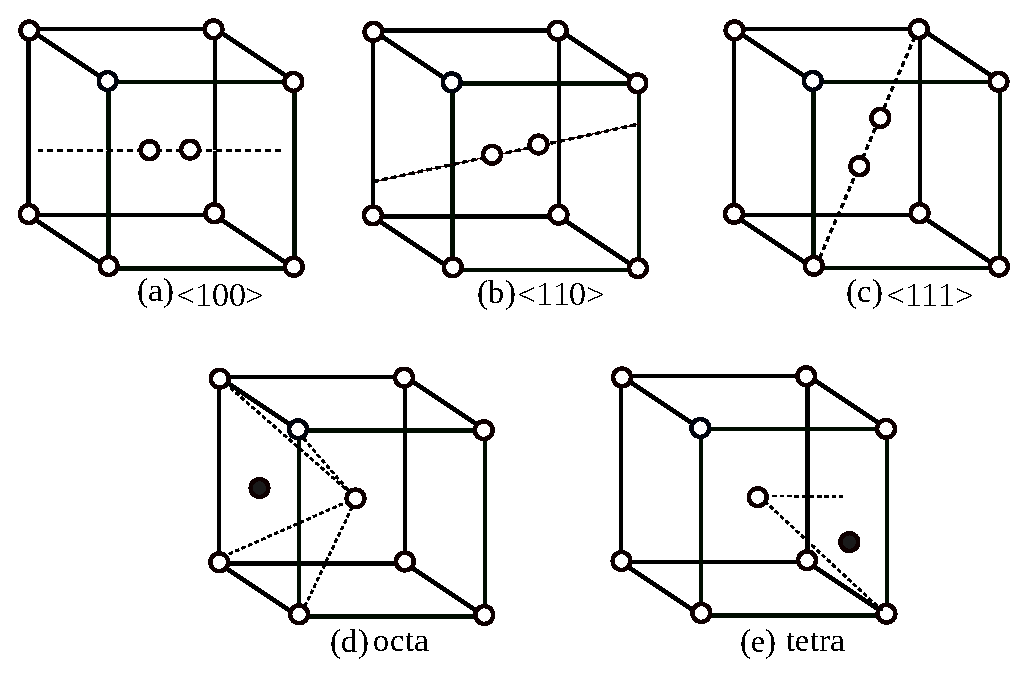
\includegraphics[scale=0.7]{dumbl_figs}
\caption[Different dumbbell configuration in bcc lithium]{Different dumbbell configuration in bcc crystal. a) \hkl<100> dumbbell. b) \hkl<110> dumbbell. c) \hkl<111> dumbbell. d) octahedral interstitial. e) tetrahedral interstitial.}
\label{fig:dmbl}
\end{figure}

\begin{figure}
\centering
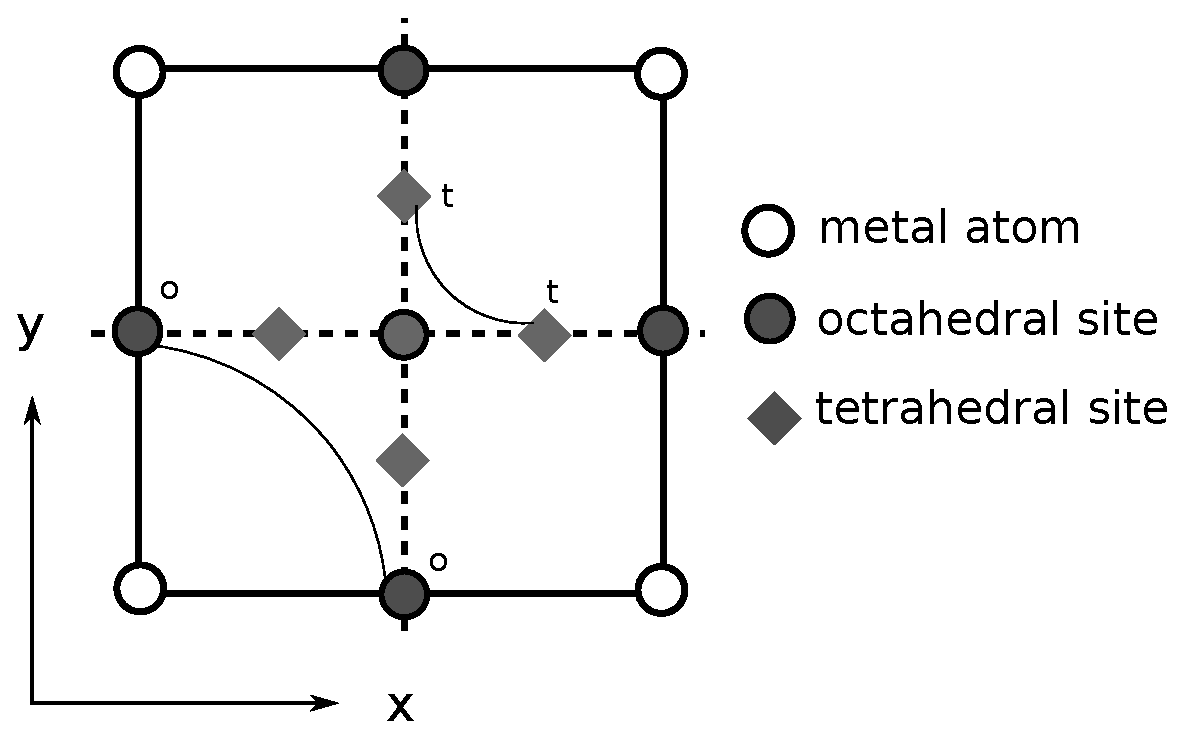
\includegraphics[scale=0.6]{001_oct_tetra}
\caption[Interstitial atom location in 2D for bcc crystal]{Tetrahedral (t) and octahedral (o) site on the (001) plane of the bcc lattice.}
\label{fig:001}
\end{figure}

\begin{figure}
\centering
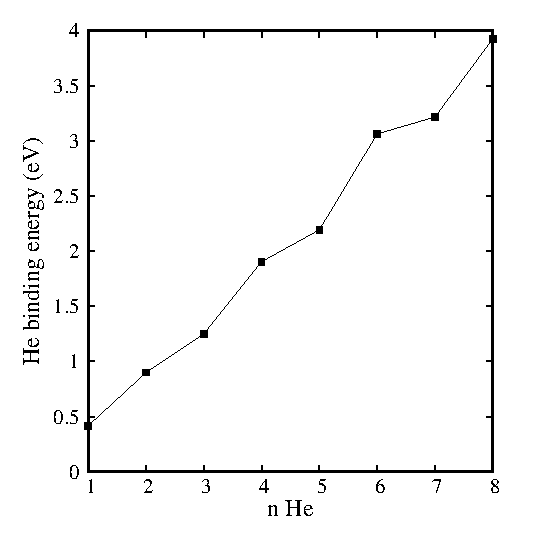
\includegraphics[scale=1.2]{he-vac-bind-E}
\caption[He binding energy]{Helium binding energy around a vacancy}
\label{fig:he-bind}
\end{figure}

\pagebreak
%\bibliographystyle{iopart-num}
\bibliographystyle{apsrev4-1}
\bibliography{abbreviated,lihe}

\chapter{Orthogonal Plane Wave}\label{appen_opw}

For now we will try to approximate time-independent \schrod equation so that we can achieve self-consistency. We let $V(r)$ the potential seen by each electron. Then each energy eigenfunction will satisfy the following equation:
\begin{equation}
\label{eigeqn}
H\psi_i = (T+V(r))\psi_i = E_i\psi_i 
\end{equation}
Here $T$ is the kinetic energy ($-\hbar^2\nabla^2/2m$), and $E_i$ is the energy of the ith state. The next step is to distinguish between the core and the valance state. The index $\alpha$ will be used for core and $v$ will be used for conduction band. According to our second assumption, the core states are the same as in the isolated ion, but their energies are different, i.e. $E_\alpha$, are different:
\begin{equation}
\label{eq_eigalpha}
(T+V(r))\psi_\alpha = E_\alpha \psi_\alpha
\end{equation}
Here, the subscript $\alpha$ not only denotes the position of the ion as well as the energy and angular-momentum quantum numbers of the state in the equation. We have an well defined eigen value problem, apart from not knowing $V(r)$. We can approach the problem in several ways. The choice of basis function is often used physics. The plane wave basis sets is often used in band structure calculations. If we expand the \schrod equation \ref{eq_eigalpha} with complete set of states,  then we may obtain a linear simultaneous equations in the expansion coefficients. The problem of  solving differential equations become a matrix diagonilizing problem. The choice of plane waves has its pros and cons. One of the difficulties of using plane waves, is that, it requires a large number of plane waves to give a reasonable description of the wave function. Thus the solution becomes very difficult. Core electron has higher kinetic energy (s orbital) near the nucleus (see Fig.~\ref{fig_hydrogen}), which makes it really hard for plane wave to approximate those oscillation. Herring~\cite{herring1940new} suggested that, rather than expanding the conduction electron wave function in plane waves, a more rapidly convergent procedure is to expand in \textit{orthogonalized} plane waves (OPWs). Hopefully, the expansions in terms of OPWs, would require fewer terms and therefore yield a easier calculation. The OPWs with wave number $\mathbf{k}$ can be defined as follows:
\begin{equation}
\label{eq_opw}
OPW_{\vb{k}} = e^{i\vb{k.r}} - \sum_{\alpha} \psi_{\alpha}(\vb{r}) \psi^{\ast}_{\alpha} e^{i{\vb{k.r}}} d\tau'
\end{equation}

An example would be sodium, where it has a ground state configuration of $1s^2 2s^2 2p^6 3s^1$, the core level would represent $1s^2 2s^2 2p^6$. For so-called simple metal (i.e. Na, Mg and Al), the convergent electron wave function is rapidly convergent in the OPW basis. Before going any further, lets check whether this OPW (\ref{eq_opw}) is orthogonal to the core states. Lets assume an arbitrary core wave function $\psi_{\beta}$ and check the orthogonality with \ref{eq_opw}.
\begin{equation}
\int\psi^{\ast}_{\beta}(\vb{r})OPW_{\vb{k}}d\tau' = \int \psi^{\ast} (\vb{r}) e^{i\vb{k.r}} d\tau - \sum_{\alpha} \delta_{\alpha\beta} \int \psi^{\ast} (\vb{r'}) e^{i\vb{k.r'}} d\tau' = 0 
\end{equation}
It is convenient to normalize the plane waves in the unit cell volume of the metal $\Omega$, and we will bra and ket notation for the wave functions from now on. The plane wave becomes
\begin{equation}
	\ket{\vb{k}} \equiv \Omega^{-1/2}e^{i\vb{k.r}}
\end{equation}
For core electron wave functions
\begin{equation}
	\ket{\alpha} \equiv \psi_{\alpha} (\vb{r}) 
\end{equation}
where a bra operators is defined as $\bra{\alpha} = \ket{\alpha}^{\ast}$, the other representation an integral:
\begin{equation}
	\braket{\alpha}{\vb{k}} = \Omega^{-1/2} \int \psi^{\ast}_{\alpha} (\vb{r}) e^{i\vb{k.r}}
\end{equation}
Thus the OPW equations becomes
\begin{equation}
	OPW_{\vb{k}} = \ket{\vb{k}} - \sum_{\alpha} \ket{\alpha}\braket{\alpha}{\vb{k}}
\end{equation}
The projection operator $P$ can be defined as follows:
\begin{equation}
\label{eq_proj}
P = \sum_{\alpha} \dyad{\alpha}{\alpha}
\end{equation}
The $P$ operator projects any function onto core states. In terms of $P$ operator the OPW can take following form
\begin{equation}
	OPW_{\vb{k}} = (1-P)\ket{\vb{k}}
\end{equation}
Now, we can expand the conduction-band (valence electron) state in terms of the general linear combination of  OPW's:
\begin{equation}
	\psi_{k} = \sum_q a_q (\vb{k})(1-P)\ket{\vb{k}+\vb{q}}
\end{equation}
Before going a bit further, lets see how kinetic energy is represented by planewaves.
\begin{equation}
\label{eq_kin}
	\bra{q'}-\frac{\hbar^2}{2m}\nabla^2\ket{q} = \frac{1}{2}\frac{\hbar^2}{2m} \abs{\vec{q}}^2 \delta_{\vec{q}\vec{q}'}
\end{equation}
In the above approximation of kinetic energy we assumed the normalizing factor is one.
Now we are going to expand \ref{eq_eigalpha} with OPWs, and the \schrod equation becomes
\begin{equation}
H\psi_k = \sum_q a_q (\vb{k})H(1-P)\ket{\vb{k}+\vb{q}}=E_k\sum_q a_q (\vb{k}) (1-P) \ket{\vb{k}+\vb{q}}
\end{equation}
Where , $H$ consists both the kinetic energy and the potential. Multiplying on the left by $\bra{\vb{k}+\vb{q}'}$, and using Equation~\eqref{eq_kin} we obtain
\begin{multline}
\label{eq_opwd}
a_{q'} (\vb{k}) \frac{\hbar^2}{2m}\abs{\vb{k}+\vb{q}'}^2 + \sum_q a_q (\vb{k}) \\
	\times
[\bra{\vb{k}+\vb{q}'}V\ket{\vb{k}+\vb{q}} - \sum_{\alpha} E_{\alpha} \braket{\vb{k}+\vb{q}'}{\alpha}\braket{\alpha}{\vb{k}+\vb{q}}]
	= [a_{q'} (\vb{k}) - \sum_q a_q (\vb{k}) \bra{\vb{k}+\vb{q}'}P\ket{\vb{k}+\vb{q}}]E_{\vb{k}}  
\end{multline}
The above equation can be solve by diagonalizing some of matrix element. If we can evaluate some of the various matrix elements (integrals), we obtain a set of linear algebraic equation.


\bibliographystyle{unsrt}
\bibliography{abbreviated,comp}
%\bibliographystyle{unsrt}
%\bibliography{abbreviated,comp}


\chapter{Projector Augmented Wave}\label{appen_paw}

The pseudopotential technique has proven to be accurate for a large variety of systems, but there is no strict guarantee that it will produce the same results as an all-electron calculation. The challenge with norm-conserving pseudopotentials is that they limit the \textit{softness}. Another way to say it is that, it requires a high cut-off energy. In the plane-wave basis set for the pseudo wavefunctions is defined by the shortest wave length $\lambda=2\pi/\abs{\vb{G}}$, where $\vb{G}$ is the wave vector. Projector augmented waves (PAW) introduces projectors and auxiliary localized functions to increase the softness of the pseudopotential, while at the same time keeping the full wavefunction. In this section, I will try to introduce PAW with basic formalism. The origin of the PAW method lies in a transformation that maps the true wavefunctions with their complete nodal structure onto auxiliary wavefunctions. The purpose of this transformation is to have smooth auxiliary wavefunctions that have a rapidly convergent plane-wave expansion. The PAW method was first proposed by Bl\"ochl in 1994~\cite{blochl1994projector}. The linear transformation is as follows:
\begin{equation}
\ket{\Psi_n} = \hat{\mathcal{T}}\ket{\tilde{\Psi}_n}
\end{equation}
where, $\ket{\Psi_n}$ is the true all-electron Kohn--Sham (KS) single-particle wavefunction, $\ket{\tilde{\Psi}_n}$ is an auxiliary smooth wavefunction, and $\hat{\mathcal{T}}$ is a linear transformation operator. Since the true wavefunctions are already smooth at a certain minimum distance from the core, $\tilde{\mathcal{T}}$ should only modify the wavefunction close to the nuclei. Thus the transformation operator becomes
\begin{equation}
\tilde{\mathcal{T}} = 1 + \sum_a \tilde{\mathcal{T}^a},
\end{equation}
where $a$ is an atom index and $\tilde{\mathcal{T}^a}$ has no effect outside a certain atom-specific augmentation region, $r_C^a$. Inside the augmentation spheres, the true wavefunction can be expanded in the partial waves $\phi_i^a$, for a corresponding auxiliary smooth partial wave can be defined as $\tilde{\phi}_i^a$, and they can be connected by the following relation:
\begin{equation}
\label{eq_aug_t}
\ket{\phi_i^a} = (1+\hat{\mathcal{T}}^a)\ket{\tilde{\phi}_i^a} \Rightarrow  \hat{\mathcal{T}}^a \ket{\phi_i^a} = \ket{\phi_i^a} - \ket{\tilde{\phi}_i^a}.
\end{equation} 
Here $a$ is an atom index and $i$ denotes partial waves. Outside the augmentation sphere, the partial wave and its smooth counterpart should be identical:
\begin{equation}
\phi_i^a(\mathbf{r}) = \tilde{\phi}_i^a(\mathbf{r})\quad \text{for} \quad r > r_c^a
\end{equation} 
Where $\phi_i^a(\mathbf{r})=\braket{\mathbf{r}}{\phi_i^a}$, and similar for $\tilde{\phi}_i^a$. If the smooth partial waves form a complete set inside the augmentation sphere, we can expand the smooth all-electron wavefunctions as 
\begin{equation}
\ket{\tilde{\Psi}_i^a} = \sum_i P_{ni}^a \ket{\tilde{\phi}_i^a} \quad \abs{\mathbf{r}-\mathbf{R}} < r_c^a
\end{equation}
where, $P_{ni}^a$ are expansion coefficients, that need to be determined. The index $a$ stands for atomic sites, $i$ to dintinguish different partials waves,  and $n$ is the principle to quantum numbers $(\ell,m)$. The transformation operator connects the smooth pseudo wavefunction to true wavefunction.
\begin{equation}
\ket{\Psi_n} = \hat{\mathcal{T}} \ket{\tilde{\Psi}_n} = \sum_i P_{ni}^a \ket{\psi_i^a} \quad \abs{\mathbf{r}-\mathbf{R}} < r_c^a
\end{equation} 
Something really interesting about the above equation is that the true wavefunction has the same expansion coefficient $(P_{ni}^a)$ as the pseudo-wavefucntion. The transformation operator $\hat{\mathcal{T}}$ is required to be linear, the coefficient must be linear functionals of $\ket{\tilde{\Psi}_n}$, \ie,
\begin{equation}
P_{ni}^a = \braket{\tilde{p}_i^a}{\tilde{\Psi}_n}
\end{equation}
where $\ket{\tilde{p}_i^a}$ are some fixed functions termed smooth projector functions. As there is no overlap between the augmentation spheres, we expect the smooth all-electron wavefunction, $\ket{\tilde{\Psi}_n^a} = \sum_i \ket{\tilde{\phi}_i^a} \braket{\tilde{p}_i^a}{\tilde{\Psi}_n}$. The projectors have to be localized within an augmentation region, so
\begin{equation}
\label{eq_paw_complete}
	\sum_i \dyad{\tilde{\phi}_i^a}{\tilde{p}_i^a} = 1.
\end{equation}
This also implied that
\begin{equation}
	\braket{\tilde{p}_{i_1}^a}{\tilde{\phi}_{i_2}^a} = \delta_{i_1,i_2}\quad \text{for} \quad r < r_c^a
\end{equation}
the projector functions should be orthonormal to the smooth partial waves inside the augmentation sphere. The choice of projectors and partial waves can be found more detailed form original work of Bl\"ochl~\cite{blochl1994projector}. Using the completeness relation from Eqn.~\eqref{eq_paw_complete}
\begin{equation}
\hat{\mathcal{T}^a} = \sum_i \hat{\mathcal{T}^a} \dyad{\tilde{\phi}_i^a}{\tilde{p}_i^a} = \sum_i \left( \ket{\phi_i^a} -\ket{\tilde{\phi}_i^a} \right) \bra{\tilde{p}_i^a}.
\end{equation}
Remember, the operator $\hat{\mathcal{T}}^a$ operates only inside the sphere; outside sphere, it behaves like $\ket{\phi_i^a} - \ket{\tilde{\phi}_i^a}$. Thus, the total transformation operator becomes
\begin{equation}
\hat{\mathcal{T}} = 1 + \sum_a\sum_i\left( \ket{\phi_i^a} -\ket{\tilde{\phi}_i^a} \right) \bra{\tilde{p}_i^a}.
\end{equation}
To summarize, we obtain the all-electron KS wavefunction $\ket{\Psi_n(\mathbf{r})} = \braket{\mathbf{r}}{\Psi_n}$ from the transformation
\begin{equation}
\label{eq_main_paw}
\Psi_n(\mathbf{r}) = \tilde{\Psi}_n(\mathbf{r}) + \sum_a\sum_i \left (\phi_i^a(\mathbf{r}) - \tilde{\phi}_i^a(\mathbf{r})   \right) \braket{\tilde{p}_i^a}{\tilde{\psi}_n}
\end{equation}
The equation above has three different components on the right. The first is the auxiliary wavefunction. The second term is the sum of partial waves, the last term is the sum of pseudo-partial waves that must be subtracted inside the augmentation region. To make it a simple KS wavefunction representation
\begin{equation}
\psi_n(\mathbf{r}) = \tilde{\psi}_n(\mathbf{r}) + \sum_a\left( \psi_n^a(\mathbf{r}-\mathbf{R}^a) - \tilde{\psi}_n^a (\mathbf{r} - \mathbf{R}^a) \right).
\end{equation}
The trouble with the original KS wavefunction was that they display oscillations near the nucleus and smooth behavior away from the nucleus. By decomposing the wavefunction in the manner of Eqn.~\eqref{eq_main_paw}, the achievement is that the original wavefunction is separated into auxiliary wavefunctions that are smooth everywhere.

\clearpage


\section{PAW Pseudopotential Generation}\label{appen_pseudo}
The PAW calculation method requires a set of basis functions (partial-waves) and projector functions as well as some additional atomic data in the so called \textit{PAW dataset}. The PAW dataset is generated using the following procedure:

\begin{itemize}
	\item Solve the all-electron atomic problem in the DFT formalism using an exchange--correlation functional (with the scalar-relativistic approximation). It is a spherical problem and usually solved with a logarithmic grid.
	\item Separation of core and valence electrons. The core density is then deduced from the core electron wavefunctions. For a given radius ($r_{\text{core}}$), the outer density is calculated so that the core density is identical to the outer.
	\item Choose the PAW basis (number of partial waves and projectors).
	\item Generation of the pseudo partial-waves.
	\item Test the PAW dataset on an electronic structure calculation. Repeat the procedure if necessary to match the calculated property's agreement with experiment or with all-electron calculations.
\end{itemize}


\bibliographystyle{apsrev4-2}
\bibliography{abbreviated,final}
\pagebreak
The atompaw input file used to generate the pseudopotential for uranium in Ch.~4 is below:
\lstset{style=atpw}
\begin{lstlisting}
U 92
GGA-PBE	scalarrelativistic loggridv4 700 
7 6 6 5 0 !6s2 6p6 5f3 6d1 7s2 (from Beelar (2012), ns_max np_max nd_max nf_max ng_max
6 2 1	!6d1, only empty or partially occupied shells are entered
5 3 3	!5f3
0 0 0
c	!1s2	1	
c	!2s2	2
c	!3s2	3
c	!4s2	4
c	!5s2	5
v	!6s2	6		1
v	!7s2	7		2
c	!2p6	8
c	!3p6	9
c	!4p6	10
c	!5p6	11		
v	!6p6	12		3
c	!3d10	13
c	!4d10	14
c	!5d10	15
v	!6d1	16		4
c	!4f14	17
v	!5f3	18		5
3
2.5 2.02 1.5 1.8	!rpaw, rshape, rvloc, rcore, in a.u , changesd the rshape for the first time below 2.0
n
y				!one additional p partial wave
0.00
n				!no additional p partial wave
y				!one additional d partial wave
0.2				!
n				!no additional d partial wave
y				!one additional f partial wave
3.0
n				!no additional f partial wave
custom  rrkj besselshape    !for PWscf, UPF format needs bessels        
4 0.0 !bessel     			!l quantum number, reference energy (Ry), bessel for simplicity
1.5		!1 s			! r_c matching radius for second s partial wave
1.5		!2 s			! rc for s
2.5		!3 p			! rc for p
2.5		!4 p			! rc for p
2.5		!5 d	        ! rc for d, 1.3 gives very good result
2.5		!6 d        ! rc for  d,	1.3 gives very good result, 4.0 energy
2.5		!7 f        ! rc for f
2.5		!8 f        ! rc for  f
PWSCFOUT
default
0

\end{lstlisting}



%\chapter{PAW Pseudopotential Generation}\label{appen_pseudo}
PAW calculation method requires a set of basis (partial-waves) and projectors functions and some additional atomic data in the so called \textit{PAW dataset}. The PAW dataset generation is done using the following procedure.

\begin{itemize}
	\item Solve the all-electron atomic problem in the DFT formalism using an exchange-corrleation functional (with scalar-rlativistic approximation). It is a spherical problem and usually solved in logarithmic grid.
	\item Separation of core and valance electron. The core density is then deduced from the core electron wave functions. For a given radius ($r_{core}$), the outer density is calculated so that the core density is identical to the outer.
	\item Choose the PAW basis (number of partial-waves and projectors).
	\item Generation of the pseudo partial-waves.
	\item Test the PAW dataset on electronic structure calculation. Repeat the procedure if necessary to satisfy the calculated property.
\end{itemize}
\pagebreak
The atompaw input file used to generate the pseudopotential for uranium is below:
\lstset{style=atpw}
\begin{lstlisting}
U 92
GGA-PBE	scalarrelativistic loggridv4 700 
7 6 6 5 0 !6s2 6p6 5f3 6d1 7s2 (from Beelar (2012), ns_max np_max nd_max nf_max ng_max
6 2 1	!6d1, only empty or partially occupied shells are entered
5 3 3	!5f3
0 0 0
c	!1s2	1	
c	!2s2	2
c	!3s2	3
c	!4s2	4
c	!5s2	5
v	!6s2	6		1
v	!7s2	7		2
c	!2p6	8
c	!3p6	9
c	!4p6	10
c	!5p6	11		
v	!6p6	12		3
c	!3d10	13
c	!4d10	14
c	!5d10	15
v	!6d1	16		4
c	!4f14	17
v	!5f3	18		5
3
2.5 2.02 1.5 1.8	!rpaw, rshape, rvloc, rcore, in a.u , changesd the rshape for the first time below 2.0
n
y				!one additional p partial wave
0.00
n				!no additional p partial wave
y				!one additional d partial wave
0.2				!
n				!no additional d partial wave
y				!one additional f partial wave
3.0
n				!no additional f partial wave
custom  rrkj besselshape    !for PWscf, UPF format needs bessels        
4 0.0 !bessel     			!l quantum number, reference energy (Ry), bessel for simplicity
1.5		!1 s			! r_c matching radius for second s partial wave
1.5		!2 s			! rc for s
2.5		!3 p			! rc for p
2.5		!4 p			! rc for p
2.5		!5 d	        ! rc for d, 1.3 gives very good result
2.5		!6 d        ! rc for  d,	1.3 gives very good result, 4.0 energy
2.5		!7 f        ! rc for f
2.5		!8 f        ! rc for  f
PWSCFOUT
default
0

\end{lstlisting}

\chapter{Finite Element Method in MOOSE}\label{appen_fem}
Divergence theorem transforms and volume integral into a surface integral:
	\begin{equation}\label{eq_div}
		\int_{\Omega} \nabla \cdot \va{g}\ dx = \int_{\partial \Omega} \va{g} \cdot \hat{n}\ ds
	\end{equation}
The strong form of the diffusion equation without a source term is as follows:
\begin{equation*}
	\nabla \cdot \left(K(T)\nabla T\right) = 0
\end{equation*}
Multiplying by a test function ($\mathcal{T}_f$), and integrating over the domain $\Omega$:
    \begin{align*}
		\int_{\Omega} \mathcal{T}_f \big( \nabla \cdot \underbrace{K(T) \nabla T}_{\mathcal{G}} \big) = &  0 \\
		\int_{\Omega} \mathcal{T}_f \nabla \cdot \mathcal{G} = & 0 \\
		\int_{\Omega} \nabla \cdot (\mathcal{T}_f \mathcal{G}) - \int_{\Omega} \nabla \mathcal{T}_f \cdot \mathcal{G} = & 0
	\end{align*}

Using the divergence theorem~\eqref{eq_div} the above equation becomes:
	\begin{align*}
		\int_{\partial \Omega} \mathcal{T}_f \mathcal{G} \cdot \hat{n}\  ds - \int_{\Omega} \nabla \mathcal{T}_f \cdot \mathcal{G} dx  &=  0 \\
		\int_{\Omega} \nabla \mathcal{T}_f \cdot K(T) \nabla T dx - \int_{\partial \Omega} \mathcal{T}_f K(T)\nabla T \cdot \hat{n}\  ds   &= 0
	\end{align*}
Using the inner product notation the above equation can be written as follows:
\begin{equation}
	(\nabla \mathcal{T}_f, K\nabla T) - \langle \mathcal{T}_f, K\nabla T \cdot \hat{n}  \rangle = 0
\end{equation}
Each of these term inherits an existing MOOSE type to solve the problem.
\begin{equation}
	\underbrace{(\nabla \mathcal{T}_f, K\nabla T)}_{Kernel} - \underbrace{\langle \mathcal{T}_f, K\nabla T \cdot \hat{n}  \rangle}_{Boundary Condition} = 0
\end{equation}


\chapter{Input Files}\label{appen_inputfiles}
Input files for different software are included in this chapter. Because of the complexity and number, I have included samples of them.

\section{MOOSE Framework}
This is the \texttt{main.C} file for moose simulation. Depends on the problem, moose requires a number of header files and source file.  

\lstset{style=cpp}
\begin{lstlisting}
  /* this is a main app file created for the purpose of simulating heat conduction
   *      This is file is created by Rafi, Sepetember 27, 2016
   *      *****************************************************   */
  
  #include "HeatCondRafiApp.h"
  #include "MooseInit.h"
  #include "Moose.h"
  #include "MooseApp.h"
  #include "AppFactory.h"
  
  // Creat a performance log
  PerfLog Moose::perf_log("HeatCondRafi");
  
  //Begin the main problem.
  int main(int argc, char *argv[])
  {
      // Initialize MPI, solvers and MOOSE
      MooseInit init(argc, argv);
  
      // Register this application's MooseApp and any it depends on
      HeatCondRafiApp::registerApps();
  
      // This creates dynamic memory that we're responsible for deleting
      //MooseApp * app =  AppFactory::createAppShared("HeatCondRafiApp", argc, argv);
    std::shared_ptr<MooseApp> app = AppFactory::createAppShared("HeatCondRafiApp", argc, argv);
  
      //Execute the application
      app->run();
  
      // Free up the memory we created earlier
      //delete app;
  
      return 0;
  }
\end{lstlisting}
\pagebreak
This is a sample of source file (kernel in MOOSE) of heat transfer in U--10Mo 
\lstset{style=cpp}
\begin{lstlisting}
// this file is edited by rafi fro temperature dependent thermal conductivity
#include "Tempdepk.h"

template<>
InputParameters validParams<Tempdepk>()
{
  InputParameters params = validParams<Diffusion>();
  params.addClassDescription("This will solve heat diffusion with temperature dependent thermal conductivity");
  return params;
}

Tempdepk::Tempdepk(const InputParameters & parameters) :
    Diffusion(parameters),
	_thermal_conductivity(getMaterialProperty<Real>("thermal_conductivity"))  /*be sure u use the "thermal_conductivity, otherwise it will
not read the thermal_conductivity from the input*/
{
}

Real
Tempdepk::computeQpResidual()
{
  //return _grad_u[_qp] * _grad_test[_i][_qp];
  //Real _k=0.606+0.0351*_u[_qp]; // from D.E. Burkes et al./ Journal of Nuc Material 2010

  return _thermal_conductivity[_qp]*Diffusion::computeQpResidual();
}

Real
Tempdepk::computeQpJacobian()
{
  //Real _k=0.606+0.0351*_u[_qp];
  //return _grad_phi[_j][_qp] * _grad_test[_i][_qp];

  return _thermal_conductivity[_qp]*Diffusion::computeQpJacobian();
}

\end{lstlisting}
\pagebreak

\lstset{style=cpp}
\begin{lstlisting}
// this file is edited by rafi fro temperature dependent thermal conductivity
#include "TXenon.h"


template<>
InputParameters validParams<TXenon>()
{
  InputParameters params = validParams<Diffusion>();
  params.addClassDescription("This will solve heat diffusion with temperature dependent thermal conductivity");
  return params;
}

TXenon::TXenon(const InputParameters & parameters) :
    Diffusion(parameters),
	_thermal_conductivity(getMaterialProperty<Real>("thermal_conductivity"))  /*be sure u use the "thermal_conductivity, otherwise it will
not read the thermal_conductivity from the input*/
{
}

Real
TXenon::computeQpResidual()
{
  //return _grad_u[_qp] * _grad_test[_i][_qp];
  //Real _k=0.606+0.0351*_u[_qp]; // from D.E. Burkes et al./ Journal of Nuc Material 2010

/* return _thermal_conductivity[_qp]*Diffusion::computeQpResidual() + 380E3*_test[_i][_qp]; */

// the above one for a constant forcing function

  return _thermal_conductivity[_qp]*Diffusion::computeQpResidual();
}

Real
TXenon::computeQpJacobian()
{
  //Real _k=0.606+0.0351*_u[_qp];
  //return _grad_phi[_j][_qp] * _grad_test[_i][_qp];

  return _thermal_conductivity[_qp]*Diffusion::computeQpJacobian() + 
	(-2*4.72984E-09*_u[_qp]*2.+2.0891E-5)*_grad_u[_qp]*_grad_test[_i][_qp];
}

\end{lstlisting}
\pagebreak
Material source code for U--10Mo property.
\lstset{style=cpp}
\begin{lstlisting}
// this file is edited by Rafi January 24, 2017
// 
#include "Tconductivity.h"

template<>
InputParameters validParams<Tconductivity>()
{
  InputParameters params = validParams<Material>();
// we do not need to add any data from the input file
  params.addClassDescription("This is to calculate the temperature dependent thermal conductivity of U-10Mo");
// the "temperature" variable has to be defined in the input files
  params.addCoupledVar("dep_variable", "The thermal conductivity is calculated from temperature");
  return params;
}

Tconductivity::Tconductivity(const InputParameters & parameters) :
    Material(parameters),

    // Declare  material properties.  This returns references that we
    // hold onto as member variables
    //_permeability(declareProperty<Real>("permeability")),
	_thermal_conductivity(declareProperty<Real>("thermal_conductivity")),
	//_dep_variable(isCoupled("dep_varible"))
	_dep_variable(coupledValue("dep_variable"))
{
}

void
Tconductivity::computeQpProperties()
{

  // Sample the LinearInterpolation object to get the permeability for the ball size
  //_permeability[_qp] = _permeability_interpolation.sample(_ball_radius);
  _thermal_conductivity[_qp]=0.606+0.0351*_dep_variable[_qp];
}
\end{lstlisting}
\pagebreak
\lstset{style=cpp}
Source file for xenon material property.
\begin{lstlisting}
// this file is edited by Rafi February 13, 2017
// 
#include "XenonT.h"

template<>
InputParameters validParams<XenonT>()
{
  InputParameters params = validParams<Material>();
// we do not need to add any data from the input file
  params.addClassDescription("This is to calculate the temperature dependent  thermal conductivity of Xenon");
// the "temperature" variable has to be defined in the input files
  params.addCoupledVar("dep_variable", "The thermal conductivity is calculated from temperature");
  return params;
}


XenonT::XenonT(const InputParameters & parameters) :
    Material(parameters),

    // Declare  material properties.  This returns references that we
    // hold onto as member variables
    //_permeability(declareProperty<Real>("permeability")),
	_thermal_conductivity(declareProperty<Real>("thermal_conductivity")),
	//_dep_variable(isCoupled("dep_varible"))
	_dep_variable(coupledValue("dep_variable"))
{
}

void
XenonT::computeQpProperties()
{

  // Sample the LinearInterpolation object to get the permeability for the ball size
  //_permeability[_qp] = _permeability_interpolation.sample(_ball_radius);
  //_thermal_conductivity[_qp]=0.000000001+0.00000000001*_dep_variable[_qp];
  /*abobe correlation is wrong, is calculated wrong, the next equation is calcuated from Robinovich et al. Thermophy
	sical property of Neon, Argon, Krypton, and Xenon */

	_thermal_conductivity[_qp]=-4.72984E-09*_dep_variable[_qp]*_dep_variable[_qp] + 2.0891E-5*_dep_variable[_qp]+ 2.83137E-05 ;
	 
	
}
\end{lstlisting}
\pagebreak

Source file for heat flux calculation.
\lstset{style=cpp}
\begin{lstlisting}

#include "HeatFlux.h"

template<>
InputParameters validParams<HeatFlux>()
{
  InputParameters params = validParams<AuxKernel>();

  MooseEnum component("x y z");
  // Declare the options for a MooseEnum.
  // These options will be presented to the user in Peacock
  // and if something other than these options is in the input file
  // an error will be printed
  params.addClassDescription("This is to calculate the heat flux for over all material");
  // Add a "coupling paramater" to get a variable from the input file.
  params.addRequiredCoupledVar("field_temperature", "The temperature field.");
  params.addRequiredParam<MooseEnum>("component", component, "The desired component of temperature");

  return params;
}

HeatFlux::HeatFlux(const InputParameters & parameters) :
    AuxKernel(parameters),

    // Get the gradient of the variable
    _temperature_gradient(coupledGradient("field_temperature")),

    // Snag thermal_coductivity from the Material system.
    // Only AuxKernels operating on Elemental Auxiliary Variables can do this
    _t_thermal_conductivity(getMaterialProperty<Real>("thermal_conductivity")),
	_component(getParam<MooseEnum>("component"))

{
}

Real
HeatFlux::computeValue()
{
  // Access the gradient of the pressure at this quadrature point
  // Then pull out the "component" of it we are looking for (x, y or z)
  // Note that getting a particular component of a gradient is done using the
  // parenthesis operator
  return _t_thermal_conductivity[_qp]*_temperature_gradient[_qp](_component);
}
\end{lstlisting}
This source file is to calculate the gradient of the temperature.
\lstset{style=cpp}
\begin{lstlisting}

#include "TGradient.h"

template<>
InputParameters validParams<TGradient>()
{
  InputParameters params = validParams<AuxKernel>();

  // Declare the options for a MooseEnum.
  // These options will be presented to the user in Peacock
  // and if something other than these options is in the input file
  // an error will be printed
  params.addClassDescription("This is to calculate the temperature gradient for over all material");
  // Add a "coupling paramater" to get a variable from the input file.
  //params.addRequiredCoupledVar("field_temperature", "The temperature field.");
  MooseEnum component("x y z");

  // Use the MooseEnum to add a parameter called "component"
  params.addRequiredCoupledVar("field_temperature", "The Temperature field");
  params.addRequiredParam<MooseEnum>("component", component, "The desired component of velocity.");
  return params;
}

TGradient::TGradient(const InputParameters & parameters) :
    AuxKernel(parameters),

    // Get the gradient of the variable
    _temperature_gradient(coupledGradient("field_temperature")),

	_component(getParam<MooseEnum>("component"))
    // Snag thermal_coductivity from the Material system.
    // Only AuxKernels operating on Elemental Auxiliary Variables can do this
    //_t_thermal_conductivity(getMaterialProperty<Real>("thermal_conductivity"))

{
}

Real 
TGradient::computeValue()
{
  // Access the gradient of the pressure at this quadrature point
  // Then pull out the "component" of it we are looking for (x, y or z)
  // Note that getting a particular component of a gradient is done using the
  // parenthesis operator
  return _temperature_gradient[_qp](_component);
}
\end{lstlisting}
\pagebreak
For every source file, we need header files. The required header files are below.
\texttt{Tempdepk.h}
\lstset{style=cpp}
\begin{lstlisting}
// this file created by Rafi, January 24, 2017
#ifndef TEMPDEPK_H
#define TEMPDEPK_H
#include "Diffusion.h"
class Tempdepk;
template<>
InputParameters validParams<Tempdepk>();

/**
 * This kernel will solve a temperature dependent thermal conductivity with diffusion of temperature
 */
class Tempdepk : public Diffusion
{
public:
  Tempdepk(const InputParameters & parameters);
protected:
  virtual Real computeQpResidual() override;
  virtual Real computeQpJacobian() override;
// creating a moose array for material property
 const MaterialProperty<Real> & _thermal_conductivity;
};
#endif 

\end{lstlisting}
\pagebreak
\texttt{TXenon.h}
\lstset{style=cpp}
\begin{lstlisting}
/ this file created by Rafi, January 24, 2017
#ifndef TXENON_H
#define TXENON_H

#include "Diffusion.h"

class TXenon;
template<>
InputParameters validParams<TXenon>();

/**
 * This kernel will solve a temperature dependent thermal conductivity with diffusion of temperature
 */
class TXenon : public Diffusion
{
public:
  TXenon(const InputParameters & parameters);

protected:
  virtual Real computeQpResidual() override;

  virtual Real computeQpJacobian() override;
// creating a moose array for material property

 const MaterialProperty<Real> & _thermal_conductivity;
};
#endif 

\end{lstlisting}
\pagebreak
\lstset{style=cpp}
\begin{lstlisting}
// this file is created by Rafi at February 13, 2017

#ifndef TCONDUCTIVITY_H
#define TCONDUCTIVITY_H

#include "Material.h"

class Tconductivity;

template<>
InputParameters validParams<Tconductivity>();

/**
 * Material objects inherit from Material and override computeQpProperties.
 *
 * Their job is to declare properties for use by other objects in the
 * calculation such as Kernels and BoundaryConditions.
 */
class Tconductivity : public Material
{
public:
  Tconductivity(const InputParameters & parameters);

protected:
  /**
   * Necessary override.  This is where the values of the properties
   * are computed.
   */
  virtual void computeQpProperties() override;

private:
    // The thermal conductivity 
  MaterialProperty<Real> & _thermal_conductivity; // for u-10 Mo

  // const VariableGradient & _dep_variable; // this will get the temperature 
  //std::vector<const VariableValue> & _dep_variable;
  //VariableValue<Real> & _dep_variable;
   const VariableValue & _dep_variable;
};
#endif //Tconductivity
\end{lstlisting}
\pagebreak
\texttt{XenonT.h}
\lstset{style=cpp}
\begin{lstlisting}
/ this file is created by Rafi at February 13, 2017
// The reference is Rabinovich et al.
// Thermophysical Propeties of Neon, Argon, Krypton and Xenon// for the purpose of temperature dependent thermal condcutivity for U-10Mo
#ifndef XENONT_H
#define XENONT_H

#include "Material.h"
class XenonT;

template<>
InputParameters validParams<XenonT>();

/**
 * Material objects inherit from Material and override computeQpProperties.
 *
 * Their job is to declare properties for use by other objects in the
 * calculation such as Kernels and BoundaryConditions.
 */
class XenonT : public Material
{
public:
  XenonT(const InputParameters & parameters);

protected:
  /** 
   * Necessary override.  This is where the values of the properties
   * are computed.
   */
  virtual void computeQpProperties() override;
private:

    // The thermal conductivity 
  MaterialProperty<Real> & _thermal_conductivity; // for u-10 Mo

  // const VariableGradient & _dep_variable; // this will get the temperature 
  //std::vector<const VariableValue> & _dep_variable;
  //VariableValue<Real> & _dep_variable;
   const VariableValue & _dep_variable;
};

#endif //XENONT_H
\end{lstlisting}
\pagebreak
\texttt{HeatFlux.h}
\lstset{style=cpp}
\begin{lstlisting}{style=dflt}
ifndef HEATFLUX_H
#define HEATFLUX_H

#include "AuxKernel.h"

//Forward Declarations
class HeatFlux;

template<>
InputParameters validParams<HeatFlux>();

/**
 * Constant auxiliary value
 */
class HeatFlux : public AuxKernel
{
public:
  HeatFlux(const InputParameters & parameters);

  virtual ~HeatFlux() {}

protected:
  /** 
   * AuxKernels MUST override computeValue.  computeValue() is called on
   * every quadrature point.  For Nodal Auxiliary variables those quadrature
   * points coincide with the nodes.
   */
  virtual Real computeValue() override;


  /// The gradient of a coupled variable
  const VariableGradient & _temperature_gradient;

  /// Holds the permeability and viscosity from the material system
  const MaterialProperty<Real> & _t_thermal_conductivity;
  // const MaterialProperty<Real> & _viscosity;

    int _component;
};
#endif // end of HEATFLUX_H
\end{lstlisting}
\pagebreak
\lstset{style=cpp}
\texttt{TGradient.h}
\begin{lstlisting}{style=cpp}
ifndef TGRADIENT_H
#define TGRADIENT_H

#include "AuxKernel.h"

//Forward Declarations
class TGradient;

template<>
InputParameters validParams<TGradient>();

/**
 * Constant auxiliary value
 */
class TGradient : public AuxKernel
{
public:
  TGradient(const InputParameters & parameters);

  virtual ~TGradient() {}

protected:
  /** 
   * AuxKernels MUST override computeValue.  computeValue() is called on
   * every quadrature point.  For Nodal Auxiliary variables those quadrature
   * points coincide with the nodes.
   */
  virtual Real computeValue() override;


  /// The gradient of a coupled variable
  const VariableGradient & _temperature_gradient;

  /// Holds the permeability and viscosity from the material system
  //const MaterialProperty<Real> & _t_thermal_conductivity;
  int _component;
  // const MaterialProperty<Real> & _viscosity;
};

#endif // end of TGRADIENT_H
\end{lstlisting}
\pagebreak

\section{ATOMPAW}
This is an input file for Atompaw to generate the paw database for electronic structure calculation.
\lstset{style=atpw}
\begin{lstlisting}
U 92
GGA-PBE scalarrelativistic loggridv4 700 
7 6 6 5 0 
6 2 1   
5 3 3   
0 0 0 
c   !1s2    1   
c   !2s2    2   
c   !3s2    3   
c   !4s2    4   
c   !5s2    5   
v   !6s2    6       1
v   !7s2    7       2
c   !2p6    8   
c   !3p6    9   
c   !4p6    10  
c   !5p6    11    
v   !6p6    12      3   
c   !3d10   13  
c   !4d10   14  
c   !5d10   15  
v   !6d1    16      4   
c   !4f14   17  
v   !5f3    18      5   
3
2.5 2.02 1.5 1.8    !rpaw, rshape, rvloc, rcore, in a.u 
n
y               !one additional p partial wave
0.00
n               !no additional p partial wave
y               !one additional d partial wave
0.2             !
n               !no additional d partial wave
y               !one additional f partial wave
3.0
n               !no additional f partial wave
custom  rrkj besselshape    !UPF format needs bessels    
4 0.0 !bessel               !l quantum number, reference energy (Ry), bessel for simplicity
1.3     !1 s            ! rc s partial wave
1.3     !2 s            ! rc for s
2.5     !3 p            ! rc for p
2.5     !4 p            ! rc for p
1.55    !5 d            ! rc for d, 1.3 gives very good result
1.55    !6 d        ! rc for  d,    1.3 gives very good result, 4.0 energy
2.5     !7 f        ! rc for f
2.5     !8 f        ! rc for  f
PWSCFOUT
default
0
\end{lstlisting}

\section{DFT Calculation}
\subsection{SCF of a primitive cell}
This is sample input file to calculate the self consistent field study using Quantum Espresso. It contains the lattice parameter of \textalpha-uranium.
\lstset{style=deflt}
\begin{lstlisting}
&CONTROL
                       title = 'alphaU'
                 calculation = 'scf'
                restart_mode = 'from_scratch'
                      outdir = '/home/iasir/quantum_espresso/Uranium_PAW/rvloc_96/y_value_plot/lat01'
                  pseudo_dir = '/home/iasir/quantum_espresso/Uranium_PAW/rvloc_96/y_value_plot/lat01'
                      prefix = 'alphaU'
                   verbosity = 'default'
                     tstress = .true.
                     tprnfor = .true.
 /
 &SYSTEM
                       ibrav = 0 
                          A  = 2.8383
                         at  = 2 
                        ntyp = 1 
                        ntyp = 1 
                     ecutwfc = 50
                     ecutrho = 250 
                    smearing = 'methfessel-paxton'
 /
 &ELECTRONS
             diagonalization = 'david'
 /
 &IONS

 /
CELL_PARAMETERS {alat}
  0.500000000000000  -1.031658697792153   0.000000000000000 
  0.500000000000000   1.031658697792153   0.000000000000000 
  0.000000000000000   0.000000000000000   1.73379271551118
ATOMIC_SPECIES
    U  238.0290000000  U.GGA-PBE-paw.UPF

ATOMIC_POSITIONS {crystal}
U   0.09860000000000000  -0.0986000000000000  -0.250000000000000 
U  -0.09860000000000000    0.0986000000000000   0.250000000000000  

K_POINTS automatic
20  20  26   0 0 0 

\end{lstlisting}

\pagebreak
\subsection{Supercell of uranium}
The following input is for performing a relax calcuation using supercell of \textgamma-uranium with molybdenum and xenon.
\lstset{style=atpw}
\begin{lstlisting}
&CONTROL
                                title  = 'supercellgammaU'
                           calculation = 'relax'
                          restart_mode = 'from_scratch'
                         outdir = '/group/hammond/sysyphus/3x3/2prim-2nd/im02',
                            pseudo_dir = '/group/hammond/sysyphus/pp_dir',
                                prefix = 'supercell_gammaU'
                         etot_conv_thr = 1.0D-6
                         forc_conv_thr = 1.0D-6
                             verbosity = 'default'
                               tstress = .true.
                               tprnfor = .true.
                                nstep  = 200
/
&SYSTEM
                                 ibrav = 0
                                     A = 10.35
                                   nat = 53
                                  ntyp = 3
                               ecutwfc = 50
                               ecutrho = 260
                             occupations = 'smearing'
                                   degauss = 0.02
                                  smearing = 'mp'
/
&ELECTRONS
           diagonalization = 'david'
         electron_maxstep  = 900
               mixing_beta = 0.1
/
&IONS

/
&CELL

/
CELL_PARAMETERS {alat}
 1.00   0.00    0.00
 0.00   1.00    0.00
 0.00   0.00    1.00

ATOMIC_SPECIES
   U  238.02800   U.GGA-PBE-paw.UPF
   Xe 131.29      Xe.GGA-PBE-paw.UPF
   Mo 95.94       Mo.GGA-PBE-paw.UPF

ATOMIC_POSITIONS (crystal)
U        0.000000000   0.000000000   0.000000000    0   0   0
U        0.210984461   0.204688901   0.229195736
U        0.000000000   0.000000000   0.333333333    0   0   0
U        0.000000000   0.000000000   0.666666667    0   0   0
U        0.333333333   0.000000000   0.000000000    0   0   0
U        0.666666667   0.000000000   0.000000000    0   0   0
U        0.000000000   0.333333333   0.000000000    0   0   0
U        0.000000000   0.666666667   0.000000000    0   0   0
U        0.137231091   0.153757182   0.530873483
U        0.174376372   0.129124170   0.859923969
U        0.526508957   0.134953713   0.159596399
U        0.862089662   0.133706169   0.175813941
U        0.158683128   0.524614679   0.202129442
U        0.148170903   0.848856345   0.127554382
U        0.000000000   0.333333333   0.333333333    0   0   0
U        0.000000000   0.666666667   0.666666667    0   0   0
U        0.000000000   0.666666667   0.333333333    0   0   0
U        0.000000000   0.333333333   0.666666667    0   0   0
U        0.333333333   0.000000000   0.333333333    0   0   0
U        0.666666667   0.000000000   0.666666667    0   0   0
U        0.333333333   0.000000000   0.666666667    0   0   0
U        0.666666667   0.000000000   0.333333333    0   0   0
U        0.333333333   0.333333333   0.000000000    0   0   0
U        0.666666667   0.666666667   0.000000000    0   0   0
U        0.666666667   0.333333333   0.000000000    0   0   0
U        0.333333333   0.666666667   0.000000000    0   0   0
U        0.137231091   0.153757182   0.530873483
U        0.174376372   0.129124170   0.859923969
U        0.526508957   0.134953713   0.159596399
U        0.862089662   0.133706169   0.175813941
U        0.158683128   0.524614679   0.202129442
U        0.148170903   0.848856345   0.127554382
U        0.000000000   0.333333333   0.333333333    0   0   0
U        0.000000000   0.666666667   0.666666667    0   0   0
U        0.000000000   0.666666667   0.333333333    0   0   0
U        0.000000000   0.333333333   0.666666667    0   0   0
U        0.333333333   0.000000000   0.333333333    0   0   0
U        0.666666667   0.000000000   0.666666667    0   0   0
U        0.333333333   0.000000000   0.666666667    0   0   0
U        0.666666667   0.000000000   0.333333333    0   0   0
U        0.333333333   0.333333333   0.000000000    0   0   0
U        0.666666667   0.666666667   0.000000000    0   0   0
U        0.666666667   0.333333333   0.000000000    0   0   0
U        0.333333333   0.666666667   0.000000000    0   0   0
U        0.179014193   0.490220525   0.515819257
U        0.211529991   0.769018260   0.787411348
U        0.174791835   0.807115343   0.456517964
U        0.138750516   0.465098823   0.842421942
U        0.460277126   0.148072446   0.492479910
U        0.853185555   0.205057669   0.814927365
U        0.517574914   0.155283842   0.808674767
U        0.797006954   0.141631469   0.505322942
U        0.472193561   0.445111610   0.164972643
U        0.797427656   0.818792499   0.205498630
U        0.849105689   0.447077449   0.157067159
U        0.477316581   0.824076376   0.198019584
U        0.357811109   0.358247142   0.377740929
Mo       0.317120589   0.314631326   0.680448732
Mo       0.607263578   0.351682511   0.642824966
U        0.340594168   0.659454747   0.325699754
U        0.361075015   0.621507036   0.637398808
Mo       0.660724290   0.302342735   0.343336983
U        0.864625684   0.823864687   0.866239386
U        0.857300550   0.828682348   0.537389462
U        0.459239378   0.501675726   0.851462699
U        0.787353995   0.504077862   0.849782744
U        0.483651729   0.821500104   0.546062842
U        0.525967152   0.834454416   0.872311707
U        0.803327765   0.439115905   0.558594712
U        0.678734725   0.684452016   0.648081893
Xe       0.649495337   0.596675850   0.354354426



!Xe    0.500000000         0.500000000         0.500000000

K_POINTS automatic
4 4 4       0 0 0
\end{lstlisting}
\pagebreak
\subsection{Nudged Elastic Band Calculation}
The following input file is to perform nudged elastic band calculation using Quantum Espresso.
\lstset{style=atpw}
\begin{lstlisting}
BEGIN
BEGIN_PATH_INPUT
&PATH
  restart_mode      = 'from_scratch',
  string_method     = 'neb',
  nstep_path        = 100,
  ds                = 1.00,
  opt_scheme        = "broyden",
  num_of_images     = 5,
  k_max             = 0.6169D0,
  k_min             = 0.6169D0,
  CI_scheme         = "auto",
  path_thr          = 0.1D0,
/
END_PATH_INPUT
BEGIN_ENGINE_INPUT
&CONTROL
 outdir = '/group/hammond/sysyphus/3x3/2prim-2nd/neb',
 pseudo_dir = '/group/hammond/sysyphus/pp_dir',
 prefix = 'xe01neb' ,
 verbosity = 'high' ,
 etot_conv_thr = 1e-6 ,
 forc_conv_thr = 1e-5 ,
 nstep = 200 ,
 tstress = .true.,
 tprnfor = .true.,
 max_seconds = 1.0D+18,
/
&SYSTEM
                       ibrav = 0,
                           A = 10.35,
                         nat = 53, 
                        ntyp = 3,
                     ecutwfc = 50, 
                     ecutrho = 260,
                 occupations = 'smearing',
                     degauss = 0.02,
                    smearing = 'mp',
/
&ELECTRONS
            electron_maxstep = 900,
                    conv_thr = 1e-7 ,
                 mixing_beta = 0.1 ,
             diagonalization = 'david' ,
/
&IONS
/
ATOMIC_SPECIES
   U  238.02800   U.GGA-PBE-paw.UPF
   Xe 131.29      Xe.GGA-PBE-paw.UPF
   Mo 95.94       Mo.GGA-PBE-paw.UPF
BEGIN_POSITIONS
FIRST_IMAGE
ATOMIC_POSITIONS (crystal)
U        0.000000000   0.000000000   0.000000000    0   0   0
U        0.175109924   0.144562064   0.206801126
U        0.000000000   0.000000000   0.333333333    0   0   0
U        0.000000000   0.000000000   0.666666667    0   0   0
U        0.333333333   0.000000000   0.000000000    0   0   0
U        0.666666667   0.000000000   0.000000000    0   0   0
U        0.000000000   0.333333333   0.000000000    0   0   0
U        0.000000000   0.666666667   0.000000000    0   0   0
U        0.172966137   0.162988305   0.549703444
U        0.170611892   0.151612185   0.878052143
U        0.495257014   0.208922221   0.160293502
U        0.831518767   0.131820848   0.145403232
U        0.187663248   0.516383543   0.207043480
U        0.141733995   0.833501726   0.124057856
U        0.000000000   0.333333333   0.333333333    0   0   0
U        0.000000000   0.666666667   0.666666667    0   0   0
U        0.000000000   0.666666667   0.333333333    0   0   0
U        0.000000000   0.333333333   0.666666667    0   0   0
U        0.333333333   0.000000000   0.333333333    0   0   0
U        0.666666667   0.000000000   0.666666667    0   0   0
U        0.333333333   0.000000000   0.666666667    0   0   0
U        0.666666667   0.000000000   0.333333333    0   0   0
U        0.333333333   0.333333333   0.000000000    0   0   0
U        0.666666667   0.666666667   0.000000000    0   0   0
U        0.666666667   0.333333333   0.000000000    0   0   0
U        0.333333333   0.666666667   0.000000000    0   0   0
U        0.151218039   0.506822556   0.548576738
U        0.146390108   0.829542179   0.788362872
U        0.185174494   0.843342696   0.464715498
U        0.143670888   0.494112883   0.870258462
U        0.521448430   0.133334423   0.501328591
U        0.833500163   0.136787016   0.798434778
U        0.495145627   0.121151838   0.844025002
U        0.863545497   0.168786689   0.469156772
U        0.509274324   0.548329765   0.145881356
U        0.825440636   0.779984312   0.192980330
U        0.842423236   0.466015059   0.136756583
U        0.534458472   0.865141497   0.169291879
U        0.310602920   0.323532531   0.315012292
Mo       0.328606490   0.314883686   0.687255302
Mo       0.674009341   0.305267841   0.662448637
U        0.326631011   0.679870122   0.331479707
U        0.371644890   0.679274954   0.665208460
Mo       0.672193000   0.303810812   0.317212538
U        0.820847752   0.816237464   0.833790833
U        0.780071628   0.836705518   0.490628528
U        0.493041587   0.450284430   0.842990907
U        0.818302670   0.476570581   0.798002061
U        0.497363584   0.801441831   0.487806684
U        0.478662001   0.802952159   0.852807185
U        0.852755368   0.505332549   0.451217549
U        0.687902994   0.670557165   0.683653268
Xe       0.536400212   0.492947199   0.459667944
LAST_IMAGE
ATOMIC_POSITIONS (crystal)
U        0.000000000   0.000000000   0.000000000    0   0   0
U        0.211003121   0.204403180   0.229059646
U        0.000000000   0.000000000   0.333333333    0   0   0
U        0.000000000   0.000000000   0.666666667    0   0   0
U        0.333333333   0.000000000   0.000000000    0   0   0
U        0.666666667   0.000000000   0.000000000    0   0   0
U        0.000000000   0.333333333   0.000000000    0   0   0
U        0.000000000   0.666666667   0.000000000    0   0   0
U        0.137157542   0.154100490   0.530986252
U        0.174212597   0.129079723   0.860099413
U        0.526361077   0.134914785   0.159501081
U        0.862023067   0.133697598   0.175888456
U        0.158401680   0.524202200   0.202384340
U        0.148244066   0.848143594   0.127034040
U        0.000000000   0.333333333   0.333333333    0   0   0
U        0.000000000   0.666666667   0.666666667    0   0   0
U        0.000000000   0.666666667   0.333333333    0   0   0
U        0.000000000   0.333333333   0.666666667    0   0   0
U        0.333333333   0.000000000   0.333333333    0   0   0
U        0.666666667   0.000000000   0.666666667    0   0   0
U        0.333333333   0.000000000   0.666666667    0   0   0
U        0.666666667   0.000000000   0.333333333    0   0   0
U        0.333333333   0.333333333   0.000000000    0   0   0
U        0.666666667   0.666666667   0.000000000    0   0   0
U        0.666666667   0.333333333   0.000000000    0   0   0
U        0.333333333   0.666666667   0.000000000    0   0   0
U        0.178710377   0.490990744   0.516187076
U        0.211424168   0.769055779   0.787371675
U        0.175042054   0.807911917   0.455992431
U        0.138797282   0.465117394   0.842521779
U        0.460172734   0.148226288   0.492431541
U        0.853214362   0.204001135   0.813615314
U        0.517320360   0.155236389   0.808583066
U        0.796831649   0.141536092   0.504982369
U        0.472082596   0.445170387   0.165199942
U        0.797246556   0.819083198   0.205717103
U        0.848947010   0.446752941   0.157261389
U        0.477337922   0.823974130   0.198045419
U        0.357415253   0.358227015   0.377748970
Mo       0.316993580   0.314763082   0.680421155
Mo       0.607201462   0.351778562   0.642719282
U        0.340550068   0.659420403   0.325593019
U        0.361166032   0.621614060   0.637522343
Mo       0.660553429   0.302407475   0.343460369
U        0.864645732   0.824012823   0.866480839
U        0.857095779   0.828386743   0.537288219
U        0.459295873   0.501704484   0.851504670
U        0.787396737   0.503369090   0.850267568
U        0.483789070   0.821735869   0.546285283
U        0.525937071   0.834449910   0.872642503
U        0.803265518   0.439297450   0.559004083
U        0.678713059   0.684639768   0.648649342
Xe       0.649346200   0.596837093   0.354823657
END_POSITIONS
K_POINTS automatic
4 4 4  0 0 0
CELL_PARAMETERS {alat}
 1.00   0.00    0.00
 0.00   1.00    0.00
 0.00   0.00    1.00
END_ENGINE_INPUT
END

\end{lstlisting}




\backmatter % mandatory; prepares for bibliography, glossary, index
%\nocite{*}
\bibliographystyle{apsrev4-2}
\bibliography{full,final}
%\bibliography{full,umox,lihe,pseudo,other,firstc,xnthrm}

\begin{vita}
Abu Rafi Mohammad Iasir was born in Chattagram (Chittagong), Bangladesh. He received his BSc.\ in Chemical Engineering from Bangladesh University of Engineering and Technology in 2012. In 2013, he moved to Mizzou and received an M.S. in Nuclear Engineering under the supervision of Dr. Gary Solbrekken in 2015. 
\end{vita}
\end{document}

\endinput
%%
%% End of file `MUthesis-example.tex'.
